%\documentclass[letterpaper,12pt ]{book}
\documentclass[
			draft=false,					% Salida en borrador
			paper=letter, pagesize=pdftex, 	% tama�o de papel
			twoside,						% Impresi�n por ambos lados
			11pt,				 			% tama�o de letra
			headings=normal,				% Tama�o de t�tulos
			DIV=12, 						% proporci�n de los m�rgenes
			BCOR=10mm,						% Distancia perdida por encuadernaci�n
			cleardoublepage=current,  		% Estilo 'actual' en las p�ginas vacias despu�s de un salto de p�gina
			parskip=half,					% Separaci�n entre p�rrafos
			listof=totoc,					% Incluir listas en el tabla de contenidos
			index=totoc, 					% Incluir indice alfab�tico en el tabla de contenidos
			bibliography=totoc 				% Incluir bibliografia en la tabla de contenidos
			]{scrbook}
\setkomafont{disposition}{\normalfont%
						  \normalcolor%
						  \rmfamily%
						  \bfseries}  		% Tipo de letra para encabezados
						  
\usepackage[compact]{titlesec}				% Espaciado entre t�tulos y el texto
%\usepackage{setspace} \onehalfspacing    %Interlineado
%\setlength{\parindent}{1.5em}   %Tama�o de sangr�a

\setcounter{tocdepth}{4}  %x niveles en el �ndice general
\setcounter{secnumdepth}{4} %numerar el x� nivel de secciones
\usepackage[grey,helvetica]{quotchap}		% Formato de las p�ginas Cap�tulo

		% TIPOGRAFIA
\usepackage [latin1]{inputenc}		% Para que acepte acentos y �
\usepackage[T1]{fontenc}			% Para s�mbolos especiales  %quitar si se usa fourier
\usepackage{textcomp}				% quitar si se usa fourier

\usepackage{amsmath} 					% F�rmulas matem�ticas complejas y s�mbolos
\usepackage[adobe-utopia, ttscaled]{mathdesign}

%\usepackage{fourier}				% Fuente fourier(utopia) como normal y modo matem�tico
%\usepackage{mathptmx}				% Fuente times cono normal y para modo matem�tico 
%\usepackage{mathpazo}				% Fuente palatino como normal y para modo matem�tico 
\usepackage[scaled=.875]{helvet} 	% Helvetica como tipo sans. para times scaled=0.9, para utopia scaled=0.875
\renewcommand{\ttdefault}{lmtt}		% Latin modern como typewriter

%\usepackage{courier}				% Fuente para tipo typewriter
%\renewcommand*\familydefault{\sfdefault} % Tipo de letra a Helvetica
%\usepackage[helvet]{sfmath}
%\usepackage{sansmath}
%\renewcommand*\ttdefault{cmvtt}


%\usepackage { eulervm }

							%  	y m�s s�mbolos

\usepackage[activeacute,spanish]{babel}			% Lenguaje espa�ol y acentos
\usepackage[fixlanguage]{babelbib}				% Leguaje de la Bibliograf�a 
\spanishdecimal{.}								% Punto decimal en vez de coma
\hyphenrules{nohyphenation}						% Sin partir las palabras con guiones
\pretolerance=2000
\tolerance=3000

%----Bibliografias ISO-690%


%------------Tablas
\usepackage{colortbl}   						% Para las tablas
\usepackage{multirow}							% 		Combinar celdas entre filas
\setlength{\doublerulesep}{0mm}				%	Distancia entre lineas horizontales(linea gruesa)
\usepackage{hhline}
\usepackage{longtable}
\usepackage[table]{xcolor} %%para usar tablas con colores
\usepackage{multicol}    %%para usar multi columnas
\usepackage{color}         %%para usar colores
\usepackage{Config/colores}  % Algunos colores ya generados, para

\arrayrulecolor[gray]{0.0} %que ?ja el color de las l�neas
\doublerulesepcolor[gray]{0.0} %que ?ja el color del relleno entre l�neas dobles
%- Filas sombreadas
\colorlet{tablerowcolor}{gray!10} % Table row separator colour = 10% gray
\newcommand{\rowcol}{\rowcolor{tablerowcolor}} %
\newcommand{\headcol}{\rowcolor[gray]{0.8}} %

%--------------gr�ficos
\usepackage[pdftex,dvips]{graphicx}   		% Para incluir gr�ficos
\usepackage{subfig} 
%S�mbolos y Tikz
\usepackage[cdot,amssymb,thickspace]{SIunits}
\usepackage{tikz}
\usepackage{pgfplots}
\usetikzlibrary{pgfplots.units}
\usetikzlibrary{plotmarks}
\usepgfplotslibrary{units}
\usepackage{filecontents}
\pgfplotsset{width=10cm,compat=1.3}
  							% 2 figuras en la misma linea
\captionsetup{%
			font={small}, 			%Formato de pie de tabla y figura
			format=plain, 
			labelfont={bf,rm},
			justification=centering,
			labelsep=space 
			} 
\captionsetup[figure]{justification=RaggedRight,
						singlelinecheck=false,
						format=hang}
\captionsetup[subfigure]{justification=centering,
						format=hang}
\captionsetup[algorithm]{font={small}}



\usepackage{url}									% Hiperv�nculos


\usepackage{fancyhdr}	%Formato de encabezados y pies de p�gina
%\setlength{\headheight}{16pt}
\usepackage{calc}

\renewcommand{\chaptermark}[1]{\markboth{#1}{}}		% Redefine la forma en que se muestran cap�tulos y secciones
\renewcommand{\sectionmark}[1]{\markright{\thesection \ #1}}

\fancypagestyle{precuerpo}{ % Se define un nuevo estilo de p�gina
	\fancyhf{} % Se limpia encabezado y pie
	\renewcommand{\headrulewidth}{0.5pt} %L�nea
	\fancyheadoffset[RE,LO]{\marginparsep+\marginparwidth}
	\fancyhead[LE,RO]{\small  \textbf{\thepage} \hspace{1.0cm} \nouppercase{\slshape \rightmark} }
	\fancyhead[RO]{\small \nouppercase{\slshape \rightmark} \hspace{1.0cm}  \textbf{\thepage}}
	%\fancyhead[RE]{}
}

\fancypagestyle{cuerpo}{ % Se define un nuevo estilo de p�gina
	\fancyhf{}		%Limpia encabezado y pie
	\renewcommand{\headrulewidth}{0.5pt} %L�nea
	\fancyheadoffset[RE,LO]{\marginparsep+\marginparwidth}
	\fancyhead[RO]{\small \nouppercase{ \sffamily\textbf{\thepage}} }
	\fancyhead[LO]{\hspace{\marginparwidth} \hspace{\marginparsep} \small \nouppercase{ \slshape \rightmark  } }
	\fancyhead[LE]{\small \nouppercase{  \sffamily\textbf{\thepage}  } }
	\fancyhead[RE]{\small \nouppercase{   \slshape \leftmark  } \hspace{\marginparwidth} \hspace{\marginparsep} }
}

		\fancypagestyle{plain}{ 
			\fancyhf{} 	
			\renewcommand{\headrulewidth}{0pt} 
		}  % Cap�tulos sin encabezado y pie 


\usepackage[absolute]{textpos}			%Cuadro de texto, para la pag Tesis presentada


\usepackage[	%Propiedades del PDF de salida
			plainpages=false,
			pdfpagelabels,										
			colorlinks=true,
			citecolor=black,
			linkcolor=black,
			urlcolor=black,			
			pdftex=true,
			bookmarks=true,
			bookmarksopen=false,
			bookmarksnumbered=false,
			pdftitle={Tesis de licenciatura para obtener el t�tulo de Ingeniero en Electr�nica},
			pdfsubject={Dise�o y construcci�n de un sistema de alimentaci�n para un arreglo RGB de tres LED de potencia},
				pdfauthor={Julio Alfredo Cort�s Rodr�guez}
				]{hyperref}



% ACR�NIMOS
\listfiles
\usepackage[toc,acronym,style=long,nonumberlist]{glossaries}
\makeglossaries

\newglossaryentry{LED}{	% Etiqueta
	type=\acronymtype,	% Tipo acr�nimo
	name={LED},			 	% Nombre que aparece en la lista
	description={Diodo Emisor de Luz (\emph{Light Emitting Diode})},		% Descripci�n que aparece en la lista
	first={diodo emisor de luz (LED, \emph{Light Emitting Diode})}, % Texto que aparece en el primer uso
}

\newglossaryentry{HPLED}{	% Etiqueta
	type=\acronymtype,	% Tipo acr�nimo
	name={HPLED},			 	% Nombre que aparece en la lista
	description={LED de potencia (\emph{High-Power Light Emitting Diode})},		% Descripci�n que aparece en la lista
	first={LED de potencia (HPLED, \emph{High-Power Light Emitting Diode})}, % Texto que aparece en el primer uso
}

\newglossaryentry{HBLED}{	% Etiqueta
	type=\acronymtype,	% Tipo acr�nimo
	name={HBLED},			 	% Nombre que aparece en la lista
	description={LED de alta luminosidad (\emph{High-Brigthness Light Emitting Diode})},		% Descripci�n que aparece en la lista
	first={LED de alta luminosidad (HBLED, \emph{High-Brigthness Light Emitting Diode})}, % Texto que aparece en el primer uso
}

\newglossaryentry{RGB}{	% Etiqueta
	type=\acronymtype,	% Tipo acr�nimo
	name={RGB},			 	% Nombre que aparece en la lista
	description={Rojo, Verde, Azul (\emph{Red, Green, Blue})},		% Descripci�n que aparece en la lista
	first={RGB (\emph{Red, Green, Blue})}, % Texto que aparece en el primer uso
}

\newglossaryentry{CMY}{	% Etiqueta
	type=\acronymtype,	% Tipo acr�nimo
	name={CMY},			 	% Nombre que aparece en la lista
	description={Cian, Magenta, Amarillo (\emph{Cyan, Magenta, Yellow})},		% Descripci�n que aparece en la lista
	first={CMY (\emph{Cyan, Magenta, Yellow})}, % Texto que aparece en el primer uso
}

\newglossaryentry{UV}{	% Etiqueta
	type=\acronymtype,	% Tipo acr�nimo
	name={UV},			 	% Nombre que aparece en la lista
	description={Radiaci�n ultravioleta},		% Descripci�n que aparece en la lista
	first={radiaci�n ultravioleta (UV)}, % Texto que aparece en el primer uso
}

\newglossaryentry{IR}{	% Etiqueta
	type=\acronymtype,	% Tipo acr�nimo
	name={IR},			 	% Nombre que aparece en la lista
	description={Radiaci�n Infrarroja},		% Descripci�n que aparece en la lista
	first={radiaci�n infrarroja (IR)}, % Texto que aparece en el primer uso
}

\newglossaryentry{SSL}{	% Etiqueta
	type=\acronymtype,	% Tipo acr�nimo
	name={SSL},			 	% Nombre que aparece en la lista
	description={Iluminaci�n en Estado S�lido (\emph{Solid-State Lighting})},		% Descripci�n que aparece en la lista
	first={iluminaci�n en estado s�lido (SSL, \emph{Solid-State Lighting})}, % Texto que aparece en el primer uso
}

\newglossaryentry{SI}{	% Etiqueta
	type=\acronymtype,	% Tipo acr�nimo
	name={SI},			 	% Nombre que aparece en la lista
	description={Sistema Internacional de Unidades},		% Descripci�n que aparece en la lista
	first={Sistema Internacional (SI)}, % Texto que aparece en el primer uso
}

\newglossaryentry{CIE}{	% Etiqueta
	type=\acronymtype,	% Tipo acr�nimo
	name={CIE},			 	% Nombre que aparece en la lista
	description={Comisi�n Internacional de Iluminaci�n (\emph{Commission Internationale de l`Eclairage})},		% Descripci�n que aparece en la lista
	first={Comisi�n Internacional de Iluminaci�n (CIE, \emph{Commission Internationale de l`Eclairage})}, % Texto que aparece en el primer uso
}

\newglossaryentry{LD}{	% Etiqueta
	type=\acronymtype,	% Tipo acr�nimo
	name={LD},			 	% Nombre que aparece en la lista
	description={Diodo L�ser (\emph{Laser Diode})},		% Descripci�n que aparece en la lista
	first={Diodo l�ser (LD, \emph{Laser Diode})}, % Texto que aparece en el primer uso
}

\newglossaryentry{ILD}{	% Etiqueta
	type=\acronymtype,	% Tipo acr�nimo
	name={ILD},			 	% Nombre que aparece en la lista
	description={Diodo L�ser de Inyecci�n (\emph{Injection Laser Diode})},% Descripci�n que aparece en la lista
	first={diodo l�ser de inyecci�n, (ILD, \emph{Injection Laser Diode})}, % Texto que aparece en el primer uso
}

\newglossaryentry{PLED}{	% Etiqueta
	type=\acronymtype,	% Tipo acr�nimo
	name={PLED},			 	% Nombre que aparece en la lista
	description={LED Pol�mero (\emph{Polymer Light Emitting Diode})},	% Descripci�n que aparece en la lista
	first={LED pol�mero (PLED, Polymer LED)}, % Texto que aparece en el primer uso
}

\newglossaryentry{OLED}{	% Etiqueta
	type=\acronymtype,	% Tipo acr�nimo
	name={OLED},			 	% Nombre que aparece en la lista
	description={LED Org�nico (\emph{Organic Light Emitting Diode})},	% Descripci�n que aparece en la lista
	first={LED org�nico (OLED, Organic LED)}, % Texto que aparece en el primer uso
}

\newglossaryentry{SPICE}{	% Etiqueta
	type=\acronymtype,	% Tipo acr�nimo
	name={SPICE},			 	% Nombre que aparece en la lista
	description={Programa de Simulaci�n con �nfasis en Circuitos Integrados (\emph{Simulation Program with Integrated Circuits Emphasis})},	% Descripci�n que aparece en la lista
	first={programa de simulaci�n con �nfasis en circuitos integrados (SPICE, \emph{Simulation Program with Integrated Circuits Emphasis})}, % Texto que aparece en el primer uso
}

\newglossaryentry{MCPCB}{	% Etiqueta
	type=\acronymtype,	% Tipo acr�nimo
	name={MCPCB},			 	% Nombre que aparece en la lista
	description={Circuito Impreso con N�cleo Met�lico (\emph{Metal Core Printed Circuit Board})},	% Descripci�n que aparece en la lista
	first={Circuito impreso con n�cleo met�lico (MCPCB, Metal Core Printed Circuit Board )} % Texto que aparece en el primer uso
}

\newglossaryentry{EMI}{	% Etiqueta
	type=\acronymtype,	% Tipo acr�nimo
	name={EMI},			 	% Nombre que aparece en la lista
	description={Interferencia Electromagn�tica (\emph{Electro Magnetic Interference})},	% Descripci�n que aparece en la lista
	first={interferencia electromagn�tica (EMI, \emph{Electro Magnetic Interference} )} % Texto que aparece en el primer uso
}

\newglossaryentry{CA}{	% Etiqueta
	type=\acronymtype,	% Tipo acr�nimo
	name={CA},			 	% Nombre que aparece en la lista
	description={Corriente Alterna},	% Descripci�n que aparece en la lista
	first={corriente alterna (CA)} % Texto que aparece en el primer uso
}

\newglossaryentry{CD}{	% Etiqueta
	type=\acronymtype,	% Tipo acr�nimo
	name={CD},			 	% Nombre que aparece en la lista
	description={Corriente Directa},	% Descripci�n que aparece en la lista
	first={corriente directa (CD)} % Texto que aparece en el primer uso
}

\newglossaryentry{SMPS}{	% Etiqueta
	type=\acronymtype,	% Tipo acr�nimo
	name={SMPS},			 	% Nombre que aparece en la lista
	description={Fuente de Alimentaci�n Conmutada (\emph{Switched-Mode Power Supply})},	% Descripci�n que aparece en la lista
	first={fuente de alimentaci�n conmutada (SMPS, \emph{Switched-Mode Power Supply})} % Texto que aparece en el primer uso
}

\newglossaryentry{BJT}{	% Etiqueta
	type=\acronymtype,	% Tipo acr�nimo
	name={BJT},			 	% Nombre que aparece en la lista
	description={Transistor de Uni�n Bipolar (\emph{Bipolar Junction Transistor})},	% Descripci�n que aparece en la lista
	first={BJT (\emph{Bipolar Junction Transistor})} % Texto que aparece en el primer uso
}

\newglossaryentry{FET}{	% Etiqueta
	type=\acronymtype,	% Tipo acr�nimo
	name={FET},			 	% Nombre que aparece en la lista
	description={Transistor de Efecto de Campo (\emph{Field Effect Transistor})},% Descripci�n que aparece en la lista
	first={FET (\emph{Field Effect Transistor})} % Texto que aparece en el primer uso
}

\newglossaryentry{MOSFET}{	% Etiqueta
	type=\acronymtype,	% Tipo acr�nimo
	name={MOSFET},			 	% Nombre que aparece en la lista
	description={Transistor de Efecto de Campo de Semiconductor �xido Met�lico (\emph{Metal Oxide Semiconductor Field Effect Transistor})},	% Descripci�n que aparece en la lista
	first={MOSFET (\emph{Metal Oxide Semiconductor Field Effect Transistor})} % Texto que aparece en el primer uso
}



\newglossaryentry{IGBT}{	% Etiqueta
	type=\acronymtype,	% Tipo acr�nimo
	name={IGBT},			 	% Nombre que aparece en la lista
	description={Transistor Bipolar de Compuerta Aislada (\emph{Insulated Gate Bipolar Transistor})},	% Descripci�n que aparece en la lista
	first={IGBT (\emph{Insulated Gate Bipolar Transistor})} % Texto que aparece en el primer uso
}

\newglossaryentry{FM}{	% Etiqueta
	type=\acronymtype,	% Tipo acr�nimo
	name={FM},			 	% Nombre que aparece en la lista
	description={Modulaci�n en Frecuencia (\emph{Frecuency Modulation})},	% Descripci�n que aparece en la lista
	first={Modulaci�n en frecuencia (FM, Frecuency Modulation)} % Texto que aparece en el primer uso
}

\newglossaryentry{PWM}{	% Etiqueta
	type=\acronymtype,	% Tipo acr�nimo
	name={PWM},			 	% Nombre que aparece en la lista
	description={Modulaci�n por Ancho de Pulso (\emph{Pulse Width Modulation})},	% Descripci�n que aparece en la lista
	first={modulaci�n por ancho de pulso (PWM, Pulse Width Modulation)} % Texto que aparece en el primer uso
}

\newglossaryentry{BAM}{	% Etiqueta
	type=\acronymtype,	% Tipo acr�nimo
	name={BAM},			 	% Nombre que aparece en la lista
	description={Modulaci�n por �ngulo de Bit (\emph{Bit Angle Modulation})},	% Descripci�n que aparece en la lista
	first={Modulaci�n por �ngulo de bit (BAM, Bit Angle Modulation)} % Texto que aparece en el primer uso
}

\newglossaryentry{MCU}{	% Etiqueta
	type=\acronymtype,	% Tipo acr�nimo
	name={MCU},			 	% Nombre que aparece en la lista
	description={Microcontrolador (\emph{Micro-Controler Unit})},	% Descripci�n que aparece en la lista
	first={microcontrolador (MCU, \emph{Micro-Controler Unit})} % Texto que aparece en el primer uso
}

\newglossaryentry{ADC}{	% Etiqueta
	type=\acronymtype,	% Tipo acr�nimo
	name={ADC},			 	% Nombre que aparece en la lista
	description={Convertidor Anal�gico-Digital (\emph{Analogic-to-Digital Converter})},	% Descripci�n que aparece en la lista
	first={convertidor anal�gico-digital (ADC, \emph{Analogic-to-Digital Converter} )} % Texto que aparece en el primer uso
}

\newglossaryentry{DAC}{	% Etiqueta
	type=\acronymtype,	% Tipo acr�nimo
	name={DAC},			 	% Nombre que aparece en la lista
	description={Convertidor Digital-Anal�gico (\emph{Digital-to-Analogic Converter})},	% Descripci�n que aparece en la lista
	first={convertidor digital-anal�gico (DAC, \emph{Digital-to-Analogic Converter} )} % Texto que aparece en el primer uso
}

\newglossaryentry{DALI}{	% Etiqueta
	type=\acronymtype,	% Tipo acr�nimo
	name={DALI},			 	% Nombre que aparece en la lista
	description={Interfaz de Iluminaci�n Digital Direccionable (\emph{Digital Addressable Lighting Interface}) },	% Descripci�n que aparece en la lista
	first={DALI (\emph{Digital Addressable Lighting Interface})} % Texto que aparece en el primer uso
}

\newglossaryentry{DMX}{	% Etiqueta
	type=\acronymtype,	% Tipo acr�nimo
	name={DMX},			 	% Nombre que aparece en la lista
	description={Multiplexaci�n Digital (\emph{Digital MultipleX}) },	% Descripci�n que aparece en la lista
	first={DMX (\emph{Digital MultipleX})} % Texto que aparece en el primer uso
}


\newglossaryentry{TTL}{	% Etiqueta
	type=\acronymtype,	% Tipo acr�nimo
	name={TTL},			 	% Nombre que aparece en la lista
	description={L�gica Transistor-Transistor (\emph{Transistor Transistor Logic})},	% Descripci�n que aparece en la lista
	first={l�gica transistor-transistor (TTL, \emph{Transistor Transistor Logic})} % Texto que aparece en el primer uso
}

\newglossaryentry{LSTTL}{	% Etiqueta
	type=\acronymtype,	% Tipo acr�nimo
	name={LSTTL},			 	% Nombre que aparece en la lista
	description={TTL Shottky de Baja Potencia (\emph{Low-Power Shottky Transistor Transistor Logic})},	% Descripci�n que aparece en la lista
	first={LSTTL (\emph{Low Shottky Transistor Transistor Logic})} % Texto que aparece en el primer uso
}

\newglossaryentry{CMOS}{	% Etiqueta
	type=\acronymtype,	% Tipo acr�nimo
	name={CMOS},			 	% Nombre que aparece en la lista
	description={Semiconductor Complementario �xido Met�lico (\emph{Complementary Metal Oxide Semiconductor})},	% Descripci�n que aparece en la lista
	first={CMOS (\emph{Complementary Metal Oxide Semiconductor})} % Texto que aparece en el primer uso
}

\newglossaryentry{PCB}{	% Etiqueta
	type=\acronymtype,	% Tipo acr�nimo
	name={PCB},			 	% Nombre que aparece en la lista
	description={Circuito Impreso (\emph{Printed Circuit Board})},	% Descripci�n que aparece en la lista
	first={circuito impreso (PCB, \emph{Printed Circuit Board})} % Texto que aparece en el primer uso
}

\newglossaryentry{IRF}{	% Etiqueta
	type=\acronymtype,	% Tipo acr�nimo
	name={IRF},			 	% Nombre que aparece en la lista
	description={International Rectifier},	% Descripci�n que aparece en la lista
	first={International Rectifier (IRF)} % Texto que aparece en el primer uso
}

\newglossaryentry{RM}{	% Etiqueta
	type=\acronymtype,	% Tipo acr�nimo
	name={RM},			 	% Nombre que aparece en la lista
	description={Rectangular Modular},	% Descripci�n que aparece en la lista
	first={RM (\emph{Rectangular Modular})} % Texto que aparece en el primer uso
}

\newglossaryentry{OPAMP}{	% Etiqueta
	type=\acronymtype,	% Tipo acr�nimo
	name={OPAMP},			 	% Nombre que aparece en la lista
	description={Amplificador Operacional (\emph{Operational Amplifier})},	% Descripci�n que aparece en la lista
	first={amplificadores operacionales (OPAMP, \emph{operational amplifier} )} % Texto que aparece en el primer uso
}

\newglossaryentry{CPU}{	% Etiqueta
	type=\acronymtype,	% Tipo acr�nimo
	name={CPU},			 	% Nombre que aparece en la lista
	description={Unidad Central de Proceso (\emph{Central Process Unit})},	% Descripci�n que aparece en la lista
	first={unidad central de proceso (CPU, \emph{Central Process Unit})} % Texto que aparece en el primer uso
}

\newglossaryentry{ES}{	% Etiqueta
	type=\acronymtype,	% Tipo acr�nimo
	name={E/S},			 	% Nombre que aparece en la lista
	description={Entrada/Salida},	% Descripci�n que aparece en la lista
	first={entrada/salida (E/S)} % Texto que aparece en el primer uso
}

\newglossaryentry{PLL}{	% Etiqueta
	type=\acronymtype,	% Tipo acr�nimo
	name={PLL},			 	% Nombre que aparece en la lista
	description={Lazo de Fase Fija (\emph{Phase-Locked Loop})},	% Descripci�n que aparece en la lista
	first={lazo de fase fija (PLL, \emph{Phase-Locked Loop})} % Texto que aparece en el primer uso
}

\newglossaryentry{PSC}{	% Etiqueta
	type=\acronymtype,	% Tipo acr�nimo
	name={PSC},			 	% Nombre que aparece en la lista
	description={Controlador de la Etapa de Potencia (\emph{Power Stage Controller})},	% Descripci�n que aparece en la lista
	first={controlador de la etapa de potencia (PSC, \emph{Power Stage Controller})} % Texto que aparece en el primer uso
}

\newglossaryentry{CK}{	% Etiqueta
	type=\acronymtype,	% Tipo acr�nimo
	name={CK},			 	% Nombre que aparece en la lista
	description={Pulsos de reloj (\emph{Clock Pulses})},	% Descripci�n que aparece en la lista
	first={ CK (pulsos de reloj)} % Texto que aparece en el primer uso
}

\newglossaryentry{CI}{	% Etiqueta
	type=\acronymtype,	% Tipo acr�nimo
	name={CI},			 	% Nombre que aparece en la lista
	description={Circuito integrado},	% Descripci�n que aparece en la lista
	first={circuito integrado (CI)} % Texto que aparece en el primer uso
}

\newglossaryentry{ESR}{	% Etiqueta
	type=\acronymtype,	% Tipo acr�nimo
	name={ESR},			 	% Nombre que aparece en la lista
	description={Resistencia equivalente en serie (\emph{Equivalent series resistance})},	% Descripci�n que aparece en la lista
	first={resistencia equivalente en serie (ESR, \emph{Equivalent Series Resistance})} % Texto que aparece en el primer uso
}

 
 % Salto de l�nea tras t�tulo de secciones \paragraph
\makeatletter % necesario para que reconozca a '@' como car�cter normal
\renewcommand{\paragraph}{\@startsection{paragraph}{4}{\z@}{-3.25ex \@plus
-1ex \@minus -.2ex}{1.5ex \@plus .2ex}{\normalfont\normalsize}}
\makeatother % necesario para que restablezca '@' como car�cter especial


\usepackage{moreverb} % Para usar verbatimtab
%\usepackage{listings}

\usepackage[ruled, chapter]{algorithm}
\usepackage{algpseudocode}

\renewcommand{\listofalgorithms}{\begingroup
\tocfile{Lista de algoritmos}{loa}
\endgroup}
\makeatletter
\let\l@algorithm\l@figure
\makeatother

\floatname{algorithm}{Algoritmo}

\algrenewcommand\algorithmicif{\textbf{si}}
\algrenewcommand\algorithmicprocedure{\textbf{procedimiento}}
\algrenewcommand\algorithmicend{\textbf{fin}}
\algrenewcommand\algorithmicthen{\textbf{entonces}}
\algrenewcommand\algorithmicelse{\textbf{sino}}
\algrenewcommand\algorithmicwhile{\textbf{mientras}}
\algrenewcommand\algorithmicdo{\textbf{hacer}}
%\algrenewcommand\algorithmicelseif{\textbf{sino si}}

%---------------------Estilo para la subsecci�n mas profunda

\makeatletter
\renewcommand\paragraph{%
   \@startsection{paragraph}{4}{0mm}%
      {-\baselineskip}%
      {.5\baselineskip}%
      {\normalfont\normalsize\bfseries}}
\makeatother

%----------------------
%---------------------Variales
\newenvironment{variables}
{
    \begin{list}{- \ }{}
        \setlength{\topsep}{0pt}
        \setlength{\parskip}{0pt}
        \setlength{\partopsep}{0pt}
        \setlength{\parsep}{0pt}         
        \setlength{\itemsep}{0pt}
        \setlength{\itemindent}{1in}
         
}
{
    \end{list} 
}

\begin{filecontents}{CASpHSimulation.data}
vph	vcasph
0.400e+00	1.930e+00
0.300e+00	1.730e+00
0.200e+00	1.530e+00
0.100e+00	1.330e+00
0.000e+00	1.130e+00
-0.100e+00	0.934e+00
-0.200e+00	0.734e+00
-0.300e+00	0.534e+00
-0.400e+00	0.334e+00
\end{filecontents}

\begin{filecontents}{CASpHTest.data}
vph	vcasph
0.4047	1.8172
0.3078	1.6236
0.2097	1.4277
0.1007	1.2097
0.004	1.0165
-0.1023	0.7976
-0.2094	0.583
-0.307	0.387
-0.404	0.1921
\end{filecontents}

%nano	mili
\begin{filecontents}{CASODSimulation.data}
iod	vcasod
50.00e+00	44.90e+00
60.00e+00	54.90e+00
70.00e+00	64.90e+00
80.00e+00	74.90e+00
90.00e+00	84.90e+00
100.00e+00	94.90e+00
110.00e+00	105.90e+00
\end{filecontents}

\begin{filecontents}{CASODTest.data}
iod	vcasod
49.38e+00	53.76e+00
59.02e+00	63.70e+00
70.14e+00	75.20e+00
79.88e+00	85.29e+00
89.52e+00	95.26e+00
99.16e+00	105.2e+00
108.90e+00	115.2e+00
\end{filecontents}

%mili
\begin{filecontents}{CASTempSimulation.data}
vtemp	vcastemp
272.00e-00	1.10e+00
282.00e-00	1.14e+00
292.00e-00	1.18e+00
302.00e-00	1.23e+00
312.00e-00	1.27e+00
322.00e-00	1.31e+00
\end{filecontents}

%mili
\begin{filecontents}{CASTempTest.data}
vtemp	vcastemp
278.00e-00	1.122e+00
286.00e-00	1.157e+00
290.00e-00	1.174e+00
291.60e+00	1.179e+00
300.00e-00	1.217e+00
320.00e-00	1.296e+00
\end{filecontents}


\begin{document}

	\renewcommand{\tablename}{Tabla}				%Para cambiar Cuadro(default) por Tabla.
	\renewcommand{\listtablename}{\'{I}ndice de tablas}
	%\newcommand{\linea}{\noindent\rule{0.7\textwidth}{.1pt}\\}
	
	\frontmatter
		\pagestyle{precuerpo}
		\markright{\small Prototipo de Sistema de Monitoreo para la PTAR de la Universidad Tecnol�gica de la Mixteca}
			
		\begin{titlepage}
\renewcommand{\baselinestretch}{1.0} \small\normalsize

\begin{center}

\includegraphics[width=0.30\textwidth]{Imagenes/utm.pdf}
\end{center}


\begin{center}
%\sffamily  
\Large
\vspace{0.1 cm}{\textbf{UNIVERSIDAD TECNOL�GICA DE LA MIXTECA}}\\[0.3cm]

%\vspace{0.8cm} {\Large {\bf Instituto de electr�nica y computaci�n} \\}
\vspace{1.1cm}{``Prototipo de Sistema de Monitoreo para la Planta de Tratamiento de Aguas Residuales de la Universidad Tecnol�gica de la Mixteca''}\\[0.3cm]


\vspace{1.1cm} {\textbf{TESIS}} \\

\vspace{0.4cm} {PARA OBTENER EL T�TULO DE} \\
\vspace{0.4cm} {\textbf{INGENIERO EN ELECTR�NICA}} \\


\vspace{1.1cm} {PRESENTA} \\
\vspace{0.4cm} {\textbf{JOS� YOVANY LUIS GARC�A} } \\ 

\vspace{1.1cm} {DIRECTOR DE TESIS}\\
\vspace{0.4cm} {\textbf{M.C. JOS� ANTONIO MORENO ESPINOSA}} \\ 
 			


\vspace{1.2cm}
\vspace{0.5cm} {\large HUAJUAPAN DE LE�N, OAXACA, OCTUBRE DEL 2013}

%\normalsize\large\Large\LARGE\huge\Huge

\end{center}
\end{titlepage}
\cleardoublepage	
%		%Hoja en blanco despues de la portada
%\clearpage
\hbox{}
\thispagestyle{empty} %

\begin{textblock}{10}(8,12)
	\noindent  %Sin sangr�a
	Tesis presentada el 28 de agosto de 2009\\
	ante los siguientes sinodales:\\[0.5cm]
	M.C. Enrique Espinosa Justo \\
	Dr. Jes�s Linares Flores \\
	M.C. Jorge Luis Barahona �valos\\[0.5cm]
	Directores de tesis: \\
	M.C. Esteban Osvaldo Guerrero Ram�rez\\
	Ing. Heriberto Ildefonso Hern�ndez Mart�nez
 \end{textblock}

\cleardoublepage

		\chapter*{Dedicatoria}
\addcontentsline{toc}{chapter}{Dedicatoria}
%\thispagestyle{empty} %

\begin{flushright}
	\begin{minipage}[t]{0.45\textwidth}
		\begin{flushright}
			\emph{A mi mayor fuente de sabidur�a e inspiraci�n hoy y siempre, mis padres:\\}
			\vspace{0.3cm}
			\emph{Jos� Domingo Luis Rodr�guez\\}
			\emph{y\\}
			\emph{Mar�a Concepci�n Garc�a Gazga\\}
			\vspace{0.7cm}
			\emph{Con todo mi coraz�n y respeto\\}
			\vspace{0.3cm}
			\emph{Yovany}
		\end{flushright}
	\end{minipage}
\end{flushright}

\cleardoublepage

\chapter*{Agradecimientos}
\addcontentsline{toc}{chapter}{Agradecimientos}

\begin{center}
	\begin{minipage}[t]{0.75\textwidth}
			\emph{�Qui�n soy yo?,}
			\vspace{0.3cm}\\
			\emph{soy parte de todas las personas que han interactuado conmigo a lo largo de este escenario llamado ``vida'', soy las manos de mi abuela, el amor de mi abuelo, las l�grimas y sufrimientos de mi madre, la fuerza y el coraje de mi padre, el amor de mi querida novia, las bromas de mis amigos, primos, compa�eros de clase y mi hermano, el conocimiento que los profesores han compartido conmigo a lo largo de mi preparaci�n profesional, soy todos los consejos que todas las personas me han dado. Por lo tanto, no soy solo yo, sino, la suma de todo lo anterior. Soy el orgulloso resultado del trabajo de otros, de todos aquellos que han tocado mi vida de diversas maneras, por lo cual me siento afortunado, y ahora, es tiempo de dar y compartir lo que soy.\\}
	\end{minipage}
\end{center}

A mis padres por la enorme paciencia, el apoyo moral, las palabras de aliento, por comprender las distintas etapas de mi vida y por el amor incondicional.

A mi madre Mar�a Concepci�n, por todo el amor, sabidur�a, cari�o y por ser un ejemplo a seguir en la lucha por la vida, hacer el bien y lo correcto.

A mi padre Jos� Domingo, por ser un padre ejemplar, fuerte, sabio, con el don de ser l�der y dar buenos consejos y disciplina cuando son necesarios.

A mi hermano Ahuizotl, para que este proyecto de investigaci�n te sirva como ejemplo a seguir y despierte tu inter�s por el deseo de superarte, aprender y lograr tus objetivos, porque con tus ocurrencias la vida parece simple y porque has venido a ocupar mi lugar como ``el de los mandados''.

A mi prometida Gabriela, por traer a mi vida estabilidad sentimental y emocional, por ser el complemento ideal y regalarme la dicha de formar parte de un nuevo comienzo, por la paciencia y el tiempo que no pas� contigo por terminar mi proyecto. \emph{``Vi la magia en tus ojos, es caricia en mi piel, es locura el deso en tu boca de miel...''}

A mi director de tesis M.C. Jos� Antonio Moreno Espinosa por haber confiado en mis capacidades y por haberme guiado a lo largo del desarrollo de este proyecto de tesis.

A los profesores asignados como sinodales, Ing. Alejandro E. Ram�rez Gonz�lez, Ing. Heriberto I. Hern�ndez Mart�nez y Dr. Vania S. Robles Gonz�lez. Que gracias a sus observaciones y revisiones han aportado en el mejoramiento de este trabajo.

A Heriberto, que de manera desinteresada apoy� en la estructuraci�n y redacci�n de este documento.

A todos mis compa�eros de licenciatura, que pasamos por muchas aventuras y festejos, en donde las bromas no hac�an falta y hac�an que la carga de trabajo no fuera tan pesada. En especial a mis compa�eros de trabajo Eric (Saavedra), Miguel �ngel (Peque�a), Gildardo (`Z'), Edgar Espindola (Tibur�n), Cornelio, Juanito (Chino), Lucio, Indira, Itzel (Bambucha), Walkiria, Omar, David Cruz (Oso), Edilberto (Perico), David Antonio (Pato), Emmanuel (Fito) y Diego.

A mis amigos del grupo de salsa, Tania, Norma, Adriana, Carlos y Jorge, por esas salidas de baile, por ofrecer su amistad sincera y porque fue en este grupo donde conoc� a Gabriela.

A mis compa�eros de licenciatura Eric, Miguel �ngel y Carlos que por su sinceridad nos hicimos grandes amigos.

A los amigos del DoTA que siempre pasamos momentos de diversi�n, tensi�n y decepci�n en las eternas partidas. A Herme, K, Negro, Pita, Cueto, Orlando, Fercho, Chiquilin, Eric, Oso, Ante, Oliver, Mars y los que no alcanzo a recordar.

A Julio Alfredo Cort�s Rodr�guez, por proporcionar la plantilla de LaTex en la que se redact� este documento.

A los desarrolladores de las herramientas de \emph{software} libre que se utilizaron en este proyecto de tesis, ya que ofrecen inspiraci�n y herramientas para la innovaci�n tecnol�gica, y porque ofrecen sus mejores aplicaciones al p�blico en general de manera desinteresada. A los desarrolladores de TeXLive, TeXMaker, JabRef, Yii, bootstrap, yiibooster, MySQL, Apache, Xampp, GitHub, Java, NetBeans, Eclipse, Gimp, Inkscape y Notepad++.



 
		\chapter*{Frases c�lebres}
%\addcontentsline{toc}{chapter}{Frases c�lebres}
%\thispagestyle{empty} %

\begin{flushright}
	\begin{minipage}[t]{0.6\textwidth}
		\begin{flushright}
			\emph{``Quien conoce a los dem�s es inteligente. Quien se conoce a s� mismo tiene visi�n interna. Quien conquista a los dem�s tiene fuerza; quien se conquista a s� mismo es realmente poderoso''.\\}
			\vspace{0.3cm}
			\emph{Tao Te King}
		\end{flushright}
	\end{minipage}
\end{flushright}

	\vspace{0.5cm}

\begin{flushright}
	\begin{minipage}[t]{0.6\textwidth}
		\begin{flushright}
			\emph{``La inteligencia sin \textbf{amor} te vuelve perverso. El dinero sin \textbf{amor} te vuelve avaro. El poder sin \textbf{amor} te vuelve tirano''.\\}
			\vspace{0.3cm}
			\emph{Clint Eastwood}
		\end{flushright}
	\end{minipage}
\end{flushright}

	\vspace{0.5cm}

\begin{flushright}
	\begin{minipage}[t]{0.6\textwidth}
		\begin{flushright}
			\emph{``In the abundance of water the fool is thirsty''.\\}
			\vspace{0.3cm}
			\emph{Bob Marley}
		\end{flushright}
	\end{minipage}
\end{flushright}

	\vspace{0.5cm}

\begin{flushright}
	\begin{minipage}[t]{0.6\textwidth}
		\begin{flushright}
			\emph{``No permitas que el �xito llegue a tu cabeza. No permitas que el fracaso llegue a tu coraz�n''.\\}
			\vspace{0.3cm}
			\emph{Desconocido}
		\end{flushright}
	\end{minipage}
\end{flushright}

	\vspace{0.5cm}

\begin{flushright}
	\begin{minipage}[t]{0.6\textwidth}
		\begin{flushright}
			\emph{``Anyone who has never made a mistake has never tried anything new''.\\}
			\vspace{0.3cm}
			\emph{Albert Einstein}
		\end{flushright}
	\end{minipage}
\end{flushright}

	\vspace{0.5cm}

\begin{flushright}
	\begin{minipage}[t]{0.6\textwidth}
		\begin{flushright}
			\emph{``Cuando muera, mis amigos quiz� escriban en mi tumba: `aqu� yace un so�ador', y mis enemigos, `aqu� yace un loco'. Pero no habr� nadie que se atreva a estampar esta inscripci�n: `aqu� yace un cobarde y un traidor a sus ideas'''.\\}
			\vspace{0.3cm}
			\emph{Ricardo Flores Mag�n}
		\end{flushright} 
	\end{minipage}
\end{flushright}
 
					% P�gina sin encabezados ni pies de p�gina
\chapter*{Resumen}
\addcontentsline{toc}{chapter}{Resumen}
%\thispagestyle{empty}

Actualmente, el monitoreo remoto es ampliamente utilizado en la industria para monitorizar y controlar procesos. La monitorizaci�n y automatizaci�n remota se engloban en el concepto de SCADA. Los sistemas SCADA constan de elementos \emph{hardware} y \emph{software}, que permiten el acceso a datos remotos y el control de un proceso (en general industrial) mediante el uso de sistemas de comunicaciones.

Este proyecto de tesis tiene como objetivo dise�ar y construir un prototipo de sistema de monitoreo remoto de temperatura, pH y Ox�geno Disuelto para la planta de tratamiento de aguas residuales de la Universidad Tecnol�gica de la Mixteca.

El sistema propuesto consta de sensores de prop�sito industrial, almacena informaci�n de mediciones en un servidor de bases de datos y ofrece acceso v�a Web mediante una interfaz de usuario que permite visualizar el estado de los par�metros medidos de manera gr�fica y tabular.

Debido a la magnitud del sistema SCADA, para su desarrollo se emplea la metodolog�a de desarrollo para mejoramiento de procesos de producci�n y la metodolog�a de sistemas empotrados. Con ello se establecen las fases de desarrollo que producen un proyecto completo y modular.

Al final, se obtuvo un prototipo de sistema SCADA capaz de monitorizar una planta o proceso industrial usando diferentes interfaces de comunicaci�n e interfaces de usuario para la visualizaci�n de los registros de mediciones.


			
		\tableofcontents
			\addcontentsline{toc}{chapter}{�ndice general}
		\listoftables	
		\listoffigures
		\cleardoublepage
			
			
	\mainmatter 
		\pagestyle{cuerpo}
			
		%---------------------------------------------------------------------
%
%                          Cap�tulo 1
%
%---------------------------------------------------------------------

\chapter{Introducci�n}
\label{cap1}

El presente trabajo de tesis aborda el �rea de monitoreo remoto. Generalmente un sistema de monitoreo remoto se divide en las siguientes etapas: ``la adquisici�n de datos de los sensores, un sistema donde se almacenan registros de mediciones y una infraestructura de comunicaciones para conectar el sistema de almacenamiento de datos con una red de comunicaciones p�blica como es la Internet'' \cite{Cap2Bib:Esarda, Cap2Bib:TesisDavid}. En esta infraestructura se ejecuta una aplicaci�n Web que presenta dicha informaci�n al usuario final a trav�s de una interfaz gr�fica de usuario (GUI, \emph{Graphic User Interface}) \cite{Cap2Bib:Automatizacion, Cap2Bib:SistemasScada}.

El monitoreo remoto en plantas industriales, a menudo consiste de una compleja red de diversos equipos comunic�ndose a trav�s de varios protocolos. Dichos equipos est�n constituidos por \emph{hardware} y \emph{software} (sistemas empotrados, \emph{Embedded Systems}) \cite{Cap2Bib:Esarda, Cap2Bib:TesisDavid}. 

El monitoreo y automatizaci�n remota se engloba en el concepto de SCADA (Control con Supervisi�n y Adquisici�n de Datos, \emph{Supervisory Control and Data Acquisition}) \cite{Cap2Bib:PracticalScada}. Se da el nombre de SCADA a cualquier sistema que consta de componentes \emph{hardware} y \emph{software}, el cual permite el acceso a datos remotos y el control de un proceso (industrial) mediante el uso de sistemas de comunicaciones. En un sistema SCADA, una unidad terminal maestra (MTU, \emph{Master Terminal Unit}) generalmente consiste en una computadora que se encarga de monitorizar una o varias unidades terminales remotas (RTU, \emph{Remote Terminal Unit}). La comunicaci�n entre la MTU y la RTU se realiza a trav�s de protocolos industriales de control (por ejemplo Modbus).

Actualmente, los sistemas SCADA son usados en aplicaciones como: plantas de energ�a, telecomunicaciones, transporte, tratamiento de agua y desechos, y otras. En un sistema SCADA, los componentes \emph{hardware} obtienen datos y los emiten a una computadora, la cual cuenta con \emph{software} para procesamiento y presentaci�n de informaci�n por medio de GUIs.

La Universidad Tecnol�gica de la Mixteca (UTM) cuenta con una planta de tratamiento de aguas residuales (PTAR), la cual consta de una etapa preliminar (sistema de rejas o cribas) y tres procesos principales (Figura~\ref{fig:cap1:PTARProcess})\cite{Cap2Bib:TesisIzcoatl}: 

\begin{itemize} \itemsep=-0.5em
	\item\emph{Tratamiento primario}: En este proceso se utiliza un tanque mezclador para homogenizar el efluente (agua residual) y controlar el flujo de entrada al siguiente tratamiento.

	\item\emph{Tratamiento secundario}: Este tratamiento emplea un Sistema de Tratamiento por  Lodos Activados (STLA), en donde la biodegradaci�n de la materia org�nica se lleva a cabo en un bioreactor. 

	\item\emph{Tratamiento terciario}: En este proceso se utiliza un tanque en el que se dosifica una soluci�n de hipoclorito de sodio para la eliminaci�n de bacterias.
\end{itemize}

\begin{figure}[htb]
	\begin{center}
		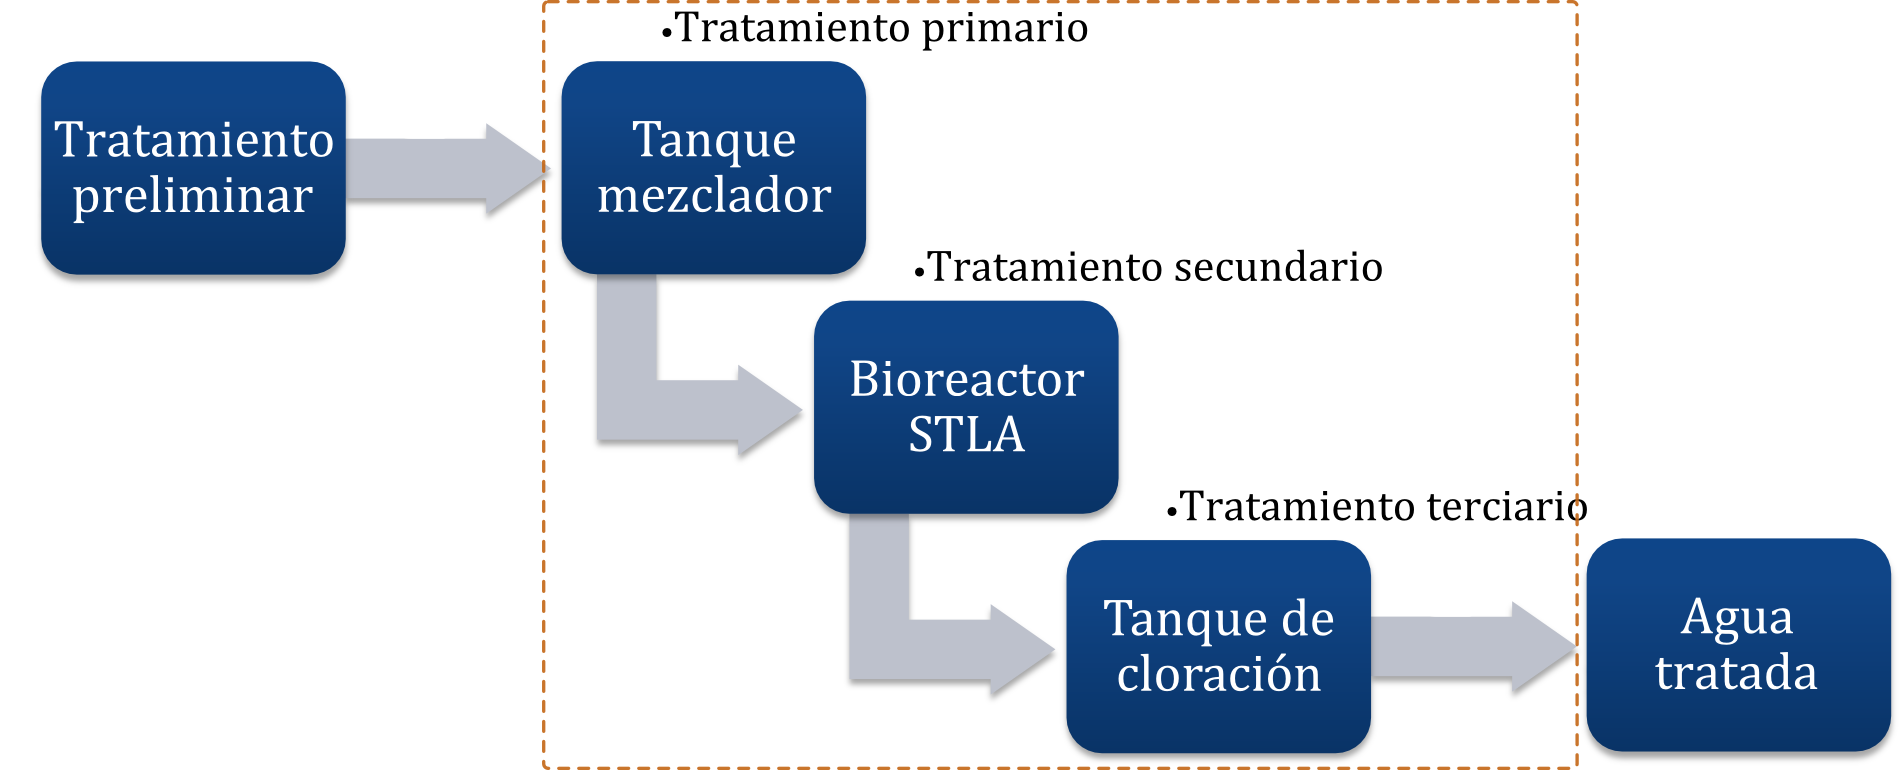
\includegraphics[scale=0.5]{Imagenes/Introduccion/PTARDiagramas.png}
	\end{center}
	\caption{Procesos de la PTAR de la UTM.} \label{fig:cap1:PTARProcess}
\end{figure}

Los par�metros importantes en el proceso de tratamiento son \cite{Cap2Bib:Tratamiento}: 
\begin{itemize} \itemsep=-0.5em
	\item \emph{pH}: La medici�n de pH es importante para el tratamiento primario y secundario. Este par�metro determina si el agua es �cida o alcalina, por lo que el valor del pH debe estar en un rango de 7 a 7.5 unidades~\cite{Cap2Bib:Metcalf}.
	\item\emph{Ox�geno Disuelto (OD)}: Para el tratamiento secundario este par�metro es fundamental, ya que determina la cantidad de ox�geno ($O_2$) disponible por los microorganismos presentes en el tratamiento secundario. Se recomienda que el valor del OD est� por arriba de $3$ a $4\frac{\milli\gram {O}_{2}}{\liter}$ \cite{Cap2Bib:Metcalf}.
	\item\emph{Temperatura}: La temperatura es importante para asegurar el crecimiento �ptimo de los microorganismos en el tratamiento secundario, se recomienda que la temperatura est� entre $28$ y $30\degreecelsius$~\cite{Cap2Bib:Metcalf}.
\end{itemize}

El monitoreo de los par�metros anteriormente mencionados, es un inicio para una futura automatizaci�n de la PTAR de la UTM, con lo cual se podr�a garantizar una minimizaci�n significativa en los costos de operaci�n, que son generados por los equipos de la planta que se mantienen en operaci�n las 24 horas del d�a, lo cual significa un gran consumo de energ�a el�ctrica \cite{Cap2Bib:Schneider}.

Por lo anterior, este proyecto de tesis plantea el dise�o y construcci�n de un sistema de monitoreo remoto para la PTAR de la UTM. El sistema que se desarroll� tiene como objetivo implementar un sistema SCADA para monitorizar de manera remota y automatizada el estado de pH, OD y temperatura de la PTAR de la UTM. El sistema almacenar� registros de mediciones y proporcionar� una GUI a trav�s de una aplicaci�n Web.

\section{Planteamiento del Problema}
\label{cap1:Planteamiento}

La necesidad inicial, que gener� este trabajo de tesis, es la automatizaci�n de la PTAR. El prop�sito de la automatizaci�n es hacer eficiente la operaci�n del sistema de aireaci�n, el cual actualmente est�n en operaci�n las 24 horas del d�a y generan un gran consumo de energ�a el�ctrica. La automatizaci�n permite que el consumo de energ�a sea sustancialmente bajo, lo cual tiene un impacto directo en los costos de operaci�n \cite{Cap2Bib:Schneider}.

Dicho lo anterior, el primer paso para la automatizaci�n de la PTAR es la caracterizaci�n de la planta. �sto se logra con un sistema de monitoreo de los par�metros que se han mencionado previamente. Por lo que, este trabajo de tesis propone el dise�o y construcci�n de un prototipo de sistema de monitoreo para la PTAR de la UTM, dicho sistema ser� implementado bajo el concepto de sistemas SCADA. 

El sistema SCADA servir� para monitorizar de manera remota y automatizada el estado de pH, OD y temperatura de la PTAR de la UTM. Dicho sistema constar� de sensores de prop�sito industrial, se almacenar� la informaci�n de las mediciones en un servidor de bases de datos y ofrecer� acceso Web mediante una GUI que permitir� visualizar el estado de los par�metros medidos de manera gr�fica y tabular.

La etapa de elementos \emph{hardware} del sistema SCADA tiene como entradas las �rdenes y peticiones provenientes de una MTU y como salidas la interacci�n con los sensores, como se ilustra en la figura~\ref{fig:cap1:PTARDiaHW}. El \emph{hardware} estar� constituido por los siguientes elementos: una etapa de acoplamiento de sensores, en la cual se realiza el acondicionamiento de se�al de los sensores, esta etapa es necesaria porque los sensores de pH, OD y temperatura requieren el uso de amplificadores operacionales de instrumentaci�n para poder operar las se�ales de dichos sensores; un sistema basado en un microcontrolador (MCU, \emph{Microcontroller Unit}) como unidad de procesamiento remota (RTU); y una interfaz de comunicaci�n serie RS-485 para establecer la comunicaci�n de la RTU con la MTU mediante el protocolo Modbus.

\begin{figure}[htb]
	\begin{center}
		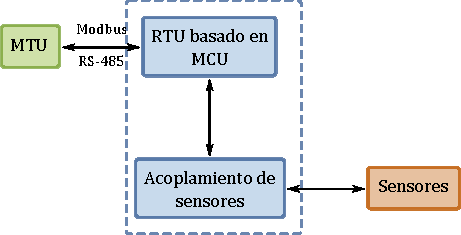
\includegraphics[scale=0.9]{Imagenes/Introduccion/PTARDiaHW.pdf}
	\end{center}
	\caption{Elementos \emph{hardware} del sistema SCADA.} \label{fig:cap1:PTARDiaHW}
\end{figure}

Los elementos \emph{software} tendr�n como entradas la interacci�n de un usuario del sistema (Administrador) y como salidas las solicitudes de monitoreo hacia la RTU, como se ilustra en la figura~\ref{fig:cap1:PTARDiaSW}. El software estar� constituido por los siguientes elementos: el \emph{software} de la MTU, que se encargar� de enviar solicitudes de monitoreo a la RTU y almacenar registros de mediciones en el servidor de base de datos; una aplicaci�n Web que se ejecutar� en un servidor, que a trav�s de una GUI permitir� la visualizaci�n de los registros de mediciones de manera gr�fica y tabular y permitir� la interacci�n del usuario final con el sistema mediante el uso de navegadores Web como \emph{Chrome}, \emph{Mozilla}, \emph{Opera}, \emph{Internet Explorer}, y otros.

\begin{figure}[htb]
	\begin{center}
		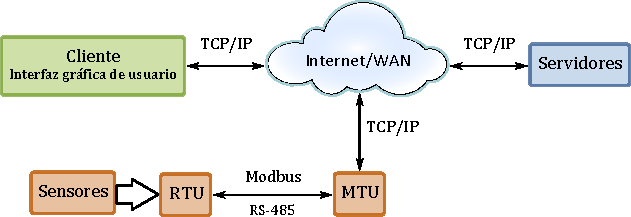
\includegraphics[scale=0.9]{Imagenes/Introduccion/PTARDiaSW.pdf}
	\end{center}
	\caption{Elementos \emph{software} del sistema SCADA.} \label{fig:cap1:PTARDiaSW}
\end{figure}

\section{Justificaci�n}
\label{cap1:Justificacion}

En la planta de tratamiento de aguas residuales de la Universidad Tecnol�gica de la Mixteca a�n no se cuenta con un sistema de monitoreo automatizado, por lo que este proceso se realiza de manera manual por los encargados.

Debido a la situaci�n anterior, es necesario dise�ar y construir un prototipo de sistema de monitoreo. Este sistema debe permitir la adquisici�n de datos de los par�metros involucrados en los procesos de tratamiento de la planta, almacenar dicha informaci�n en forma de registros en una base de datos, los cuales puedan ser visualizados por los usuarios finales a trav�s de una GUI en una aplicaci�n Web.

\section{Hip�tesis}
\label{cap1:Hipotesis}

Del prototipo de sistema de monitoreo para la planta de tratamiento de aguas residuales de la Universidad Tecnol�gica de la Mixteca, se obtendr� una herramienta para almacenar y acceder a la informaci�n del estado actual y estados previos de temperatura, pH y Ox�geno Disuelto, as� como realizar un an�lisis en base a un historial de registros de mediciones y conocer el comportamiento de la planta.

%Con el dise�o y construcci�n de un prototipo de sistema de monitoreo remoto para la PTAR de la UTM, los encargados de dicha planta podr�n tener acceso a la informaci�n acerca del estado actual y de los estados previos de temperatura, pH y Ox�geno Disuelto. Esto les permitir� realizar un an�lisis en base a un historial de registros de mediciones para conocer el comportamiento de la planta.

\section{Objetivos}
\label{cap1:Objetivos}

\subsection{Objetivo general}
\label{cap1:ObjetivoG}

Dise�ar y construir un prototipo de Sistema de Monitoreo para la Planta de Tratamiento de Aguas Residuales de la Universidad Tecnol�gica de la Mixteca.

%Dise�ar y construir un prototipo de sistema de monitoreo remoto de temperatura, pH y OD. El sistema estar� basado en un sistema SCADA con los siguientes elementos: una RTU basada en MCU, una computadora como MTU y un servidor Web y de Base de Datos. Dicho sistema almacenar�, en una base de datos, registros de mediciones tomadas de los sensores y ofrecer� una interfaz web de usuario con capacidades gr�ficas.

\subsection{Objetivos espec�ficos}
\label{cap1:ObjetivoE}

\begin{itemize} \itemsep=-0.5em
	\item Dise�ar un sistema de acondicionamiento de se�al para cada uno de los sensores haciendo uso de amplificadores operacionales de instrumentaci�n.
	\item Usar un MCU de la marca ATMEL para implementar la RTU.
	\item Hacer uso del protocolo Modbus para establecer la comunicaci�n entre la RTU y la MTU.
%	\item Implementar en el MCU el protocolo Modbus esclavo, y en la MTU el protocolo Modbus maestro.
	\item Realizar la comunicaci�n entre la RTU y la MTU a trav�s de una interfaz serie RS-485.
	\item Almacenar registros de mediciones en un servidor de base de datos MySQL.
	\item Dise�ar una aplicaci�n Web usando el \emph{framework Yii} para PHP.
\end{itemize}

\section{Contenido del documento de tesis}
\label{cap1:Contenido}

La estructura de este documento de tesis es la siguiente:

En el cap�tulo 1 se presenta una breve introducci�n acerca de los sistemas de monitoreo, el planteamiento del problema, la justificaci�n, hip�tesis y los objetivos de este proyecto de investigaci�n.

El cap�tulo 2 presenta las bases te�ricas que sustentan este proyecto de investigaci�n. Se describen las principales caracter�sticas de los sistemas SCADA, sus elementos \emph{hardware} y \emph{software}, los protocolos de comunicaci�n, se da una descripci�n de la PTAR de la UTM, los sensores con los que cuenta la UTM y las herramientas tecnol�gicas para desarrollar el sistema.

En el cap�tulo 3 se detalla el desarrollo del sistema empleando la metodolog�a de desarrollo para mejoramiento de procesos de producci�n y la metodolog�a de sistemas empotrados, por lo que se expone de manera detallada las fases de desarrollo del sistema SCADA.

El cap�tulo 4 presenta la verificaci�n y validaci�n del sistema SCADA en base a los requerimientos.

En el cap�tulo 5 se plantean las conclusiones y los futuros trabajos de investigaci�n.

Por �ltimo, se presentan las referencias bibliogr�ficas utilizadas, los diagramas esquem�ticos, el dise�o completo del circuito impreso y diagramas del dise�o software. 




		%---------------------------------------------------------------------
%
%             Cap�tulo 2
%
%---------------------------------------------------------------------

\chapter{Marco te�rico}
\label{cap2}

\section{Sistemas SCADA}
\label{cap2:SCADA}

La telemetr�a, tele-medida o medida a distancia, es requerida para conectar equipos y sistemas separados por distancias muy grandes, principalmente en procesos industriales, procesos de manufactura moderna, industria minera, industrias de seguridad y otras. El rango de distancia puede ser desde unos cuantos metros a miles de kil�metros. La telemetr�a es usada para enviar �rdenes, programas y recibir informaci�n de monitoreo desde ubicaciones remotas (Monitoreo Remoto) \cite{Cap2Bib:PracticalScada, Cap2Bib:SistemasScada}.\par

Un sistema de monitoreo remoto (\emph{Remote Monitoring System}) se define como un sistema que permite realizar rutinariamente monitoreo y supervisi�n a trav�s de una infraestructura de red \cite{Cap2Bib:Esarda, Cap2Bib:TesisDavid}.\par 

El concepto de Control con Supervisi�n y Adquisici�n de Datos (SCADA, \emph{Supervisory Control and Data Acquisition}) se refiere a la combinaci�n de telemetr�a y adquisici�n de datos. Se da el nombre de SCADA a cualquier sistema que consta de componentes \emph{hardware} y \emph{software}, el cual permite el acceso a datos remotos y el control de un proceso mediante el uso de sistemas de comunicaciones.\par

Actualmente, los sistemas SCADA son usados por las empresas industriales modernas en aplicaciones como: plantas de energ�a, telecomunicaciones, transporte, tratamiento de agua y desechos, etc., en donde los componentes \emph{hardware} obtienen los datos y los emiten a una computadora, la cual cuenta con \emph{software} para procesamiento de la informaci�n y para mostrarla en pantallas personalizadas (interfaces gr�ficas). De esta manera, los sistemas SCADA permiten a los operadores monitorizar y controlar los equipos desde una estaci�n central.\par

Los sistemas SCADA han evolucionado en paralelo con las tecnolog�as modernas, y con ello la mayor�a de dichos sistemas presentan dos topolog�as:\par

\begin{itemize} \itemsep=-0.5em

\item \emph{Sistemas SCADA centralizados}: En los sistemas centralizados o monol�ticos, una computadora central es la encargada de realizar el monitoreo completo de la planta (industrial) y todos la informaci�n es almacenada en una base de datos dentro de la misma computadora \cite{Cap2Bib:PracticalScada}. Este tipo de red SCADA se implementa para comunicarse con unidades terminales remotas (RTU, \emph{Remote Terminal Unit}) en el �rea de campo y a trav�s de buses de campo (FieldBus) \cite{Cap2Bib:IndustrialCT}, tal como se ilustra en la figura~\ref{fig:cap2:SCADA:mon}.

Las desventajas comunes de los sistemas SCADA centralizados o monol�ticos son: para un sistema peque�o los costos iniciales son bastante altos y debido al tama�o fijo del sistema, una expansi�n gradual para la mejora de la planta no es posible.

\item \emph{Sistemas SCADA distribuidos}: Un sistema SCADA distribuido es soportado por un conjunto de computadoras, las cuales est�n interconectadas a trav�s de una red y cuyos componentes de \emph{software} se encuentran dispersos entre dichas computadoras para realizar las tareas de manera colaborativa, lo cual permite la escalabilidad del sistema \cite{Cap2Bib:PracticalScada, Cap2Bib:PAInternet, Cap2Bib:ApDistribuidas}. Un sistema SCADA distribuido generalmente hace uso de la arquitectura cliente/servidor.
\end{itemize}

\begin{figure}[htb]
	\begin{center}
		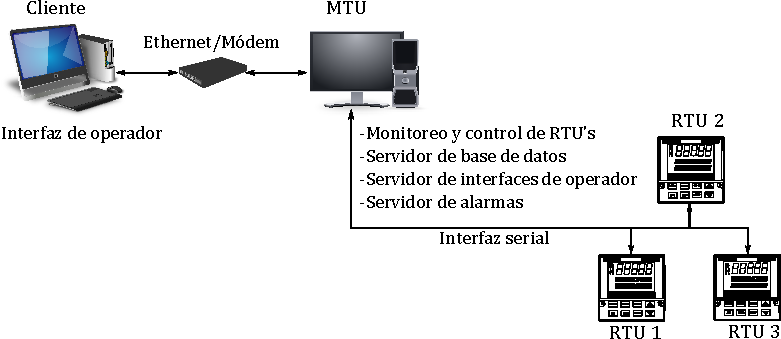
\includegraphics[scale=0.9]{Imagenes/MarcoTeorico/SCADAMonolitico.pdf}
	\end{center}
	\caption{Configuraci�n de un sistema SCADA centralizado.} \label{fig:cap2:SCADA:mon}
\end{figure}

Debido a las desventajas que presentan los sistemas SCADA centralizados, en este proyecto de investigaci�n se implementar� un sistema SCADA distribuido, por lo que en esta secci�n se har� �nfasis a la teor�a relacionada con sistemas SCADA distribuidos.

Ahora, cada computadora dentro de un sistema SCADA distribuido tiene una funci�n espec�fica, por ejemplo: algunas computadoras sirven como procesadores de comunicaci�n con dispositivos de campo o RTUs; otras sirven como interfaces de operador que proporcionan interfaces humano m�quina (HMI, \emph{Human Machine Interface}); y algunas computadoras se utilizan como servidores de bases de datos para procesamiento de informaci�n \cite{Cap2Bib:IndustrialCT}. En la figura~\ref{fig:cap2:SCADA:dist} se ilustra una configuraci�n t�pica de un sistema SCADA distribuido.\par

La distribuci�n de funciones provee una mayor capacidad de procesamiento comparado con un sistema que consta de una sola computadora. Las tareas esenciales de un sistema SCADA distribuido, que requieren procesamiento de manera individual, son las siguientes \cite{Cap2Bib:PracticalScada, Cap2Bib:IndustrialCT}:

\begin{itemize} \itemsep=-0.5em
	\item \emph{Entradas y salidas}: Son la interfaz entre el sistema de monitoreo y las instalaciones de la planta.
	\item \emph{Bases de datos}: Se encarga de almacenar todos los datos provenientes de las entradas y salidas, al mismo tiempo permite el acceso a esta informaci�n, de tal manera que las dem�s tareas puedan realizar sus funciones.
	\item \emph{Alarmas}: Esta tarea administra todas las alarmas del sistema a trav�s de la comparaci�n de las entradas con un valor de umbral predeterminado.
	\item \emph{Tendencias}: Captura todos los datos de las variables que se desean monitorizar con el prop�sito de mostrar su evoluci�n con respecto al tiempo.
	\item \emph{Reportes}: Los reportes son generados a partir de los datos de la planta y pueden ser creados a petici�n del usuario u operador.
	\item \emph{Presentaci�n}: Administra todos los datos que el operador va a monitorizar a trav�s de una GUI \cite{Cap2Bib:Automatizacion}.
\end{itemize}

\begin{figure}[htb]
	\begin{center}
		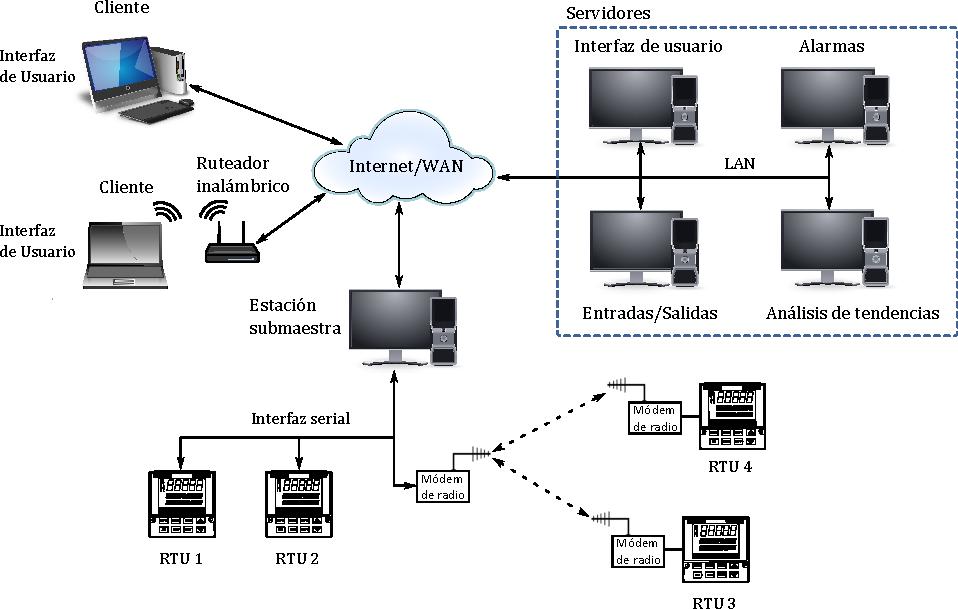
\includegraphics[scale=0.9]{Imagenes/MarcoTeorico/SCADADistribuido.pdf}
	\end{center}
	\caption{Configuraci�n de un sistema SCADA distribuido.} \label{fig:cap2:SCADA:dist}
\end{figure}

\subsection{Componentes \emph{hardware} de un sistema SCADA distribuido}
\label{cap1:SCADA:HW}
En esta secci�n se aborda el concepto de sistemas de telemetr�a (sistemas de medici�n a distancia) y sus fundamentos con base a la arquitectura de un sistema SCADA distribuido. Por lo tanto, se describen los componentes \emph{hardware} (figura~\ref{fig:cap2:SCADA:dist:HW}), los cuales se han clasificado en los siguientes niveles de jerarqu�a \cite{Cap2Bib:PracticalScada, Cap2Bib:SistemasScada, Cap2Bib:IndustrialCT}:

\begin{figure}[htb]
	\begin{center}
		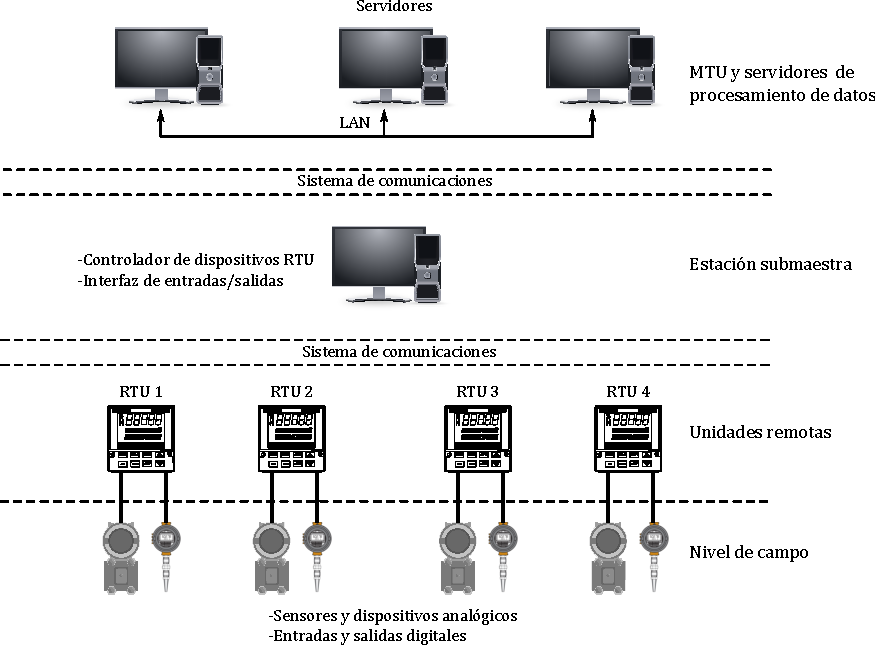
\includegraphics[scale=0.9]{Imagenes/MarcoTeorico/SCADAHW.pdf}
	\end{center}
	\caption{Niveles de jerarqu�a de \emph{hardware} en un sistema SCADA.} \label{fig:cap2:SCADA:dist:HW}
\end{figure}

\begin{itemize} \itemsep=-0.5em
	\item Dispositivos de instrumentaci�n y control a nivel de campo\footnote{Los dispositivos de campo son los que est�n en contacto directo con la planta industrial.}.
	\item Uno o m�s dispositivos de interfaces de datos de campo. Dichos dispositivos son las RTUs que desempe�an el papel de interfaz con los dispositivos de instrumentaci�n y control a nivel campo.
	\item Un servidor o conjunto de servidores como sistema central, los cuales usualmente son denominados como centro del sistema SCADA, estaciones maestras o MTUs. La MTU de un sistema distribuido consta de un conjunto de servidores que realizan las tareas de: entradas y salidas, bases de datos, alarmas, tendencias, reportes y presentaci�n.
	\item Un sistema de comunicaciones para el intercambio de datos entre RTUs y MTUs.
	%Este sistema puede ser radio, l�nea telef�nica, cableado, microondas, fibra �ptica, sat�lite, o bien puede ser cualquier combinaci�n de �stos.
\end{itemize}

\subsubsection{Instrumentaci�n}

La instrumentaci�n electr�nica se aplica en el sensado y procesamiento de la informaci�n proveniente de variables f�sicas\footnote{Temperatura, presi�n, volumen, etc.} y de otro tipo\footnote{Variables de referencia en dispositivos de control o variables de umbral en sistemas de alarmas.}, a partir de las cuales se realiza el monitoreo y control de procesos, empleando dispositivos y tecnolog�as electr�nicas.

Para su funcionamiento la instrumentaci�n se divide en tres etapas: 

\begin{itemize} \itemsep=-0.5em
	\item \emph{Los sensores}: Son aquellos que transforman la magnitud de una variable f�sica que se desea medir a una se�al el�ctrica.
	\item \emph{Acondicionamiento}: Como su nombre lo indica, acondiciona los niveles de la se�al de salida de un sensor. Esto se debe a que en la mayor�a de los casos la se�al de los sensores suele no ser adecuada para su procesamiento. En general los sensores entregan se�ales muy peque�as y vulnerables a ruido, por lo que el acondicionamiento generalmente consiste de dos subetapas: la etapa de amplificaci�n y la etapa de filtrado. Dichas subetapas se realizan a trav�s de un amplificador operacional de instrumentaci�n.
	\item \emph{Digitalizaci�n}: La digitalizaci�n proporciona un c�digo digital (binario) equivalente a la se�al de entrada proveniente de la etapa de acoplamiento. Dicho c�digo permite el procesamiento de las se�ales a trav�s de sistemas basados en MCU, procesadores o computadoras.
\end{itemize}

\subsubsection{Componentes de la RTU}

Una RTU es una unidad independiente cuyas tareas son: adquisici�n de datos, gesti�n de equipos de control en un proceso industrial (ubicado en un lugar remoto) y transferir dichos datos a la MTU \cite{Cap2Bib:PracticalScada}.

Generalmente una RTU consiste en un sistema empotrado (\emph{Embedded System}), el cual tiene como unidad principal un procesador \cite{Cap2Bib:TesisDavid}. La complejidad de la unidad central de procesamiento determina la clasificaci�n del sistema empotrado, microprocesador ($\micro$P) o MCU.

La ventaja de un dise�o basado en MCU sobre uno basado en $\micro$P radica en que el MCU incluye internamente tres unidades funcionales: unidad central de procesamiento (CPU, \emph{Central Processing Unit}), memoria de c�digo/datos y perif�ricos de entrada y salida. En cambio, un $\micro$P necesita de las mismas unidades funcionales pero de manera externa. Un dise�o basado en MCU reduce significativamente el tiempo de desarrollo, el tama�o del dispositivo y el costo \cite{Cap2Bib:TesisDavid}. La figura~\ref{fig:cap2:SCADA:dist:HW:RTU} muestra la configuraci�n t�pica de una RTU basada en MCU.

\begin{figure}[htb]
	\begin{center}
		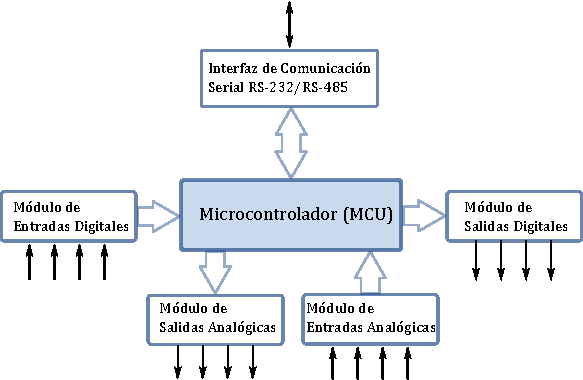
\includegraphics[scale=0.9]{Imagenes/MarcoTeorico/SCADA-RTU.pdf}
	\end{center}
	\caption{Configuraci�n de una RTU basada en MCU.} \label{fig:cap2:SCADA:dist:HW:RTU}
\end{figure}

La configuraci�n de una RTU basada en MCU est� formada por los siguientes m�dulos \emph{hardware} \cite{Cap2Bib:PracticalScada, Cap2Bib:SistemasScada}:

\begin{itemize} \itemsep=-0.5em
\item \emph{Unidad central de procesamiento}: La CPU es la encargada de procesar las instrucciones almacenadas en la memoria de c�digo. Por lo tanto, la CPU tiene acceso a las memorias (de datos y de c�digo), realiza los c�lculos asociados o requeridos, controla perif�ricos de entrada y salida, y perif�ricos de interfaz de comunicaci�n.

Las instrucciones almacenadas en la memoria de c�digo forman la configuraci�n y el programa de control propias de la RTU. La configuraci�n y el programa de control establecen los par�metros para: perif�ricos de entrada y salida (anal�gicas y digitales); la comunicaci�n entre la RTU y la MTU, la cual generalmente consiste en un protocolo industrial de control y monitoreo \cite{Cap2Bib:TesisDavid}; y, los programas de aplicaci�n de la RTU, tal es el caso de un control anal�gico de lazo cerrado PID (\emph{Proporcional Integral Diferencial}).

\item \emph{Entradas anal�gicas}: Estos perif�ricos permiten la adquisici�n de datos de las se�ales que proporcionan los m�dulos de instrumentaci�n (sensores y acondicionamiento).

El elemento principal de este m�dulo es un convertidor an�logo-digital (ADC, \emph{Analog-Digital Converter}), cuya funci�n es tomar un voltaje anal�gico como entrada y entregar como salida un c�digo digital (c�digo binario) correspondiente a dicho voltaje de entrada (figura~\ref{fig:cap2:SCADA:dist:HW::RTU:ADC}). Este c�digo digital es adecuado para su procesamiento a trav�s de un MCU.

\item \emph{Salidas anal�gicas}: Un perif�rico de salida anal�gica en general consiste de dos m�dulos: un registro de salidas digitales (usualmente 8 bits) y un convertidor digital-an�logo (DAC, \emph{Digital-Analog Converter}). El DAC es un dispositivo que recibe un c�digo digital (binario) y genera un nivel de voltaje de salida (anal�gico), como se ilustra en la figura~\ref{fig:cap2:SCADA:dist:HW::RTU:DAC}.

En una RTU, una salida anal�gica frecuentemente se usa como voltaje de referencia para el controlador de alg�n dispositivo anal�gico, como puede ser el controlador de un motor, una bomba, un sistema de enfriamiento, un calefactor, etc. Una salida anal�gica tambi�n puede ser usada como fuente de alimentaci�n para dispositivos de bajo consumo de energ�a, por ejemplo, la alimentaci�n o polarizaci�n de un sensor de Ox�geno Disuelto y otros.

\item \emph{Entradas y salidas digitales}: Las entradas y salidas digitales se usan para indicar informaci�n como se�ales de estados l�gicos de alarmas y otros dispositivos. Por ejemplo el estado (encendido o apagado) de un relevador que controla una v�lvula, un actuador o cualquier dispositivo anal�gico o de las alarmas que indican el estado cr�tico de alguna variable en el proceso de una RTU. Dichas alarmas son procesadas por la MTU para tomar medidas de control o simplemente mostrarlas en una pantalla de operador.

Es importante considerar un aislamiento adecuado para las entradas y salidas digitales, ya que los perif�ricos de un MCU normalmente operan con niveles de voltaje TTL. Una buena opci�n es emplear dispositivos de aislamiento �ptico, relevadores o transformadores.

\item \emph{Interfaces de comunicaci�n}: En una RTU, para la comunicaci�n con la MTU, se pueden manejar diferentes interfaces de comunicaci�n seg�n sean las necesidades. Actualmente, las interfaces de comunicaci�n que una RTU debe soportar abarcan: interfaces serie RS-232/RS-485, l�nea telef�nica, fibra �ptica, microondas, sat�lite o radio v�a portadora (VHF, UHF o 900 MHz).
\end{itemize}

\begin{figure}[htb]
	\begin{center}
		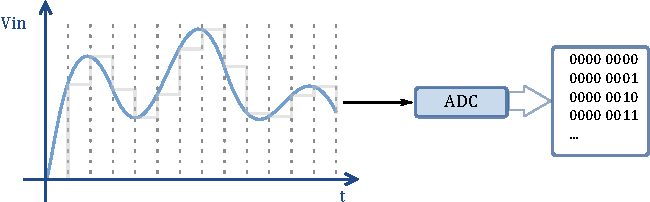
\includegraphics[scale=0.9]{Imagenes/MarcoTeorico/SCADA-RTU-ADC.pdf}
	\end{center}
	\caption{Funci�n del ADC.} \label{fig:cap2:SCADA:dist:HW::RTU:ADC}
\end{figure}

\begin{figure}[htb]
	\begin{center}
		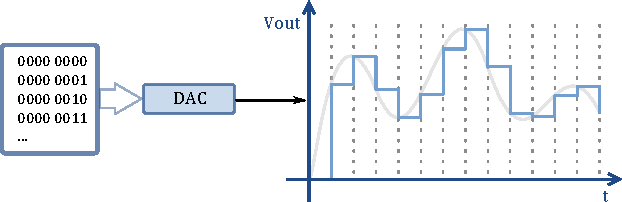
\includegraphics[scale=0.9]{Imagenes/MarcoTeorico/SCADA-RTU-DAC.pdf}
	\end{center}
	\caption{Funci�n del DAC.} \label{fig:cap2:SCADA:dist:HW::RTU:DAC}
\end{figure}

\subsubsection{Componentes de la MTU}

Una MTU es el centro de un sistema SCADA y est� formada por un servidor o conjunto de servidores (usualmente computadoras) interconectados a trav�s de una red para realizar tareas de manera colaborativa. La MTU es la que inicia toda la comunicaci�n con las RTUs, re�ne los datos, almacena la informaci�n, realiza el procesamiento y proporciona las interfaces de usuario para los operadores \cite{Cap2Bib:PracticalScada, Cap2Bib:SistemasScada, Cap2Bib:IndustrialCT}.
 
Las funciones principales de una MTU son obtener peri�dicamente los datos de campo de las RTUs, monitorizar y controlar remotamente los dispositivos a trav�s de las estaciones de operador. Los componentes y caracter�sticas b�sicas de una MTU son:

\begin{itemize} \itemsep=-0.5em
\item \emph{Servidores e interfaz de operador}: Una MTU consta de una o m�s estaciones (computadoras) de operador, las cuales cuentan con una interfaz de usuario para mostrar el estado de las RTUs y permitir el control al operador; un servidor para el manejo de bases de datos; el servidor de alarmas; un servidor de presentaci�n, el cual muestra la evoluci�n de las variables monitoreadas a trav�s de gr�ficas de tendencias; un servidor para generar reportes; un servidor de interfaces de usuario; y un servidor de entradas y salidas, el cual tiene bajo su control a los dispositivos de campo (RTU), este servidor tambi�n es conocido como el controlador de las RTUs. 

\item \emph{Software de la MTU}: El \emph{software} en una MTU se divide en dos categor�as: el sistema operativo, el cual puede ir desde un sistema MS-DOS, Windows, Windows NT a los distintos sistemas Unix (Linux) y el \emph{software} del sistema SCADA, generalmente consiste en la adquisici�n de datos, control, archivado o almacenamiento en base de datos y la interfaz de operador o HMI.

\item \emph{Interfaces de comunicaci�n}: La MTU establece la comunicaci�n con las RTUs a trav�s de una interfaz de comunicaci�n. %como las que se mencionaron en la secci�n~\ref{cap2:SCADA:dist:HW}. 
Esta comunicaci�n generalmente se realiza haciendo uso de buses de campo\footnote{El t�rmino ``bus de campo'' engloba varios protocolos de control industrial, por ejemplo Modbus, PROFIBUS, WorldFIP y CAN}.
\end{itemize}

Las estaciones de operador y los servidores de la MTU se intercomunican haciendo uso de las tecnolog�as de redes LAN, WAN, Internet y la suite de protocolos TCP/IP.

Para distribuir el procesamiento a trav�s de los m�ltiples servidores, los sistemas SCADA distribuidos hacen uso de las siguientes tecnolog�as\cite{Cap2Bib:Cisco}: redes de �rea local (LAN, \emph{Local Area Network}), tal es el caso de la familia de redes Ethernet o est�ndar IEEE 802.3; las redes de �rea amplia (WAN, \emph{Wide Area Network}); y la suite de protocolos de Internet, de los cuales los m�s conocidos globalmente son el Protocolo de Control de Transmisi�n (TCP, \emph{Transmission Control Protocol}) y el Protocolo de Internet (IP, \emph{Internet Protocol}), estos protocolos forman parte de un conjunto de protocolos conocidos como TCP/IP.

%En casos particulares de sistemas SCADA es necesario instalar estaciones submaestras, las cuales permiten obtener sitios de control dentro de una regi�n espec�fica. Una estaci�n submaestra tiene las siguientes funcionalidades:

%\begin{itemize}\itemsep=-0.5em
%\item Adquisici�n de datos de las RTUs dentro de la regi�n asignada.
%\item Registrar y mostrar estos datos en una estaci�n local de operador.
%\item Pasar los datos a la MTU.
%\item Proporcionar a las RTUs, dentro de su regi�n, las peticiones de control provenientes de la MTU.
%\end{itemize}

\subsection{Componentes \emph{software} del sistema SCADA distribuido}

El \emph{software} de un sistema SCADA distribuido es multitareas y est� basado principalmente en bases de datos de tiempo real localizados en uno o m�s servidores. La arquitectura general del \emph{software} de un sistema SCADA se ilustra en la figura~\ref{fig:cap2:SCADA:dist:SW} y sus componentes son \cite{Cap2Bib:PracticalScada, Cap2Bib:SistemasScada, Cap2Bib:IndustrialCT}:

\begin{figure}[htb]
	\begin{center}
		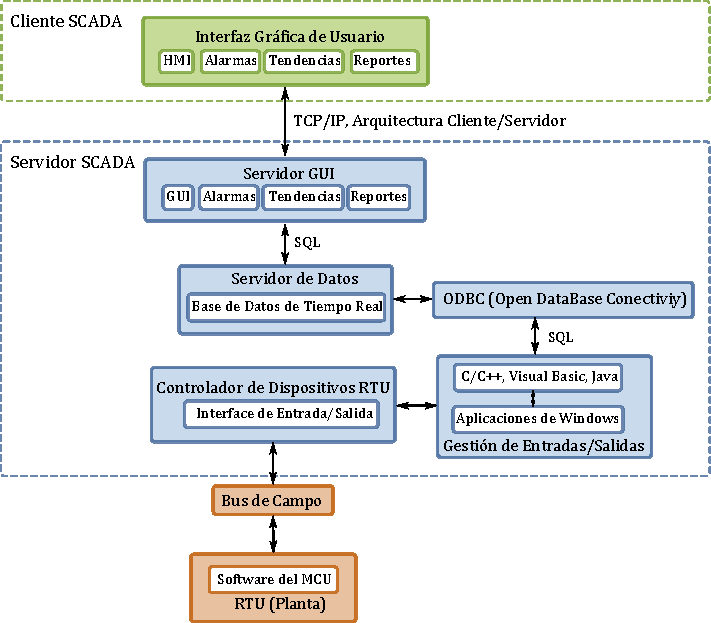
\includegraphics[scale=0.9]{Imagenes/MarcoTeorico/SCADASW.pdf}
	\end{center}
	\caption{Arquitectura general del \emph{software} de un sistema SCADA.} \label{fig:cap2:SCADA:dist:SW}
\end{figure}

\begin{itemize}\itemsep=-0.5em
\item Interfaz de usuario.
\item Servidor de representaciones gr�ficas de tendencias.
\item Servidor de alarmas y eventos.
\item Servidor para generaci�n de reportes.
\item Bases de datos.
\item Acceso a los datos.
\item Manejo de redes.
\item Interfaces RTU.
\end{itemize}

Generalmente, los componentes de interfaz de usuario, representaciones gr�ficas, servidor de alarmas y eventos, servidor de reportes y servidor de bases de datos, consisten en aplicaciones distribuidas con arquitectura cliente/servidor, de las cuales las aplicaciones Web son las m�s conocidas globalmente. En cambio las aplicaciones para interfaces RTU se desarrollan empleando lenguajes de programaci�n como C/C++, Visual Basic y Java.

\subsubsection{Comunicaci�n con dispositivos de campo}

Los servidores de datos realizan solicitudes peri�dicamente a los controladores de dispositivos de campo (RTU). La comunicaci�n entre la MTU y la RTU globalmente se realiza a trav�s de buses de campo, por ejemplo Modbus, PROFIBUS, WorldFIP y CAN. Por lo tanto el \emph{software} SCADA debe proporcionar las herramientas necesarias para llevar a cabo dicha comunicaci�n \cite{Cap2Bib:PracticalScada, Cap2Bib:IndustrialCT}.

\subsubsection{Comunicaci�n entre aplicaciones}

La comunicaci�n interna entre el conjunto de servidores para procesamiento de datos, se realiza usando la arquitectura distribuida cliente/servidor. En general esta comunicaci�n se realiza mediante la suite de protocolos TCP/IP \cite{Cap2Bib:PracticalScada, Cap2Bib:IndustrialCT}.

Los m�todos m�s conocidos para el intercambio de informaci�n entre las aplicaciones de los servidores son ODBC (\emph{Open Data Base Conectivity}) y SQL (\emph{Structured Query Language}) \cite{Cap2Bib:SistemasScada}.

\paragraph{ODBC}
ODBC es una tecnolog�a de Microsoft Windows y es un est�ndar que permite a las aplicaciones el acceso a datos en sistemas de gesti�n de bases de datos (DBMS, \emph{Data Base Managment Systems}) utilizando SQL como m�todo est�ndar de acceso \cite{Cap2Bib:SistemasScada}.

Una aplicaci�n desarrollada en lenguajes est�ndares de programaci�n (C, C++, Visual Basic o Java), necesita la inclusi�n del controlador ODBC correspondiente para tener acceso a distintas bases de datos, dicho controlador es una librer�a de enlace din�mico (DLL, \emph{Dynamic Link Library}).

La interfaz ODBC define los siguientes aspectos: una librer�a de llamadas a funciones ODBC, la sintaxis SQL necesaria, c�digos de error est�ndar, el m�todo de conexi�n a un DBMS y el formato de presentaci�n de los datos.

\paragraph{SQL}
SQL es un est�ndar para la comunicaci�n con bases de datos, que permite una interfaz com�n para el acceso a los datos por parte de cualquier aplicaci�n que se apegue a dicho est�ndar \cite{Cap2Bib:SistemasScada}.

Las posibilidades de esta tecnolog�a incluyen: 

\begin{itemize}\itemsep=-0.5em
\item \emph{Procedimientos}: Son bibliotecas de �rdenes almacenadas en la base de datos que permiten reducir el tr�fico en la red y simplifican los procedimientos de acceso a los usuarios de las bases de datos.
\item \emph{Eventos}: Son �rdenes que se activan de forma autom�tica bajo unas ciertas condiciones, facilitando el mantenimiento de la integridad de los datos.
\item \emph{Replicaci�n}: Permite la duplicaci�n y sincronizaci�n de bases de datos; la accesibilidad, permite el intercambio o env�o de informaci�n bas�ndose en eventos.
\end{itemize}

\subsubsection{Bases de datos relacionales}

Las bases de datos relacionales (\emph{Relational Data Base}) proporcionan estructuras de datos, independientemente del tipo de aplicaciones que acceden a �stos o de su estructura \cite{Cap2Bib:SistemasScada}.

Una base de datos relacional es un conjunto de tablas de datos que contienen campos. �stos sirven como nexos de uni�n a trav�s de los cuales se pueden establecer m�ltiples combinaciones. Las combinaciones posibles pr�cticamente son ilimitadas, todo depende de la configuraci�n del m�todo de b�squeda (consulta, \emph{Query}), o el tipo de datos que se requiera consultar.

Este tipo de organizaci�n permite el uso de la arquitectura cliente/servidor y con ello se simplifican la administraci�n de los datos y las aplicaciones que los usan, se disminuye el espacio de almacenamiento y se reducen los problemas asociados a las bases de datos redundantes. 

Los usuarios y las aplicaciones pueden acceder a los datos de forma r�pida y sencilla, ya que pueden personalizar sus propias consultas y obtener los datos de acuerdo a sus necesidades.

\subsubsection{Interfaces de usuario (UI)}

El t�rmino ``interfaz gr�fica de usuario'' (GUI) se refiere a los m�todos y dispositivos usados en la interacci�n entre m�quinas y los seres humanos que las usan. La interfaz de usuario de un sistema mec�nico, un veh�culo o las instalaciones de una industria, frecuentemente es llamada HMI \cite{Cap2Bib:SistemasScada}.

En un sistema de control industrial, una HMI se usa para proporcionar a los operadores informaci�n de una m�quina o planta y permite monitorizar, controlar y archivar dicho sistema. Por lo tanto, las tareas fundamentales que una HMI debe realizar son: la comunicaci�n de informaci�n de la m�quina al usuario y la comunicaci�n de informaci�n del usuario a la m�quina.

Las HMI de tipo supervisoras son usadas en sistemas en donde la distancia, entre la estaci�n de control y la estaci�n remota (o planta), es considerablemente grande. Las HMI de este tipo son propias de un sistema SCADA, en el cual se encuentran dispositivos tales como bombas, ventiladores o indicadores de purificaci�n de aguas.

Una HMI de un sistema SCADA permite que desde una interfaz de operador se pueda monitorizar completamente la planta y muestra una representaci�n gr�fica del estado actual de cada componente, el estado de las alarmas que indican cuando alg�n par�metro est� fuera del rango de operaci�n adecuado. Estas tareas se realizan gracias a la retroalimentaci�n por parte de los sensores que miden los par�metros de los procesos en la planta.

\subsection{SCADA en la Internet}

La Internet es simplemente la red virtual en donde todas las estaciones se interconectan f�cilmente sin tener que preocuparse por las conexiones f�sicas.

Actualmente el modelo de Internet gira en torno a la suite de protocolos abiertos TCP/IP \cite{Cap2Bib:PracticalScada, Cap2Bib:RedesComp}, en donde el protocolo IP ofrece la capacidad de realizar el ruteo permitiendo que los paquetes sean enviados a trav�s de redes interconectadas con topolog�as diferentes y el protocolo TCP permite que los paquetes sean enviados desde un punto a otro garantizando que lleguen a su destino.

El protocolo de aplicaci�n m�s usado en Internet es el protocolo de transferencia de hipertexto (HTTP, \emph{Hypertext Transfer Protocol}), el cual es la base para la WWW (\emph{World Wide Web}). El protocolo HTTP es de arquitectura cliente/servidor, por lo tanto, el uso m�s frecuente que se le da es el de un navegador (cliente) que accede a un servidor Web. Los datos que pueden ser transferidos por este protocolo son: texto nativo, hipertexto, audio, im�genes, etc.

El protocolo HTTP permite el desarrollo de aplicaciones de interfaces gr�ficas de usuario para sistemas SCADA, ya que es posible transferir representaciones gr�ficas y estados de los dispositivos de campo. Adem�s, la arquitectura cliente/servidor permite que m�s de un usuario u operador acceder al sistema SCADA a trav�s de un navegador Web ejecutado en una computadora desde cualquier lugar permitiendo el monitoreo y control de la planta como si el operador estuviese en las instalaciones de la misma.

\section{Planta de tratamiento de aguas residuales de la UTM}

\subsection{El Agua Residual}

Esencialmente el agua residual, es el agua usada por una comunidad en una gran variedad de aplicaciones. Seg�n la Norma Oficial Mexicana \emph{NOM-001-ECOL-1996} emitida por la Secretar�a de Medio Ambiente y Recursos Naturales (SEMARNAT) \cite{Cap2Bib:NOM001}, se definen las aguas residuales como: 

\emph{``Las aguas de composici�n variada provenientes de las descargas de usos municipales, industriales, comerciales, de servicios, agr�colas, pecuarios, dom�sticos, incluyendo fraccionamientos y en general cualquier otro uso, as� como la mezcla de ellas''.}

Las fuentes principales de aguas residuales son \cite{Cap2Bib:TesisIzcoatl, Cap2Bib:Metcalf1}: 
\begin{itemize}\itemsep=-0.5em
\item \emph{Las aguas residuales dom�sticas}: Engloban las aguas residuales generadas por los hogares, instalaciones comerciales e instituciones p�blicas. La contaminaci�n es org�nica en su mayor�a, compuesta de materia fecal, papel, jab�n, suciedad, restos de alimentos (basura) y otras sustancias.
\item \emph{Las aguas residuales industriales}: En donde predominan los desechos industriales, est�n en funci�n del tipo y tama�o de la industria. Algunas son aguas de enjuague; otras se encuentran muy cargadas de materia org�nica o mineral, o con sustancias corrosivas, venenosas, inflamables o explosivas.
\end{itemize}

\subsection{Sistema de tratamiento de aguas residuales de la UTM}

Los m�todos de tratamiento de aguas residuales en donde predomina la aplicaci�n de fuerzas de contacto f�sico son conocidos como unidades de operaci�n. Los m�todos de tratamiento de aguas residuales en los cuales la eliminaci�n de contaminantes se realiza a trav�s de reacciones qu�micas o biol�gicas son conocidos como unidades de procesamiento. Ambos m�todos son agrupados para permitir varios niveles de tratamiento conocidos como: preliminar, primario, secundario y avanzado (o terciario) \cite{Cap2Bib:Metcalf7}.

Los niveles de tratamiento (Figura~\ref{fig:cap2:PTAR}) con los que cuenta la PTAR de la UTM son los siguientes \cite{Cap2Bib:TesisIzcoatl}:
\begin{itemize}\itemsep=-0.5em

\item \emph{Tratamiento preliminar}: Consiste en un sistema de rejas o cribas (figura~\ref{fig:cap2:PTAR:rej}) para separar los s�lidos mayores o flotantes y con ello proteger los equipos de los siguientes niveles de tratamiento. 

\item \emph{Tratamiento primario}: Emplea el proceso f�sico de asentamiento en un tanque de sedimentaci�n, para eliminar la mayor�a de los s�lidos suspendidos y sedimentales que se encuentran en el agua residual. Este proceso utiliza un tanque mezclador (figura~\ref{fig:cap2:PTAR:Mez}) para homogenizar el efluente (agua residual) y controlar el flujo de entrada al siguiente tratamiento.

\item \emph{Tratamiento secundario}: Emplea el proceso biol�gico conocido como Sistema de Tratamiento por Lodos Activados (STLA), para remover la mayor parte de la materia org�nica del agua residual. La biodegradaci�n de la materia org�nica se lleva a cabo en un bioreactor (figura~\ref{fig:cap2:PTAR:STLA}).

\item \emph{Tratamiento terciario}: En donde se utiliza un tanque (figura~\ref{fig:cap2:PTAR:Cl}) para adherir una soluci�n de hipoclorito de sodio (o cloro) para la eliminaci�n de bacterias.

\end{itemize}

\begin{figure}[htb]
	\begin{center}
		\begin{tabular}{cc}
			\subfloat[Tratamiento preliminar.]{%
				\label{fig:cap2:PTAR:rej}%
				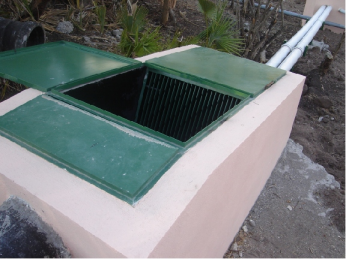
\includegraphics[scale=0.78]{Imagenes/MarcoTeorico/Rejillas.png}} &
			\subfloat[Tratamiento primario.]{%
				\label{fig:cap2:PTAR:Mez}%
				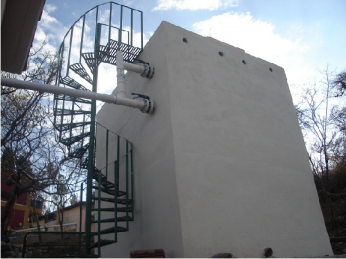
\includegraphics[scale=0.78]{Imagenes/MarcoTeorico/Mezclador.png}} \\
			\subfloat[Tratamiento secundario.]{%
				\label{fig:cap2:PTAR:STLA}%
				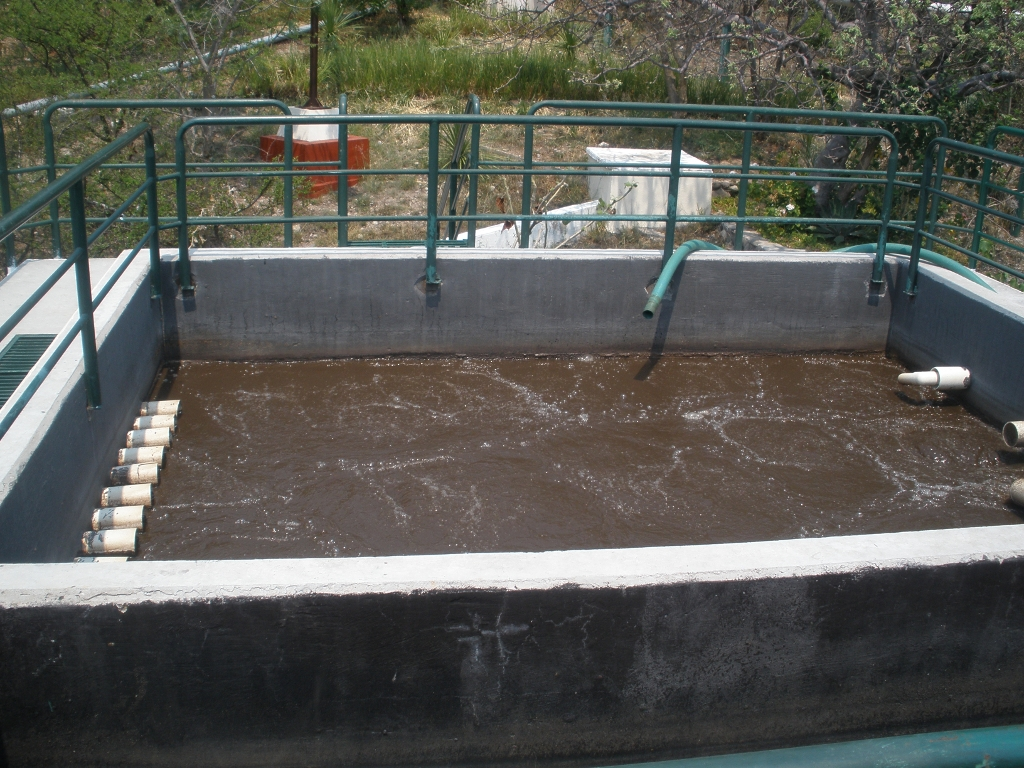
\includegraphics[scale=0.2]{Imagenes/MarcoTeorico/Bioreactor.JPG}} &
			\subfloat[Tratamiento terciario.]{%
				\label{fig:cap2:PTAR:Cl}
				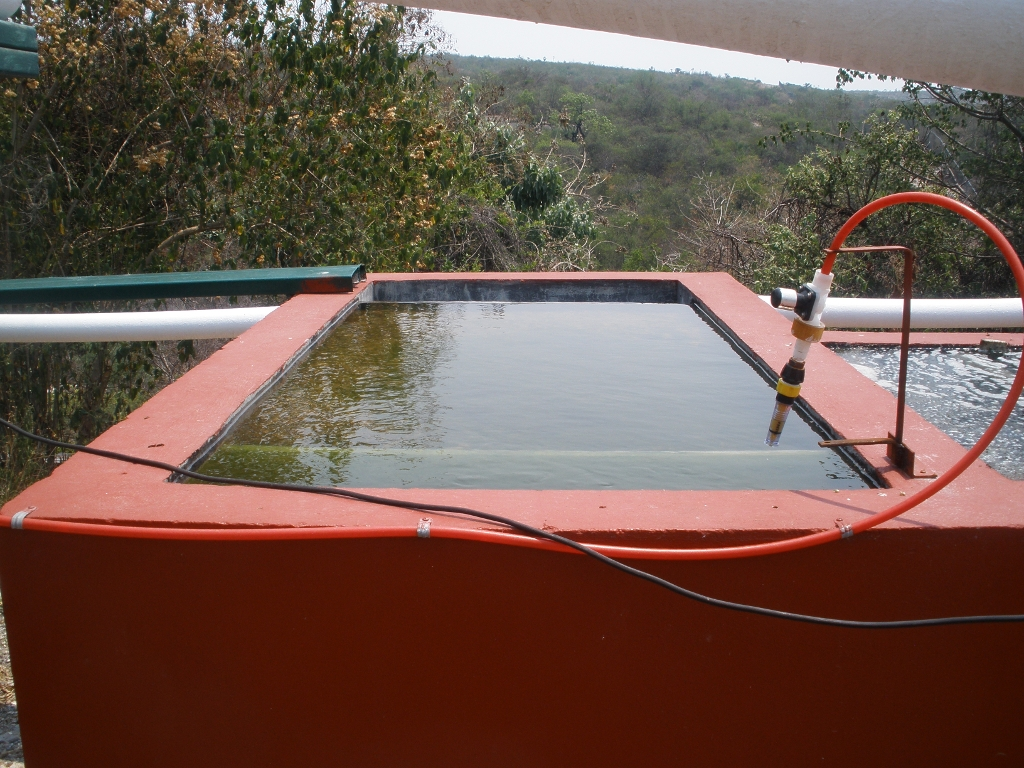
\includegraphics[scale=0.2]{Imagenes/MarcoTeorico/Cloracion.JPG}} \\
		\end{tabular}	
	\end{center}
	\caption{Niveles de tratamiento de la PTAR.} \label{fig:cap2:PTAR}
\end{figure}

La NOM-001-ECOL-1996 establece la concentraci�n m�xima de contaminantes b�sicos, metales pesados y cianuros para las descargas de aguas residuales a aguas y bienes nacionales. El rango del potencial hidr�geno (pH) permisible es de 5 a 10 unidades \cite{Cap2Bib:NOM001, Cap2Bib:Metcalf7}.

El pH es la expresi�n de la concentraci�n de los iones ${H}^{+}$ en el agua \cite{Cap2Bib:Metcalf7}. Elevadas concentraciones de este i�n confieren al agua condiciones de pH �cido mientras que bajas concentraciones del i�n significan que el agua tiene condiciones b�sicas. El pH del agua afecta diversos procesos como puede ser la solubilidad y el estado qu�mico de muchos compuestos y elementos (por ejemplo, de los metales pesados), la actividad de algunas enzimas y la sobrevivencia de numerosas especies.

Desde el punto de vista biol�gico, la mayor�a de las especies prefieren valores de pH cercanos a la neutralidad (aproximadamente 7). Sin embargo existen especies adaptadas a vivir en condiciones extremas de pH, ya sea hacia la parte �cida o b�sica de la escala.

\subsubsection{Sistema de tratamiento por lodos activados}

El principio b�sico de este proceso consiste en que las aguas residuales se pongan en contacto con una poblaci�n microbiana mixta en forma de suspensi�n floculenta (o lodo) en un sistema aireado y agitado \cite{Cap2Bib:Metcalf7}.

El funcionamiento de procesos aer�bicos, tal es el caso de el sistema de lodos activados, depende de la disponibilidad de cantidades suficientes de ox�geno en el sistema. La transferencia de ox�geno es el proceso mediante el cual el ox�geno es transferido de un medio gaseoso a un medio l�quido.

Una vez que se alcanza el grado de tratamiento que se desea, el lodo se separa del agua residual por asentamiento, esta etapa es tambi�n conocida como sedimentaci�n. El ``sobrenadante'' de la etapa de separaci�n es el agua residual tratada y libre de lodos. La mayor parte del lodo asentado en la etapa de separaci�n se regresa a la etapa de aireaci�n para mantener la concentraci�n de los lodos en el tanque de aireaci�n al nivel necesario para un tratamiento efectivo. 

Las etapas esenciales del proceso de lodos activados son: aireaci�n, separaci�n y reciclaje de lodos. Los sistemas de aireaci�n disponibles para usar en la etapa de aireaci�n, generalmente se pueden dividir en sistemas de aireaci�n por burbujas, sistemas de difusores y sistemas mec�nicos de aireaci�n. El sistema de aireaci�n de la PTAR de la UTM consiste en un sistema de difusores como se muestra en la figura~\ref{fig:cap2:PTAR:Dif} \cite{Cap2Bib:TesisIzcoatl}.

\begin{figure}[htb]
	\begin{center}
		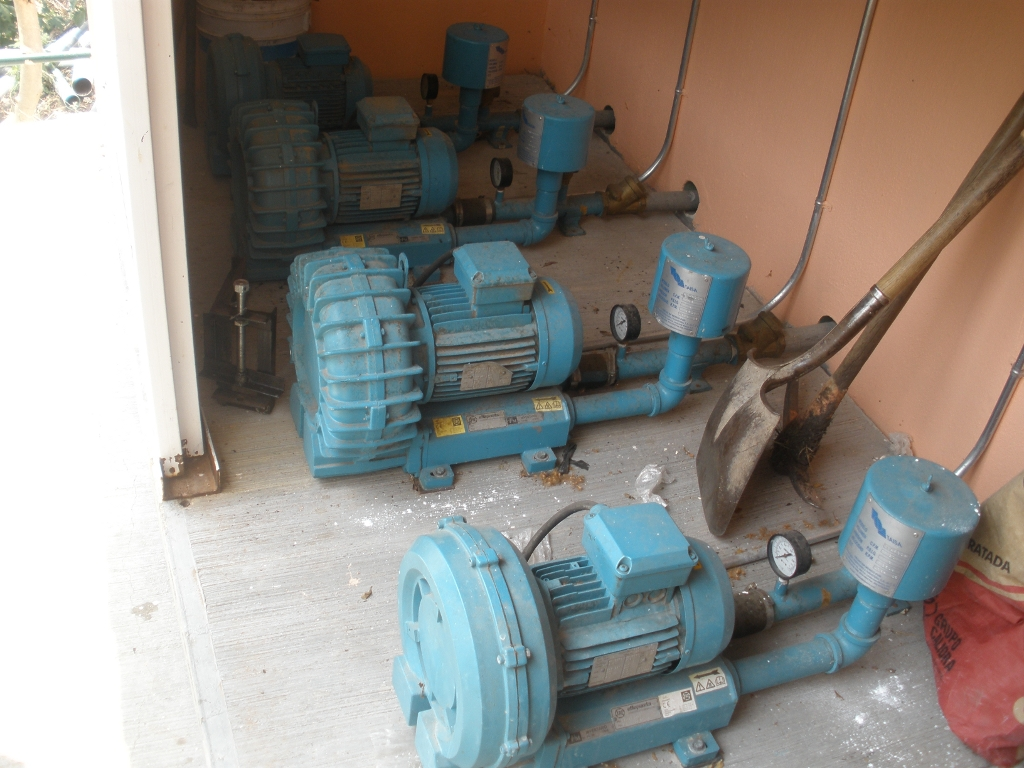
\includegraphics[scale=0.2]{Imagenes/MarcoTeorico/Difusores.JPG}
	\end{center}
	\caption{Sistema de difusores.} \label{fig:cap2:PTAR:Dif}
\end{figure}

%-------------------------------------------------------------------
\section{Descripci�n de sensores}
%-------------------------------------------------------------------
\label{cap2:sec:Sensores}

\subsection{Electrodo de pH}
\label{cap2:Sensores:pH}

Los electrodos de pH se usan en una gran variedad de aplicaciones incluyendo el tratamiento de aguas, procesos qu�micos, instrumentaci�n m�dica y sistemas de evaluaci�n ambiental \cite{Cap2Bib:PHElectrode}.%Designing with pH Electrodes

En este trabajo de tesis se utiliza un electrodo para medici�n de pH de la marca \emph{Cole Parmer}, cuyo modelo es \emph{EW-05992-10}. Esta marca maneja dos tipos de electrodos, uno de uni�n simple y otro de uni�n doble. En este caso se ha usado el de uni�n doble, como el que se ilustra en la figura~\ref{fig:cap2:sec:Sensores:pH1}.

\begin{figure}[htb]
	\begin{center}
		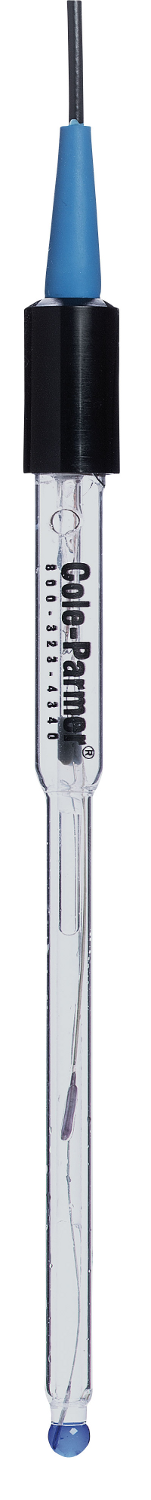
\includegraphics[scale=0.3,angle=90]{Imagenes/MarcoTeorico/ElectrodopH.png}
	\end{center}
	\caption{Electrodo de pH de la marca \emph{Cole Parmer}.}\label{fig:cap2:sec:Sensores:pH1}
\end{figure}

\subsubsection{Principio de funcionamiento del electrodo de pH}
\label{cap2:sec:Sensores:pH:PF}

Un electrodo de pH mide la actividad de iones de hidr�geno ($H^{+}$) y produce un potencial el�ctrico o voltaje. La operaci�n del electrodo de pH est� basada en el principio de que un potencial el�ctrico se genera cuando dos l�quidos con diferente pH entran en contacto en los lados opuestos de una membrana delgada de cristal \cite{Cap2Bib:PHElectrode}.

Los electrodos de pH modernos son una combinaci�n de electrodos compuestos de dos partes principales, un electrodo cristal y un electrodo de referencia como se ilustra en la figura~\ref{fig:cap2:sec:Sensores:pH2}. El pH es determinado esencialmente a trav�s de la medici�n de la diferencia de voltaje entre estos dos electrodos.

\begin{figure}[htb]
	\begin{center}
		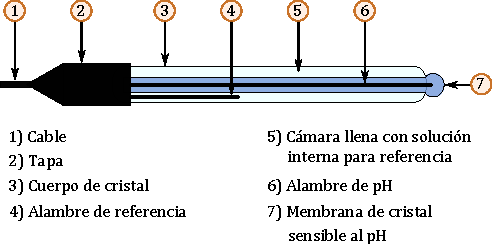
\includegraphics[scale=0.9]{Imagenes/MarcoTeorico/ElectrodopH.pdf}
	\end{center}
	\caption{Caracter�sticas del electrodo de pH.}\label{fig:cap2:sec:Sensores:pH2}
\end{figure}

En la punta del electrodo se encuentra la membrana peque�a, la cual es un tipo de cristal espec�fico capaz de intercambiar iones. �ste es el elemento que sensa la concentraci�n de hidr�geno de la soluci�n de prueba. El potencial del electrodo de referencia es constante y es producido por el elemento interno del mismo, ya que se encuentra en contacto con la soluci�n de relleno de referencia, la cual tiene un pH constante con un valor de siete.

\subsubsection{Caracter�sticas del electrodo de pH}
\label{cap2:sec:Sensores:pH:Ca}

Los electrodos de pH son sensores activos, lo que significa que no requieren de una fuente de excitaci�n o polarizaci�n (voltaje o corriente) externa. Este electrodo se clasifica como un sensor bipolar debido a que la salida del electrodo puede oscilar por arriba o por abajo del punto de referencia. El electrodo produce un voltaje de salida, el cual es linealmente proporcional al valor de pH de la soluci�n que est� siendo medida. El rango de valores de pH en que opera el electrodo es de 0 a 14 \cite{Cap2Bib:PHElectrode}.

La impedancia de salida en este electrodo de pH es muy alta, esto se debe a que el bulbo de cristal tiene una resistencia que t�picamente se encuentra en el rango de $10 - 1000\mega\ohm$. Esto significa que el electrodo solamente puede ser monitoreado por un dispositivo de medici�n con una impedancia de entrada muy alta.

Las funciones de transferencia mostradas en la figura~\ref{fig:cap2:sec:Sensores:pH3} y la figura ~\ref{fig:cap2:sec:Sensores:pH4} indican que cuando el pH de la soluci�n incrementa, el voltaje producido por el electrodo de pH decrementa. Como se observa en la figura~\ref{fig:cap2:sec:Sensores:pH3}, la sensibilidad del electrodo de pH var�a con respecto a la temperatura.

\begin{center}
	\pgfplotsset{every axis/.append style={thick,tick style={thin},font=\footnotesize}}

\begin{tikzpicture}
\tikzset{
every pin/.style={fill=yellow!50!white,rectangle,rounded corners=3pt,font=\scriptsize},
small dot/.style={fill=black,circle,scale=0.3}
}
	\begin{axis}[use units,x=.4cm,y=6cm,
		minor tick num=3,
		axis y line=left,
		axis x line=middle,
		x unit=pH,
		y unit=V, y unit prefix=m,ylabel=Salida
				]

	\addplot[smooth,teal,mark=none,domain=0:14,samples=40]
		%{sin(deg(x))};
		{(x-7)*-0.05916};
	\addplot[smooth,orange,mark=none,domain=0:14,samples=40]
		%{sin(deg(x))};
		{(x-7)*-0.07004};
	\addplot[smooth,blue,mark=none,domain=0:14,samples=40]
		%{sin(deg(x))};
		{(x-7)*-0.05420};

\node[small dot,pin=0:{$100\:\degreecelsius$ $(70.04\:\milli\volt\per pH)$}] at (axis description cs:0.06,.94) {};
\node[small dot,pin=3:{$25\:\degreecelsius$ $(59.16\:\milli\volt\per pH))$}] at (axis description cs:.205,.75) {};
\node[small dot,pin=200:{$0\:\degreecelsius$ $(54.20\:\milli\volt\per pH))$}] at (axis description cs:.76,0.3) {};
	\end{axis}
	
	
\end{tikzpicture}



	\captionof{figure}{Funci�n de transferencia del electrodo de pH.} \label{fig:cap2:sec:Sensores:pH3}
\end{center}

El electrodo ideal a una temperatura de $25\degreecelsius$ tiene una sensibilidad de $59.16\milli\volt \per pH$, lo que significa que la se�al de salida del electrodo oscila de $+414.12\milli\volt$ a $-414.12\milli\volt$ para el rango de pH entre $0$ y $14$ respectivamente.

\begin{figure}[htb]
	\begin{center}
		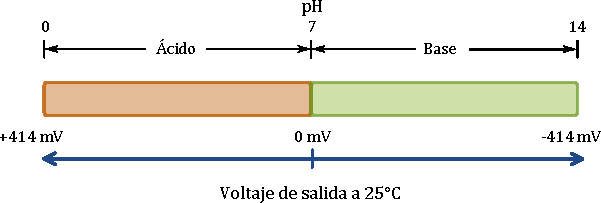
\includegraphics[scale=0.9]{Imagenes/MarcoTeorico/pHTF.pdf}
	\end{center}
	\caption{Voltaje de salida del sensor en funci�n del nivel de pH.} \label{fig:cap2:sec:Sensores:pH4}
\end{figure}

\subsection{Electrodo de ox�geno disuelto}
\label{cap2:sec:Sensores:OD}

Existen dos principales tipos de electrodos de ox�geno disuelto (OD): electrodos sin membrana y electrodos con membrana permeable (\emph{Principio de Clark}) \cite{Cap2Bib:OD}.

Actualmente los electrodos con membrana que funcionan con el principio de Clark son los m�s usados globalmente, los cuales permiten mediciones de ox�geno en gases y soluciones, otra ventaja es que el electrodo y la soluci�n no se contaminan mutuamente.

En la UTM se cuenta con un electrodo de OD marca \emph{Mettler-Toledo}, cuyo modelo es \emph{InPro 6800} como el que se muestra en la figura~\ref{fig:cap2:sec:Sensores:OD1}. Este electrodo est� destinado a mediciones en l�nea (\emph{Inline Measurement}) de la presi�n parcial de ox�geno en l�quidos y gases .

\begin{figure}[htb]
	\begin{center}
		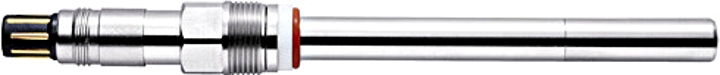
\includegraphics[scale=0.4]{Imagenes/MarcoTeorico/DOElectrode.png}
	\end{center}
	\caption{Electrodo de ox�geno disuelto de la marca \emph{Mettler Toledo}.}\label{fig:cap2:sec:Sensores:OD1}
\end{figure}

Algunas de las aplicaciones de estos electrodos de OD son: fermentaci�n, propagaci�n de levadura, aireaci�n de mosto, acondicionamiento de agua de manantial y almacenamiento y procesado de jugo de frutas.

\subsubsection{Principio de funcionamiento del electrodo de ox�geno disuelto}
\label{cap2:sec:Sensores:OD:PF}

El electrodo \emph{InPro 6800} est� basado en el principio de medici�n polarogr�fica (\emph{Clark Polarographic Sensor}), el cual consiste de un electrodo de operaci�n (\emph{c�todo}), un electrodo de contra-referencia (\emph{�nodo}) y una membrana permeable al ox�geno, dicha membrana separa los electrodos de la muestra. En la figura~\ref{fig:cap2:sec:Sensores:OD2} se ilustran los componentes del electrodo de ox�geno disuelto \cite{Cap2Bib:OD}.

\begin{figure}[htb]
	\begin{center}
		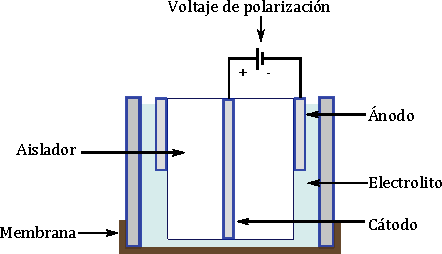
\includegraphics[scale=0.9]{Imagenes/MarcoTeorico/ElectrodoOD.pdf}
	\end{center}
	\caption{Caracter�sticas del electrodo de ox�geno disuelto.} \label{fig:cap2:sec:Sensores:OD2}
\end{figure}


El electrodo de OD es un sensor pasivo, lo que quiere decir que requiere una fuente de excitaci�n, en este caso se le llama fuente de polarizaci�n. Esta fuente de polarizaci�n debe proporcionar un voltaje constante al c�todo para reducir el ox�geno. 

Las mol�culas de ox�geno que migran a trav�s de la membrana permeable son reducidas en el c�todo. Al mismo tiempo se origina una oxidaci�n en el �nodo, por lo que el metal (\emph{Plata}) oxidado del �nodo es liberado en forma de iones de plata dentro de un electrolito. El electrolito provoca que se cierre el circuito el�ctrico entre el �nodo y el c�todo (conductividad i�nica).

La corriente producida por las reacciones descritas anteriormente es proporcional a la presi�n parcial del ox�geno en la muestra.

\subsubsection{Caracter�sticas del electrodo de ox�geno disuelto}
\label{cap2:sec:Sensores:OD:Ca}

Para un funcionamiento correcto, el electrodo \emph{InPro 6800} requiere de una polarizaci�n completa, lo cual se logra cuando se mantiene conectado el electrodo al voltaje de polarizaci�n constantemente por $6$ horas. Si el sensor es desconectado por m�s de 5 minutos, se debe volver a realizar el proceso de polarizaci�n \cite{Cap2Bib:OD}.

En aplicaciones est�ndares, como en este caso, el voltaje de polarizaci�n debe ser de $675\milli\volt$ y debe permanecer constante. La se�al de salida del sensor de OD oscila de $50\nano\ampere$ a $110\nano\ampere$ al aire ambiente.

El rango de temperatura para una correcta operaci�n es de $0-80\degreecelsius$. El rango de operaci�n del electrodo es de $0$ppm a $60$ppm (ppm, \emph{partes por mill�n}). La precisi�n que proporciona es menor o igual a $1\%+6$ppm para lecturas en l�quidos. El material con el que est� construido el c�todo es platino (\emph{Pt}) y el �nodo es de plata (\emph{Ag}).

\subsection{Sensor de temperatura LM35}
\label{cap2:sec:Sensores:Temp}

El sensor de circuito integrado \emph{LM35} es un sensor de temperatura de precisi�n, el cual es un sensor pasivo cuyo voltaje de salida es linealmente proporcional a la temperatura en grados cent�grados ($\degreecelsius$). En la figura~\ref{fig:cap2:sec:Sensores:Temp1} se ilustra el encapsulado y la configuraci�n del sensor \cite{Cap2Bib:LM35}.

\begin{figure}[htb]
	\begin{center}
		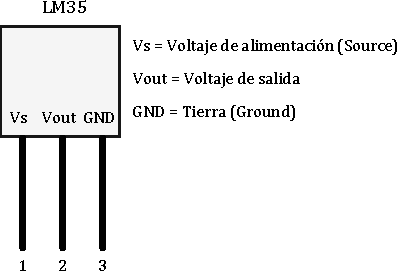
\includegraphics[scale=0.9]{Imagenes/MarcoTeorico/LM35.pdf}
	\end{center}
	\caption{Configuraci�n del sensor LM35.} \label{fig:cap2:sec:Sensores:Temp1}
\end{figure}

\subsubsection{Funcionamiento y caracter�sticas del sensor LM35}
\label{cap2:sec:Sensores:Temp:PFCa}

El voltaje de operaci�n del sensor \emph{LM35} es de $4$ a $30\volt$, tiene un rango de operaci�n de $-55$ a $150\degreecelsius$ y tiene una sensibilidad de $10\milli\volt \per \degreecelsius$. El LM35 no requiere de una calibraci�n externa y proporciona una precisi�n de $\pm0.25\milli\volt$ \cite{Cap2Bib:LM35}.

La impedancia de salida del LM35 es baja, adem�s permite el uso de una fuente individual de excitaci�n, lo que facilita el dise�o del circuito electr�nico de interfaz.

%-------------------------------------------------------------------------------
\section{Protocolos de comunicaciones}
%-------------------------------------------------------------------------------
\label{cap2:sec:Protocolos}

Un protocolo de comunicaciones es un conjunto de reglas y convenciones que deben seguir dos equipos cualesquiera (computadoras o dispositivos) para intercambiar informaci�n a trav�s de una red. Un protocolo es una regla o est�ndar que controla o permite la comunicaci�n en su forma m�s simple. Puede ser definido como las reglas que dominan la sintaxis, sem�ntica y sincronizaci�n de la comunicaci�n. Puede ser implementado por \emph{hardware}, \emph{software} o una combinaci�n de ambos \cite{Cap2Bib:Cisco, Cap2Bib:NetworkProtocols, Cap2Bib:ProtocolEngineering}.

Cualquier red de comunicaciones de datos requiere un sistema para organizar el flujo de datos. Para ordenar los protocolos de comunicaciones, la Organizaci�n Internacional de Est�ndares (ISO, \emph{International Organization for Standarization}), propuso en el a�o de 1984 el modelo de referencia para la Interconexi�n de Sistemas Abiertos (OSI, \emph{Open System Interconnection}) \cite{Cap2Bib:Cisco, Cap2Bib:NetworkProtocols, Cap2Bib:ProtocolEngineering}.

El modelo OSI describe las reglas que los equipos de comunicaciones deben seguir para que el intercambio de datos sea posible dentro de una infraestructura que est� compuesta por una gran variedad de productos de diferentes fabricantes \cite{Cap2Bib:Cisco}.

\subsection{El modelo de referencia OSI}

Las recomendaciones del modelo OSI no son normas concretas, sino reglas gen�ricas para separar en siete niveles, o capas, el proceso de comunicaci�n entre dos sistemas. Las capas del modelo OSI son (figura~\ref{fig:cap2:PC:OSI}): f�sica, enlace de datos, red, transporte, sesi�n, presentaci�n y aplicaci�n \cite{Cap2Bib:Cisco, Cap2Bib:NetworkProtocols, Cap2Bib:ProtocolEngineering}.

El modelo OSI permite que cada nivel se encargue de tareas espec�ficas y utilice los servicios de los niveles inferiores sin preocuparse de c�mo funcionan. Por lo que resulta f�cil realizar cambios en una parte sin tener que alterar el resto de las especificaciones. La comunicaci�n entre dos sistemas solo puede realizarse entre capas del mismo nivel, en la figura~\ref{fig:cap2:PC:OSI} se muestra el flujo de datos entre capas de dos sistemas que se comunican empleando el modelo de referencia OSI.

\begin{figure}[htb]
	\begin{center}
		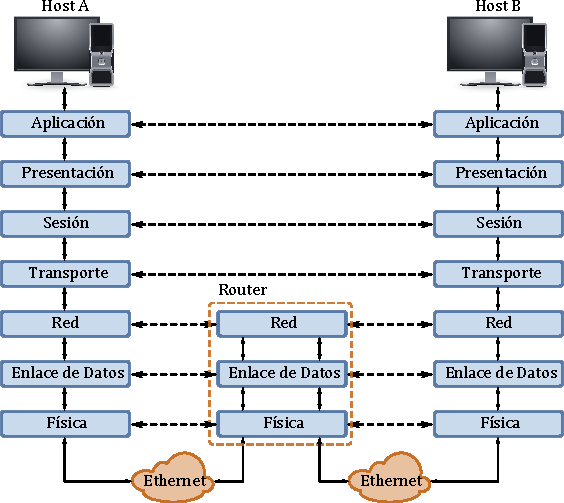
\includegraphics[scale=0.9]{Imagenes/MarcoTeorico/OSIComm.pdf}
	\end{center}
	\caption{Arquitectura de protocolos del modelo de referencia OSI.} \label{fig:cap2:PC:OSI}
\end{figure}

\subsubsection{Capa f�sica}

En la capa f�sica se especifican las caracter�sticas mec�nicas y el�ctricas del sistema f�sico de transporte (par trenzado, coaxial, fibra �ptica, etc.) y de las interfaces que permiten la conexi�n f�sica de los equipos a dichos sistemas de transporte \cite{Cap2Bib:Cisco, Cap2Bib:NetworkProtocols, Cap2Bib:ProtocolEngineering}.

En este nivel se definen las topolog�as aceptadas, el modo de emisi�n o forma de la se�al y el soporte de transmisi�n (banda base o se�al portadora).

Las caracter�sticas de las se�ales y conexiones que se definen son: caracter�sticas f�sicas de los conectores, caracter�sticas el�ctricas de las se�ales (voltaje e impedancia), caracter�sticas el�ctricas del \emph{hardware}, implementaci�n de las se�ales y la codificaci�n.

El objetivo primordial de la capa f�sica consiste en transmitir bits por un canal de comunicaci�n, de manera que todo lo que env�e el transmisor llegue al receptor sin sufrir alteraciones.

Globalmente las interfaces de capa f�sica para comunicaciones de datos incluyen interfaces serie como \emph{EIA/TIA-232} y \emph{EIA/TIA-485}, interfaces paralelas, y las especificaciones f�sicas para sistemas LAN tales como \emph{Ethernet} (figura~\ref{fig:cap2:PC:OSI}) y \emph{Token Ring}. Los sistemas inal�mbricos cuentan con interfaces a�reas que definen la transmisi�n de datos usando radio, microondas o se�ales infrarrojas.

\subsubsection{Capa de enlace de datos}

La capa de enlace de datos define las reglas para enviar y recibir informaci�n a trav�s de una conexi�n f�sica entre dos sistemas. Establece la forma de agrupar los datos en paquetes o tramas de longitud adecuada y a�ade los mecanismos necesarios para controlar la transmisi�n de informaci�n y detectar y corregir los errores que puedan aparecer \cite{Cap2Bib:Cisco, Cap2Bib:NetworkProtocols, Cap2Bib:ProtocolEngineering}.

El acceso al medio f�sico puede ser de tres maneras:
\begin{itemize}\itemsep=-0.5em

\item \emph{Controlado por un equipo �nico}: Este sistema emplea la arquitectura Maestro/Esclavo (por ejemplo el protocolo Modbus).

\item \emph{Condicionado por un derecho}: En este sistema el derecho de acceso es proporcionado por un testigo, el equipo que tiene dicho testigo puede emitir un mensaje y transmitir el testigo al siguiente equipo (por ejemplo el protocolo Profibus).

\item \emph{Aleatorio o descentralizado}: El equipo que quiere emitir verifica que la l�nea de transmisi�n est� libre. Si dos equipos emiten de forma simult�nea, se origina una colisi�n y ambos mensajes se destruyen. Tal es el caso de los protocolos del tipo CSMA (\emph{Carrier Sense Multiple Access}) empleados principalmente en redes Ethernet.
\end{itemize}

\subsubsection{Capa de red}

Esta capa provee servicios de interconexi�n de redes para la distribuci�n de datos a trav�s de m�ltiples redes. La capa de red se ocupa del direccionamiento a trav�s de sistemas mediante t�cnicas de encaminamiento (ruteo, \emph{Routing}) y el control de flujo. El esquema de direccionamiento de redes asigna una direcci�n �nica a cada red y a cada equipo conectado \cite{Cap2Bib:Cisco, Cap2Bib:NetworkProtocols, Cap2Bib:ProtocolEngineering}.

El protocolo IP dentro de la suite de protocolos TPC/IP, es un ejemplo de protocolo de capa de red.

\subsubsection{Capa de transporte}

La capa de transporte provee servicios de comunicaciones entre dos sistemas. Tiene la funci�n de garantizar un enlace fiable asegurando que los datos sean entregados. Ambos sistemas establecen una conexi�n y mantienen un di�logo para llevar el control de la entrega de paquetes a trav�s de la red \cite{Cap2Bib:Cisco, Cap2Bib:NetworkProtocols, Cap2Bib:ProtocolEngineering}.

Un protocolo de la capa de transporte divide la informaci�n en paquetes manejables por el sistema de transmisi�n y controla la gesti�n de paquetes (orden de env�o y recepci�n, formatos de transmisi�n, peticiones de reenv�o en caso de error, etc.).

\subsubsection{Capa de sesi�n}

La capa de sesi�n establece, administra y termina las sesiones de comunicaci�n entre equipos. Las sesiones de comunicaci�n consisten de peticiones y respuestas de servicio, las cuales se llevan a cabo entre aplicaciones de diferentes equipos en la red \cite{Cap2Bib:Cisco, Cap2Bib:NetworkProtocols, Cap2Bib:ProtocolEngineering}.

\subsubsection{Capa de presentaci�n}

La capa de presentaci�n provee una variedad de funciones de codificaci�n y conversi�n que son aplicados a los datos de la capa de aplicaci�n. Estas funciones aseguran que la informaci�n enviada desde la capa de aplicaci�n de un sistema sea entendible por la capa de aplicaci�n de otro sistema \cite{Cap2Bib:Cisco, Cap2Bib:NetworkProtocols, Cap2Bib:ProtocolEngineering}.

\subsubsection{Capa de aplicaci�n}

La capa de aplicaci�n es la m�s cercana al usuario final, por lo tanto, el usuario final y la capa de aplicaci�n interact�an directamente con el \emph{software} de aplicaci�n \cite{Cap2Bib:Cisco, Cap2Bib:NetworkProtocols, Cap2Bib:ProtocolEngineering}.

Esta capa es un espacio de libre utilizaci�n para fabricantes y usuarios. Presta servicios al usuario, los cuales comprenden la interacci�n directa con los procesos de aplicaci�n. Algunos ejemplos de implementaciones en la capa de aplicaci�n incluyen Telnet, el protocolo de transferencia de ficheros (FTP, \emph{File Transfer Protocol}), bases de datos y el protocolo de transferencia de correo simple (SMTP, \emph{Simple Mail Transfer Protocol}).

\subsection{Interfaces serie}

En las comunicaciones del entorno industrial, las conexiones f�sicas se realizan mediante interfaces serie, las cuales son normalizadas por la Asociaci�n de Industrias Electr�nicas (EIA, \emph{Electronic Industrial Asociation}) y la Asociaci�n de la Industria de Telecomunicaciones (TIA, \emph{Telecommunications Industry Association}) \cite{Cap2Bib:PracticalScada,  Cap2Bib:CommEmpresa, Cap2Bib:DataCommunications}.

Los est�ndares de interfaces serie m�s conocidos son: \emph{EIA/TIA-232} o \emph{RS-232}, y \emph{EIA/TIA-485} o \emph{RS-485}. Los cuales forman el elemento principal para la transferencia de informaci�n digital entre una RTU y un m�dem (modulador/demodulador). El m�dem es aquel que convierte las se�ales digitales (TTL), generadas por una computadora o un sistema basado en MCU, en una forma anal�gica adecuada para la transmisi�n a distancias grandes a trav�s de cables o un sistema de radio.

En los est�ndares RS-232 y RS-485 se definen las caracter�sticas el�ctricas y los detalles mec�nicos que permiten a equipos de comunicaciones, de diferentes fabricantes, conectarse y funcionar eficientemente.

\subsubsection{Comunicaci�n de datos serie en el est�ndar RS-232}

El est�ndar de interfaz RS-232 define la interfaz entre un Equipo Terminal de Datos (DTE, \emph{Data Terminal Equipment}) y un Equipo de Comunicaciones de Datos (DCE, \emph{Data Communication Equipment}) empleando el intercambio de datos binarios serie, en donde el DCE es el dispositivo que emite datos y el DTE es que recibe dichos datos \cite{Cap2Bib:PracticalScada, Cap2Bib:CommEmpresa, Cap2Bib:DataCommunications}.

El est�ndar RS-232 consiste principalmente de tres partes, las cuales definen las caracter�sticas de las se�ales el�ctricas, las caracter�sticas de la interfaz mec�nica y la descripci�n funcional de los circuitos de intercambio.

Los conectores com�nmente asociados al est�ndar RS-232 son el DB-25 (tipo D de 25 pines) y el DB-9 (tipo D de 9 pines) \cite{Cap2Bib:CommEmpresa}, de los cuales el conector DB-9 es el m�s usado globalmente en computadoras y dispositivos en el �mbito industrial. En la figura~\ref{fig:cap2:PC:DB9} se muestra la asignaci�n de terminales y las se�ales del conector DB-9 del est�ndar RS-232.

\begin{figure}[htb]
	\begin{center}
		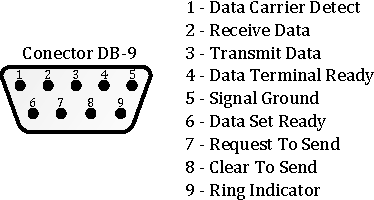
\includegraphics[scale=0.9]{Imagenes/MarcoTeorico/DB-9.pdf}
	\end{center}
	\caption{Asignaci�n de terminales y se�ales del conector DB-9 para el est�ndar RS-232.} \label{fig:cap2:PC:DB9}
\end{figure}

\paragraph{Caracter�sticas de las se�ales el�ctricas}

El est�ndar de interfaz RS-232 est� dise�ado para la comunicaci�n de dispositivos DTE y DCE, en donde un dispositivo DTE es aquel que transmite los datos y un dispositivo DCE es aquel que los recibe \cite{Cap2Bib:PracticalScada, Cap2Bib:CommEmpresa, Cap2Bib:DataCommunications}.

Para un receptor RS-232, las especificaciones de los niveles de voltaje se describen en la tabla~\ref{tab:cap01:PC:RS232}.

\begin{table}[htb]
	\caption{Niveles de voltaje del receptor del est�ndar RS-232.}%
	\centering
	\footnotesize
	\begin{tabular}{ll}
		\hline \hline \hline \hline
		\headcol \textbf{Estados l�gicos} & \textbf{Niveles de voltaje} \\ 
		\hline \hline \hline \hline

		Estado L�gico 0 	& $+3\volt$ a $+25\volt$\\
		\rowcol Estado L�gico 1 	& $-3\volt$ a $-25\volt$\\
		Estado Indefinido	& $-3\volt$ a $+3\volt$\\

		\hline \hline	\hline \hline 	 		
	\end{tabular}
	\label{tab:cap01:PC:RS232}
\end{table}

De manera similar al receptor, el transmisor RS-232 debe producir niveles de voltaje ligeramente m�s elevados para contrarrestar las ca�das de voltaje a lo largo de la l�nea de transmisi�n (tabla~\ref{tab:cap01:PC:RS232-2}).

\begin{table}[htb]
	\caption{Niveles de voltaje del transmisor del est�ndar RS-232.}%
	\centering
	\footnotesize
	\begin{tabular}{ll}
		\hline \hline \hline \hline
		\headcol \textbf{Estados l�gicos}&\textbf{Niveles de voltaje}\\
		\hline \hline \hline \hline
		Estado L�gico 0 	& $+5\volt$ a $+25\volt$\\
		\rowcol Estado L�gico 1 	& $-5\volt$ a $-25\volt$\\
		\hline \hline \hline \hline
	\end{tabular}
	\label{tab:cap01:PC:RS232-2}
\end{table}

\paragraph{Descripci�n funcional de los circuitos de intercambio}

Las funciones de los circuitos de intercambio definidos en el est�ndar RS-232, son las conexiones o se�ales el�ctricas involucradas en la comunicaci�n, las cuales se describen en la tabla~\ref{tab:cap01:PC:RS232-3} \cite{Cap2Bib:PracticalScada, Cap2Bib:CommEmpresa, Cap2Bib:DataCommunications}.

\begin{table}[htb]
	\caption{Se�ales del est�ndar RS-232.}%
	\centering
	\footnotesize
	\begin{tabular}{lll}
		\hline \hline \hline \hline
		\headcol \textbf{Se�al}&\textbf{Nombre completo}&\textbf{Descripci�n}\\
		\hline \hline \hline \hline
		Common	&	Signal Ground	&	Es la l�nea com�n de referencia.\\
		\rowcol TXD	&	Transmit Data	&	Es la portadora de datos serie de un DTE a un DCE.\\
		RXD	&	Received Data	&	Es la portadora de datos serie de un DCE a un DTE.\\
		\rowcol RTS	&	Request to Send	&	Esta l�nea habilita la transmisi�n.\\
		CTS	&	Clear to Send	&	Es la se�al de inicializacion para enviar.\\
		\rowcol DSR	&	Data Set Ready	&	Indica que el DCE est� listo para recibir.\\
		DCD	&	Data Carrier Detect	&	Detecta la se�al de la l�nea de entrada.\\
		\rowcol DTR	&	Data Terminal Ready	&	Indica que el DTE est� listo para enviar.\\
		\hline \hline \hline \hline
	\end{tabular}
	\label{tab:cap01:PC:RS232-3}
\end{table}

\subsubsection{Comunicaci�n de datos serie en el est�ndar RS-485}
\label{cap2:PC:RS-485}
El est�ndar RS-485 es una expansi�n del est�ndar RS-422, es un m�todo de comunicaci�n usado en aplicaciones industriales. El est�ndar RS-485 define una interfaz de comunicaci�n de datos balanceado o diferencial, haciendo uso de dos cables separados para cada se�al. Esto permite velocidades de transferencia de datos muy elevadas y minimiza los problemas de las variaciones de potencial en la tierra (ground, GND), a diferencia del est�ndar RS-232, la tierra no es usada como voltaje de referencia \cite{Cap2Bib:PracticalScada, Cap2Bib:CommEmpresa, Cap2Bib:DataCommunications}.

El est�ndar RS-485 permite una conexi�n de red multipuntos en dos alambres y una comunicaci�n de datos serie confiable con las siguientes caracter�sticas: una distancia m�xima de alcance de $1200\meter$, una tasa m�xima de transferencia de datos de 10 Mbps (megabits por segundo), permite la conexi�n de 32 transmisores de l�nea (line driver) y 32 receptores de l�nea (line receiver) como m�ximo en la misma l�nea.

Los rangos de voltaje en la l�nea son: $-1.5\volt$ a $-6.0\volt$ para el estado l�gico ``1'', y $+1.5\volt$ a $+6.0\volt$ para el estado l�gico ``0''. Los puntos de referencia usados para estos voltajes son las terminales A y B de los transmisores/receptores de l�nea mostrados en la figura~\ref{fig:cap2:PC:rs485}. El transmisor de l�nea, para una interfaz RS-485, produce un voltaje diferencial de $\pm5\volt$ en los dos alambres.

La mejora m�s importante del est�ndar RS-485 con respecto al est�ndar RS-232 es que el modo de operaci�n del transmisor de l�nea consiste de 3 estados: estado l�gico ``0'', estado l�gico ``1'' y ``alta impedancia''. Dichos estados se definen de la siguiente manera:

\begin{itemize}\itemsep=-0.5em

\item Cuando la terminal A del driver es negativa, con respecto a la terminal B, la l�nea est� en el estado l�gico 1.

\item Cuando la terminal A del driver es positiva, con respecto a la terminal B, la l�nea est� en el estado l�gico 0. 

\item El estado de alta impedancia, tambi�n conocido como estado deshabilitado, puede ser iniciado por una se�al en una terminal de control en el circuito integrado del transmisor de l�nea.

\end{itemize}

Para sistemas \emph{full-duplex} se requiere de cinco alambres, en cambio para sistemas \emph{half-duplex}, solo se requieren tres alambres. En la figura~\ref{fig:cap2:PC:rs485} se ilustra un ejemplo de configuraci�n del est�ndar de interfaz RS-485 multipunto \cite{Cap2Bib:CommEmpresa}.

\begin{figure}[htb]
	\begin{center}
		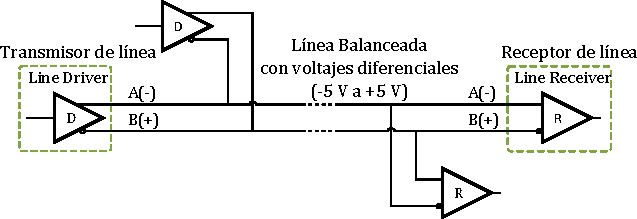
\includegraphics[scale=0.9]{Imagenes/MarcoTeorico/RS-485Multipunto2.pdf}
	\end{center}
	\caption{Interfaz multipunto del est�ndar RS-485.} \label{fig:cap2:PC:rs485}
\end{figure}

Los receptores de l�nea, solamente son sensitivos a la diferencia entre dos se�ales de entrada, por lo que, las se�ales comunes de ruido se presentan en ambos alambres y solamente tendr�n un peque�o efecto en la operaci�n del receptor.

El est�ndar de interfaz RS-485 es �til en sistemas que requieren la conexi�n de m�ltiples dispositivos separados por distancias grandes haciendo uso del mismo par de l�neas. En dichos sistemas se requiere un \emph{software} de control para establecer qu� dispositivo de la red puede estar activo. En la mayor�a de los casos una MTU controla qu� transmisor/receptor estar� activo en alg�n momento.

\subsection{Modbus}

Modbus es un protocolo de comunicaciones clasificado como bus de campo. Un bus de campo es un bus de transferencia de informaci�n en serie utilizado en la industria. Los buses de campo est�n orientados a procesos discretos (autom�viles, electrodom�sticos, etc.) y procesos continuos (petroqu�micas, electricidad, agua, etc.) \cite{Cap2Bib:CommEmpresa, Cap2Bib:DataCommunications, Cap2Bib:IndustrialCT}.

Seg�n la definici�n de la Comisi�n Electrot�cnica Internacional (IEC, \emph{International Electrotechnical Commision}) y la Sociedad de Instrumentaci�n de Am�rica (ISA, \emph{Instrument Society of America}), un bus de campo es una conexi�n serie digital que permite la transferencia de datos entre elementos primarios de automatizaci�n (instrumentos de campo), que realizan funciones de medida y control, y elementos de automatizaci�n y control de m�s alto nivel.

Un bus de campo, al igual que una red LAN, satisface los dos primeros niveles del modelo OSI y el �ltimo (figura~\ref{fig:cap2:PC:MB}). No obstante presenta mensajes m�s cortos (�rdenes, eventos, medidas, etc.), con tiempos de respuesta entre $5\milli\second$ y $100\milli\second$ y alta seguridad en la comunicaci�n, sobre distancias entre $200\meter$ y $2\kilo\meter$, a velocidades que suelen ser inferiores a $1\mega$bps.

Normalmente en el medio f�sico de un bus de campo de bajo costo, consiste de un par de hilos con una interfaz serie RS-485, aunque se encuentran aplicaciones con coaxial, fibra �ptica, radio e infrarrojos.

El est�ndar Modbus define un protocolo de mensajes de la capa de aplicaci�n, posicionado en el nivel siete del modelo OSI, que provee comunicaciones con arquitectura cliente/servidor entre dispositivos conectados en diferentes tipos de buses o redes \cite{Cap2Bib:Modbus1, Cap2Bib:Modbus3, Cap2Bib:Modbus2}. El est�ndar Modbus define un protocolo espec�fico para interfaz serie (Modbus sobre una l�nea serie) para el intercambio de peticiones Modbus haciendo uso de la arquitectura Maestro/Esclavo. En la figura~\ref{fig:cap2:PC:MB} se ilustra el protocolo Modbus con respecto al modelo de referencia OSI \cite{Cap2Bib:Modbus2}.

\begin{figure}[htb]
	\begin{center}
		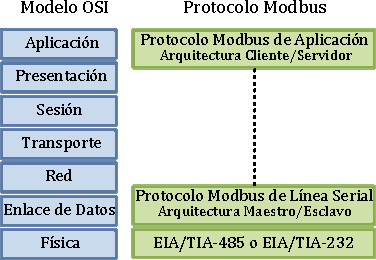
\includegraphics[scale=0.9]{Imagenes/MarcoTeorico/ModeloOSI-Modbus.pdf}
	\end{center}
	\caption{Protocolo Modbus relacionado con el Modelo OSI.} \label{fig:cap2:PC:MB}
\end{figure}

En la actualidad, el protocolo Modbus, es implementado sobre TCP/IP en redes Ethernet y transmisi�n serie as�ncrona en interfaces f�sicas como RS-485 (Secci�n~\ref{cap2:PC:RS-485}).

\subsubsection{Capa de enlace de datos del protocolo Modbus}

El protocolo Modbus sobre una l�nea serie es un protocolo con arquitectura Maestro/Esclavo posicionado en la capa dos del modelo de referencia OSI (figura~\ref{fig:cap2:PC:MB}) \cite{Cap2Bib:Modbus1, Cap2Bib:Modbus2, Cap2Bib:DataCommunications}.

Los principios generales de la comunicaci�n Modbus son: solo un nodo Maestro debe estar conectado al bus o red y un m�ximo de 247 nodos Esclavos, el nodo Maestro iniciar� la comunicaci�n, los nodos Esclavos no transmitir�n datos sin haber recibido una petici�n del nodo Maestro, los nodos Esclavos no se comunicar�n entre ellos y el nodo Maestro mantendr� comunicaci�n con un solo nodo Esclavo a la vez.

El nodo Maestro puede emitir peticiones Modbus de dos modos:
\begin{itemize}\itemsep=-0.5em
\item \emph{Unicast}: Se usa cuando el Maestro se dirige a un nodo Esclavo en espec�fico. El nodo Esclavo, despu�s de recibir e interpretar la petici�n, retornar� un mensaje o respuesta al nodo Maestro.
\item \emph{Broadcast}: En este modo el nodo Maestro manda una petici�n a todos los nodos Esclavo, en este modo no hay una respuesta retornada por los nodos Esclavo.
\end{itemize}

El espacio para direccionamiento del protocolo Modbus comprende 256 diferentes direcciones, las cuales est�n distribuidas de la siguiente manera: la direcci�n 0 est� destinada para peticiones broadcast, por lo que todos los nodos Esclavo deben reconocer esta direcci�n; el nodo Maestro no tiene una direcci�n en particular; los nodos Esclavos tienen una direcci�n �nica en un bus serie, las direcciones de un nodo Esclavo pueden ser desde 1 a 247; las direcciones desde la 248 a la 255 est�n reservadas.

El protocolo Modbus de aplicaci�n define una Unidad de Datos de Protocolo (PDU, Protocol Data Unit) \cite{Cap2Bib:Modbus3}, que se muestra en la figura~\ref{fig:cap2:PC:MB2}, la cual es independiente de las capas inferiores de comunicaci�n (modelo de referencia OSI).

\begin{figure}[htb]
	\begin{center}
		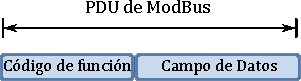
\includegraphics[scale=0.9]{Imagenes/MarcoTeorico/ModbusPDU.pdf}
	\end{center}
	\caption{Unidad de datos de protocolo de MODBUS.} \label{fig:cap2:PC:MB2}
\end{figure}

La implementaci�n del protocolo Modbus sobre una l�nea serie requiere campos adicionales en la PDU (figura~\ref{fig:cap2:PC:MB3}) formando as� una Unidad de Datos de Aplicaci�n (ADU, Application Data Unit) \cite{Cap2Bib:Modbus3}.

\begin{figure}[htb]
	\begin{center}
		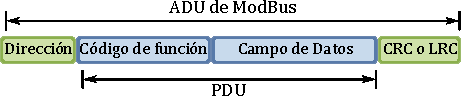
\includegraphics[scale=0.9]{Imagenes/MarcoTeorico/ModbusADU.pdf}
	\end{center}
	\caption{Unidad de datos de aplicaci�n de MODBUS.} \label{fig:cap2:PC:MB3}
\end{figure}

Los campos de la ADU son:

\begin{itemize}\itemsep=-0.5em
\item \emph{Direcci�n}: En el cual el nodo Maestro indica a que nodo Esclavo se dirige y el nodo Esclavo coloca su propia direcci�n para indicar de qu� nodo Esclavo proviene la respuesta.
\item \emph{C�digo de funci�n}: Para indicar al nodo Esclavo que acci�n debe realizar.
\item \emph{Datos}: En donde el nodo Maestro establece los par�metros de la acci�n y el nodo Esclavo coloca la informaci�n o respuesta adecuada a la acci�n solicitada.
\item \emph{Verificaci�n de error}: Es el resultado de un c�lculo de verificaci�n de redundancia realizado sobre el contenido del mensaje o ADU (todos los campos anteriores), para este c�lculo se usan dos tipos de m�todos seg�n sea el modo de transmisi�n: CRC (\emph{Cyclical Redundancy Check}) y LRC (\emph{Longitudinal Redundancy Check}).
\end{itemize}

En Modbus la transmisi�n de ADUs se realizan de dos maneras:
\begin{itemize}\itemsep=-0.5em

\item \emph{RTU}: En donde la codificaci�n es binaria, es decir, cada byte (8-bit) de informaci�n es enviado como dos caracteres de 4 bits hexadecimales. Cada car�cter consta de un bit de inicio, 8 bits de codificaci�n de datos, un bit de paridad (opcional) y uno o dos bits de paro, dando un total de 10 a 12 bits por car�cter. Para la comprobaci�n de errores en las tramas que usan RTU se emplea una secuencia de c�digo CRC.

\item \emph{ASCII}: En el cual la codificaci�n es hexadecimal, es decir, cada byte (8-bit) de informaci�n es enviado como dos caracteres ASCII. Por ejemplo, el byte de 0x5B es codificado como caracteres: 0x35 y 0x42 en c�digo ASCII, en donde 0x35 = ``5'' y 0x42 = ``B''. Cada car�cter consta de un bit de inicio, 7 bits de codificaci�n de datos, un bit de paridad y uno o dos bits de paro, dando un total de 9 a 11 bits por car�cter. Para la comprobaci�n de errores en las ADUs se emplea una secuencia de c�digo LRC.
\end{itemize}

\subsubsection{Descripci�n de los c�digos de funci�n del protocolo Modbus}

Existen tres categor�as de c�digos de funci�n Modbus: c�digos p�blicos, c�digos definidos por el usuario y los c�digos reservados \cite{Cap2Bib:Modbus1, Cap2Bib:Modbus3}. En la tabla~\ref{tab:cap01:PC:Modbus} se muestran los c�digos de funci�n p�blicos que se emplean con mayor frecuencia en equipos y dispositivos conectados en una red serie.

\begin{table}[htb]
	\caption{C�digos de funci�n MODBUS implementados en redes serie.}%
	\centering
	\footnotesize
	\begin{tabular}{ll}
		\hline \hline \hline \hline
		\headcol\textbf{C�digos de Funci�n (hex)}&\textbf{Descripci�n}\\
		\hline \hline \hline \hline
		0x01 & Lectura de Salidas Digitales o Relevadores.\\
		\rowcol 0x02 & Lectura de Entradas Digitales.\\
		0x04 & Lectura de Registros de Entrada.\\
		\rowcol 0x05 & Escritura de una Salida Digital o Relevador Individual.\\		
		0x06 & Escritura de un Registro Individual.\\
		\hline \hline \hline \hline
	\end{tabular}
	\label{tab:cap01:PC:Modbus}
\end{table}

\paragraph{0x01 Lectura de Salidas Digitales o Relevadores}
Este c�digo de funci�n es usado para leer los estados de 1 a 2000 salidas digitales continuas en un dispositivo remoto \cite{Cap2Bib:Modbus1, Cap2Bib:Modbus3}.

La PDU de petici�n (tabla~\ref{tab:MB-Func-01R}) del nodo Maestro especifica los siguientes campos: la direcci�n de la salida digital de inicio, es decir, la direcci�n de la primera salida digital especificada; y, la cantidad de salidas digitales. En la PDU las direcciones de las salidas digitales empiezan desde la direcci�n cero.

\begin{table}[htb]
	\caption{PDU de Petici�n de la funci�n 0x01.}%
	\centering
	\footnotesize
	\begin{tabular}{lll}
		\hline \hline \hline \hline
		\headcol\textbf{C�digo de Funci�n}&\textbf{Direcci�n de Inicio}&\textbf{Cantidad de Salidas}\\
		\hline \hline \hline \hline\hline
		1 Byte			& 2 Bytes			& 2 Bytes \\
		\rowcol \textbf{0x01}		& 0x0000 hasta 0xFFFF		& 1 hasta 2000(0x7D0)\\
		\hline \hline \hline \hline
	\end{tabular}
	\label{tab:MB-Func-01R}
\end{table}

En la PDU de respuesta (tabla~\ref{tab:MB-Func-01A}) del nodo Esclavo, cada estado de una salida digital es representado con un bit en el campo de datos. El estado l�gico ``1'' indica que la salida digital est� habilitada y el estado l�gico ``0'' indica que est� deshabilitada. El bit menos significativo indica el estado correspondiente a la primera salida digital y as� sucesivamente hasta el bit m�s significativo. El campo de cantidad de bytes especifica la cantidad de bytes en el campo de datos.

\begin{table}[htb]
	\caption{PDU de Respuesta de la funci�n 0x01.}%
	\centering
	\footnotesize
	\begin{tabular}{lll}
		\hline \hline \hline \hline
		\headcol\textbf{C�digo de Funci�n}&\textbf{Cantidad de bytes}&\textbf{Array de Estado de Salidas}\\
		\hline \hline \hline \hline\hline
		1 Byte			& 1 Bytes			& n*Bytes \\
		\rowcol \textbf{0x01}		& N bytes			& n=N � n=N+1\\
		\hline \hline \hline \hline\hline
	\end{tabular}
	\label{tab:MB-Func-01A}
\end{table}

\paragraph{0x02 Lectura de Entradas Digitales}
Este c�digo de funci�n es usado para leer los estados de 1 a 2000 entradas digitales continuas en un dispositivo remoto \cite{Cap2Bib:Modbus1, Cap2Bib:Modbus3}.

La PDU de petici�n (tabla~\ref{tab:MB-Func-02Req}) del nodo Maestro especifica los siguientes campos: la direcci�n de la entrada digital de inicio, es decir, la direcci�n de la primera entrada digital especificada; y la cantidad de entradas digitales. En la PDU las direcciones de las entradas digitales empiezan desde la direcci�n cero.

\begin{table}[htb]
	\caption{PDU de Petici�n de la funci�n 0x02.}%
	\centering
	\footnotesize
	\begin{tabular}{lll}
		\hline \hline \hline \hline
		\headcol\textbf{C�digo de Funci�n}&\textbf{Direcci�n de Inicio}&\textbf{Cantidad de Entradas}\\
		\hline \hline \hline \hline
		1 Byte			& 2 Bytes			& 2 Bytes \\
		\rowcol \textbf{0x02}		& 0x0000 hasta 0xFFFF		& 1 hasta 2000(0x7D0)\\
		\hline \hline \hline \hline
	\end{tabular}
	\label{tab:MB-Func-02Req}
\end{table}

En la PDU de respuesta (tabla~\ref{tab:MB-Func-02Res}) del nodo Esclavo, cada estado de una entrada digital es representado con un bit en el campo de datos. El estado l�gico ``1'' indica que la entrada digital est� habilitada y el estado l�gico ``0'' indica que est� deshabilitada. El bit menos significativo indica el estado correspondiente a la primera entrada digital y as� sucesivamente hasta el bit m�s significativo. El campo de cantidad de bytes especifica la cantidad de bytes en el campo de datos.

\begin{table}[htb]
	\caption{PDU de Respuesta de la funci�n 0x02.}%
	\centering
	\footnotesize
	\begin{tabular}{lll}

		\hline \hline \hline \hline
		\headcol\textbf{C�digo de Funci�n}&\textbf{Cantidad de bytes}&\textbf{Array de Estado de Entradas}\\
		\hline \hline \hline \hline
		1 Byte			& 1 Bytes			& n Bytes \\
		\rowcol \textbf{0x02}		& N bytes			& n=N � n=N+1\\
		\hline \hline \hline \hline

	\end{tabular}
	\label{tab:MB-Func-02Res}
\end{table}

\paragraph{0x04 Lectura de Registros de Entrada}
Este c�digo de funci�n es usado para leer los estados de 1 a 125 registros de entrada continuos en un dispositivo remoto \cite{Cap2Bib:Modbus1, Cap2Bib:Modbus3}.

La PDU de petici�n (tabla~\ref{tab:MB-Func-04Req}) del nodo Maestro especifica los siguientes campos: la direcci�n del registro de entrada de inicio, es decir, la direcci�n del primer registro de entrada especificado; y, la cantidad de registros de entradas. En la PDU las direcciones de los registros de entrada empiezan desde la direcci�n cero.

\begin{table}[htb]
	\caption{PDU de Petici�n de la funci�n 0x04.}%
	\centering
	\footnotesize
	\begin{tabular}{lll}
		\hline \hline \hline \hline
		\headcol\textbf{C�digo de Funci�n} 	& \textbf{Direcci�n de Inicio} 	& \textbf{Cantidad de Registros de Entrada}\\
		\hline \hline \hline \hline
		1 Byte			& 2 Bytes			& 2 Bytes \\
		\rowcol \textbf{0x04}		& 0x0000 hasta 0xFFFF		& 0x0001 hasta 0x007D\\
		\hline \hline \hline \hline
	\end{tabular}
	\label{tab:MB-Func-04Req}
\end{table}

En la PDU de respuesta (tabla~\ref{tab:MB-Func-04Res}) del nodo Esclavo, los datos de cada registro de entrada constan de 2 bytes y su contenido binario est� alineado a la derecha. Como cada registro de entrada es de 16 bits separados en 2 bytes, por cada registro, el primer byte contiene los bits de la parte alta y el segundo contiene los bits de la parte baja. El campo de cantidad de bytes especifica la cantidad de bytes en el campo de datos.

\begin{table}[htb]
	\caption{PDU de Respuesta de la funci�n 0x04.}%
	\centering
	\footnotesize
	\begin{tabular}{lll}
		\hline \hline \hline \hline
		\headcol\textbf{C�digo de Funci�n}&\textbf{Cantidad de bytes}&\textbf{Array de Estado de Entradas}\\
		\hline \hline \hline \hline
		1 Byte			& 1 Bytes			& Nx2 Bytes \\
		\rowcol \textbf{0x04}		& 2xN				& \\
		\hline \hline \hline \hline
	\end{tabular}
	\label{tab:MB-Func-04Res}
\end{table}

\paragraph{0x05 Escritura de una Salida Digital o Relevador Individual}
Este c�digo de funci�n es usado para escribir o establecer el estado de una salida digital individual en un dispositivo remoto \cite{Cap2Bib:Modbus1, Cap2Bib:Modbus3}.

En la PDU de petici�n (tabla~\ref{tab:MB-Func-05Req}) del nodo Maestro se especifica la direcci�n de la salida digital individual y el estado (habilitado o deshabilitado) se especifica a trav�s de un valor constante en el campo de datos de la PDU, el valor hexadecimal ``FF 00'' especifica que la salida digital sea habilitada y el valor hexadecimal ``00 00'' especifica que la salida digital sea deshabilitada.

\begin{table}[htb]
	\caption{PDU de la funci�n 0x05.}%
	\centering
	\footnotesize
	\begin{tabular}{lll}
		\hline \hline \hline \hline
		\headcol\textbf{C�digo de Funci�n} 	& \textbf{Direcci�n de la Salida} 	& \textbf{Valor de Salida}\\
		\hline \hline \hline \hline
		1 Byte			& 2 Bytes			& 2 Bytes \\
		\rowcol \textbf{0x05}		& 0x0000 hasta 0xFFFF		& 0x0000 � 0xFF00\\
		\hline \hline \hline \hline
	\end{tabular}
	\label{tab:MB-Func-05Req}
\end{table}

La PDU de respuesta (tabla~\ref{tab:MB-Func-05Req}) del nodo Esclavo es un eco de la PDU de petici�n, la cual usualmente es retornada despu�s de haber establecido el estado de la salida individual.

\paragraph{0x06 Escritura de un Registro Individual}
Este c�digo de funci�n es usado para escribir o establecer un registro individual en un dispositivo remoto \cite{Cap2Bib:Modbus1, Cap2Bib:Modbus3}.

En la PDU de petici�n (tabla~\ref{tab:MB-Func-06Req}) del nodo Maestro, se especifica la direcci�n del registro individual a ser escrito. En la PDU las direcciones de los registros mantenidos empiezan desde la direcci�n cero.

\begin{table}[htb]
	\caption{PDU de la funci�n 0x06.}%
	\centering
	\footnotesize
	\begin{tabular}{lll}
		\hline \hline \hline \hline
		\headcol\textbf{C�digo de Funci�n} 	& \textbf{Direcci�n de la Salida} 	& \textbf{Valor de Salida}\\
		\hline \hline \hline \hline
		1 Byte			& 2 Bytes			& 2 Bytes \\
		\rowcol \textbf{0x06}		& 0x0000 hasta 0xFFFF		& 0x0000 hasta 0xFFFF\\
		\hline \hline \hline \hline

	\end{tabular}
	\label{tab:MB-Func-06Req}
\end{table}

La PDU de respuesta (tabla~\ref{tab:MB-Func-06Req}), del nodo Esclavo es un eco de la PDU de petici�n, la cual usualmente es retornada despu�s de haber escrito o establecido el registro individual.

\subsection{Suite de protocolos TCP/IP}

El modelo de la Internet utiliza la suite de protocolos TCP/IP. IP es un protocolo de capa de red que proporciona mecanismos de interconexi�n entre redes de �rea local y TCP es un protocolo de capa de transporte que proporciona mecanismos de control de flujo y errores entre los extremos de la comunicaci�n \cite{Cap2Bib:PAInternet, Cap2Bib:IndustrialCT, Cap2Bib:RedesComp}.

El esquema de capas TCP/IP organiza los grupos funcionales de protocolos en 4 capas: enlace, red, transporte y aplicaci�n. El modelo de referencia OSI puede ser relacionado con la suite de protocolos TCP/IP (Figura~\ref{fig:cap2:PC:TCPIP1}).

\begin{figure}[htb]
	\begin{center}
		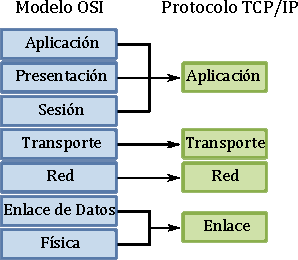
\includegraphics[scale=0.9]{Imagenes/MarcoTeorico/ModeloOSI-TCP-IP.pdf}
	\end{center}
	\caption{Modelo OSI relacionado con el modelo TCP/IP.} \label{fig:cap2:PC:TCPIP1}
\end{figure}

\subsubsection{Capa de enlace}

La capa de enlace o capa de interfaz de red es responsable de gestionar el medio f�sico, tal como LAN (Etnernet) o WAN. Todos los equipos conectados a Internet implementan este nivel \cite{Cap2Bib:Cisco, Cap2Bib:NetworkProtocols, Cap2Bib:IndustrialCT}.

Algunos ejemplos relevantes de protocolos en esta capa son los siguientes: ARP (\emph{Address Resolution Protocol}), HDLC (\emph{High-level Data Link Dontrol}) y PPP (\emph{Point-to-Point Protocol}).

\subsubsection{Capa de internet}

La capa de Internet es responsable de la comunicaci�n m�quina a m�quina, en donde una m�quina puede ser un anfitri�n\footnote{Computadora} (\emph{host}) o una puerta de enlace (\emph{gateway}) \cite{Cap2Bib:Cisco, Cap2Bib:NetworkProtocols, Cap2Bib:IndustrialCT}.

El paquete (de informaci�n) recibido de la capa de transporte, para su transmisi�n es encapsulado en un datagrama de Protocolo de Internet. La capa de Internet determina si enviar el datagrama directamente o a trav�s de una puerta de enlace, posteriormente env�a el datagrama a la capa de enlace para la transmisi�n.

La capa de Internet tambi�n se encarga de los datagramas de entrada. Se verifica la validez de cada datagrama y se determina si el datagrama deber�a ser procesado de manera local o ser enviado.

Algunos protocolos de la capa de Internet son: IP e ICMP (\emph{Internet Control Message Protocol}).

\subsubsection{Capa de transporte}

Esta capa tiene la responsabilidad de proveer la comunicaci�n entre las aplicaciones de \emph{software} del \emph{host} fuente y el \emph{host} destino y regular el flujo de informaci�n entre ellos \cite{Cap2Bib:Cisco, Cap2Bib:NetworkProtocols, Cap2Bib:IndustrialCT}.

La capa de transporte tambi�n provee mecanismos confiables de transporte a la capa de aplicaci�n, asegur�ndose que los datos son pasados a la capa de aplicaci�n en la secuencia correcta, sin duplicidad y sin errores.

Algunos protocolos de la capa de transporte son: TCP y UDP (\emph{User Datagram Protocol}).

\subsubsection{Capa de aplicaci�n}

En este nivel los usuarios solicitan procesos de aplicaci�n que acceden a la red. La aplicaci�n interact�a con los protocolos de la capa de transporte para enviar o recibir los datos emitidos por los procesos \cite{Cap2Bib:Cisco, Cap2Bib:NetworkProtocols, Cap2Bib:IndustrialCT}.

Algunos de los protocolos comunes de la capa de aplicaci�n son: clientes y servidores de WWW, TELNET, FTP (\emph{File Transfer Protocol}) y SMTP (\emph{Simple Mail Transfer Protocol}).

\section{Herramientas de desarrollo de aplicaciones Web y de escritorio}

Los usuarios finales, de un sistema de monitoreo y control, requieren de GUIs para interactuar con los dispositivos de una planta industrial. Generalmente, dichas interfaces gr�ficas consisten en aplicaciones Web y de escritorio. 

Las aplicaciones Web son aplicaciones distribuidas que emplean la arquitectura Cliente/Servidor. Dicha arquitectura se caracteriza por tener los siguientes elementos \cite{Cap2Bib:PAInternet}: 

\begin{itemize}\itemsep=-0.5em
	\item Cliente: Es el que hace peticiones de servicio y normalmente son los que inician la comunicaci�n. 
	\item Servidores: Estos proveen servicios y esperan a recibir peticiones. Una vez que han recibido una petici�n, la resuelven y retornan una respuesta. 
\end{itemize}

Las aplicaciones Web se basan en el hecho de contar con toda la capacidad de procesamiento en un servidor Web que se accede desde un navegador Web. Las aplicaciones Web se desarrollan empleando numerosos lenguajes de programaci�n, entre ellos destacan: PHP, JavaScript y SQL.

Actualmente para el desarrollo de aplicaciones Web existen herramientas que facilitan su desarrollo y mantenimiento. Para PHP predominan los \emph{frameworks} con arquitectura Modelo Vista Controlador (MVC, \emph{Model View Controller}), �stos facilitan la creaci�n de aplicaciones Web gracias a que dividen el desarrollo en tareas sencillas e intuitivas para el desarrollador \cite{Cap2Bib:Yii2, Cap2Bib:Yii1}. Entre los frameworks m�s destacados se encuentran: Yii, Symfony, CodeIgniter, CakePHP y Zend.

Las interfaces de comunicaci�n entre dispositivos (RTU) y computadoras de un sistema SCADA, usualmente requieren de aplicaciones de escritorio, las cuales se desarrollan empleando lenguajes de programaci�n como: Java, C/C++ y Visual Basic.

En un sistema SCADA las aplicaciones Web y de escritorio requieren de bases de datos para almacenar informaci�n �til para el usuario. Existen programas denominados Sistemas Gestores de Bases de Datos (SGBD), que permiten almacenar y posteriormente acceder a los datos de forma r�pida y estructurada, los SGBDs m�s usados hoy en d�a son: MySQL, PostgreSQL, Oracle, Microsoft SQL Server, entre otros.

\subsection{Java}
Java es un lenguaje de programaci�n de prop�sito general, concurrente, basado en clases, orientado a objetos e independiente de la plataforma (Windows o Unix). Java fue desarrollado por Sun Microsystems en la d�cada de los 90s, gran parte de su sintaxis est� basada en los lenguajes de programaci�n C y C++, aunque su modelo de objetos es m�s simple y elimina las herramientas de bajo nivel \cite{Cap2Bib:Java}.

El concepto orientado a objetos se refiere a un m�todo de programaci�n y al dise�o del lenguaje. Es dise�ar el \emph{software} de forma que los distintos tipos de datos que usen est�n unidos a sus operaciones. Por lo tanto, los datos y el c�digo (funciones o m�todos) se combinan en entidades llamadas objetos. Un objeto puede verse como un paquete que contiene el comportamiento (c�digo) y el estado (datos).

\subsection{PHP}
PHP es un lenguaje interpretado por parte del servidor, dise�ado originalmente para la creaci�n de p�ginas Web din�micas, el cual se caracteriza por su potencia, versatilidad, robustez y modularidad \cite{Cap2Bib:Yii2, Cap2Bib:Yii1}.
 
Los programas escritos en PHP son embebidos directamente en el c�digo HTML y ejecutados por el servidor Web a trav�s de un int�rprete antes de transferir al cliente, que lo ha solicitado, un resultado en forma de c�digo HTML puro. 

PHP es un lenguaje multiplataforma (Windows y Unix). En la actualidad PHP permite realizar una multitud de tareas en el entorno Web, por ejemplo: sistemas de correo electr�nico v�a Web, funciones de gesti�n y administraci�n de bases de datos, funciones de gesti�n de directorios y ficheros, funciones de tratamiento de im�genes y librer�as de funciones gr�ficas y funciones para la generaci�n de documentos en formato pdf.

\subsection{MySQL}

MySQL es un sistema gestor de bases de datos (SGBD o DBMS, \emph{Data Base Managment System}) r�pido, robusto y f�cil de usar. Permite la administraci�n de datos en un entorno de red, especialmente en las arquitecturas Cliente/Servidor. Cuenta con muchas herramientas y es compatible con varios lenguajes de programaci�n (por ejemplo PHP y Java), tambi�n es compatible con el servidor de p�ginas Web Apache \cite{Cap2Bib:MySQL}.

Las principales caracter�sticas de MySQL son las siguientes: 
\begin{itemize}\itemsep=-0.5em
\item Est� escrito en C/C++ y probado en numerosos compiladores. 
\item Funciona en sistemas operativos Windows y Unix. 
\item Dispone de un driver ODBC (\emph{Open DataBase Conectivity}) para Windows, aportando compatibilidad con la mayor�a de lenguajes de programaci�n de este sistema operativo. 
\item Se puede comunicar haciendo uso del lenguaje SQL, lo cual permite que sea compatible con otros sistemas de administraci�n de bases de datos.
\end{itemize}

\subsection{Framework Yii}

Yii es un \emph{framework} de aplicaciones Web escrito en PHP5, de alto rendimiento y basado en componentes. El nombre Yii es un acr�nimo de \emph{Yes, it is}. Yii abarca la filosof�a de convenci�n sobre configuraci�n, es decir, que tiene par�metros por defecto para casi todos los aspectos usados en la configuraci�n de una aplicaci�n. Gracias a esto, se requiere escribir menos c�digo y toma menos tiempo para desarrollar una aplicaci�n. Sin embargo, permite personalizar todos los par�metros por defecto para un uso en particular \cite{Cap2Bib:Yii2, Cap2Bib:Yii1}.

Yii puede ser usado en aplicaciones a cualquier escala, lo que significa que se puede desarrollar una aplicaci�n sencilla (relativamente) como un sitio Web informativo, como una aplicaci�n de uso empresarial o industrial. Yii fomenta la reusabilidad de c�digo en la mayor medida posible en la programaci�n Web, lo que acelera significativamente el proceso de desarrollo.

El \emph{framework} Yii est� dise�ado para ayudar a desarrollar con la filosof�a DRY (\emph{Don't Repeat Yourself}), el cual es un concepto clave en el desarrollo de aplicaciones �giles. Todas las aplicaciones Yii son construidas usando la arquitectura MVC, por ello, este patr�n de desarrollo se fomenta con la asignaci�n de directorios (Rutas) espec�ficos en donde se almacena cada fragmento de c�digo MVC. Esto minimiza la duplicaci�n de c�digo, promueve la reusabilidad de c�digo y facilita el mantenimiento. En la figura~\ref{fig:cap2:YiiMVC} se ilustra el diagrama de la estructura est�tica de una aplicaci�n Yii.

\begin{figure}[htb]
	\begin{center}
		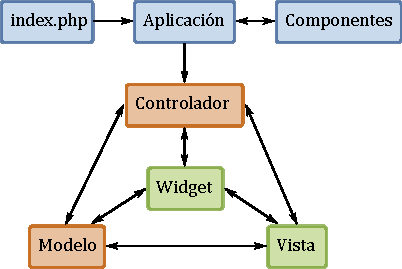
\includegraphics[scale=0.9]{Imagenes/MarcoTeorico/YiiMVC.pdf}
	\end{center}
	\caption{Arquitectura MVC del framework Yii.} \label{fig:cap2:YiiMVC}
\end{figure}

Los componentes de la arquitectura MVC se describen a continuaci�n:
\begin{itemize}\itemsep=-0.5em
\item \emph{Modelo}: En una arquitectura MVC, el Modelo es responsable de la informaci�n y debe encapsular las reglas de intercambio (\emph{Business Rules}) que aplican a dicha informaci�n.
En Yii se hace uso del patr�n de dise�o \emph{Active Record} (AR) para el acceso de base de datos abstracto en forma de objetos. Es decir, se obtienen las relaciones (Tablas) de la base de datos en forma de objetos PHP.
\item \emph{Vista}: La Vista es responsable de presentar la interfaz de usuario, la cual frecuentemente est� basada en la informaci�n contenida en los modelos. En la Vista se puede hacer uso de \emph{Widgets}, que son peque�os programas o aplicaciones, usualmente presentados en archivos o ficheros peque�os que son ejecutados por un motor de widgets o \emph{Widget Engine}. Actualmente existen muchos widgets para el framework Yii y son utilizados para acelerar el desarrollo.

\item \emph{Controlador}: El Controlador es el actor y director principal de una solicitud a una ruta (de la aplicaci�n). Es responsable de tomar los datos de entrada del usuario (que realiz� la solicitud), interactuar con el Modelo e indicar a la Vista que se actualice y despliegue apropiadamente la informaci�n solicitada.
\end{itemize}

En la figura~\ref{fig:cap2:YiiRequest} y~\ref{fig:cap2:YiiRequestSimplified} se ilustra, de manera detallada y simplificada respectivamente, el flujo de trabajo en una aplicaci�n Yii cuando se procesa una solicitud realizada por el usuario final \cite{Cap2Bib:Yii2, Cap2Bib:Yii1}.

\begin{figure}[htb]
	\begin{center}
		\begin{tabular}{c}
			\subfloat[Flujo detallado.]{%
				\label{fig:cap2:YiiRequest}%
				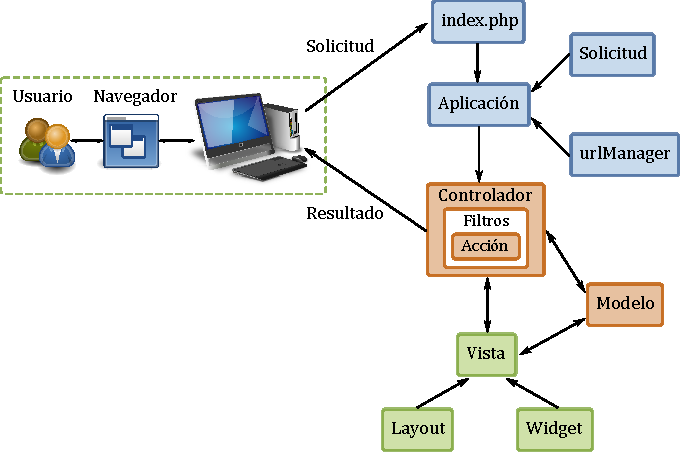
\includegraphics[scale=0.9]{Imagenes/MarcoTeorico/YiiRequest.pdf}}\\
			\subfloat[Flujo simplificado]{%
				\label{fig:cap2:YiiRequestSimplified}%
				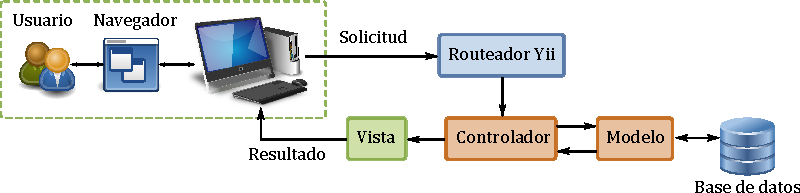
\includegraphics[scale=0.9]{Imagenes/MarcoTeorico/YiiRequestSimplified.pdf}} \\
		\end{tabular}	
	\end{center}
	\caption{Flujo de trabajo en una aplicaci�n Yii.} \label{fig:cap2:YiiApp}
\end{figure}

Los diagramas de flujo de trabajo de la figura~\ref{fig:cap2:YiiApp} se describen paso a paso de la siguiente manera:
\begin{itemize}\itemsep=-0.5em

\item El usuario realiza una solicitud a trav�s de una URL y el servidor Web la procesa ejecutando el \emph{script} (archivo de c�digo) principal index.php. El cual crea una instancia de la Aplicaci�n y la ejecuta.
\item La aplicaci�n obtiene informaci�n detallada de la solicitud del usuario.
\item La aplicaci�n determina el controlador y acci�n con la ayuda del componente de la aplicaci�n llamado urlManager y crea una instancia de dicho controlador para procesar la solicitud del usuario.
\item Al realizar una Acci�n principalmente se tienen dos casos: que el usuario desee guardar o modificar informaci�n de un Modelo o simplemente pedir informaci�n del mismo.
\item La Acci�n despliega una vista con la informaci�n del Modelo. Generalmente las vistas est�n asociadas a las Acciones de un Controlador.
\item La vista puede ejecutar widgets y el resultado de la presentaci�n es empotrada (Integrada) en el dise�o principal (\emph{Layout}).
\item Por �ltimo, la acci�n completa la presentaci�n de la vista desplegando el resultado al usuario.
\end{itemize}

\subsection{JavaScript}

JavaScript es un lenguaje de programaci�n para el desarrollo de aplicaciones con arquitectura Cliente/Servidor a trav�s de Internet. Una aplicaci�n en JavaScript tiene la particularidad de que est� insertado dentro del mismo documento HTML, el cual presenta dicha aplicaci�n al usuario \cite{Cap2Bib:Javascript}. 

Una aplicaci�n en JavaScript, es un sistema interactivo que tiene la capacidad de detectar eventos o acciones realizadas por los usuarios. JavaScript fue dise�ado para ser un lenguaje de elaboraci�n de \emph{scripts} que pudieran incrustarse en archivos HTML. No es compilado, sino que, en vez de ello, es interpretado por el navegador como c�digo fuente.

En la actualidad existen muchas herramientas que aceleran el desarrollo de aplicaciones usando JavaScript, estas herramientas se denominan frameworks. Los framework de JavaScript m�s populares son: JQuery, Ext JS, Prototype, entre otros.



% Variable local para emacs, para que encuentre el fichero maestro de
% compilaci�n y funcionen mejor algunas teclas r�pidas de AucTeX
%%%
%%% Local Variables:
%%% mode: latex
%%% TeX-master: "../Tesis.tex"
%%% End:

		%------------------------
%Cap�tulo 3: Desarrollo
%------------------------

\chapter{Desarrollo del sistema}
\label{cap3}

En este cap�tulo se presenta el desarrollo del prototipo de sistema de monitoreo para la PTAR de la UTM utilizando una metodolog�a de desarrollo para mejoramiento de procesos de producci�n. Dicha metodolog�a es conocida como Modelo de Integraci�n de Capacidad y Madurez (CMMI, \emph{Capability Maturity Model Integration}) \cite{Cap2Bib:CMMI}.

CMMI consiste de 5 niveles de madurez y cada nivel consta de un n�mero de �reas de procesos. Sin embargo, debido a que en los diferentes niveles del modelo CMMI existen �reas de procesos enfocadas a organizaciones o empresas ya establecidas, la aplicaci�n de CMMI en el desarrollo de este sistema se limit� a aspectos de ingenier�a, por lo que solo se implementaron los niveles 1, 2 y 3. Estos niveles de detallan en la figura~\ref{fig:cap3:CMMI}.

\begin{figure}[htb]
	\begin{center}
		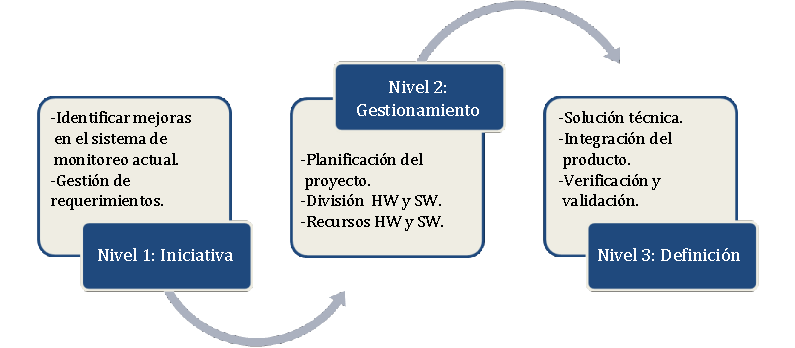
\includegraphics[scale=0.9]{Imagenes/Desarrollo/CMMI.pdf}
	\end{center}
\caption{Niveles de la metodolog�a CMMI.} \label{fig:cap3:CMMI}
\end{figure}

\section{Iniciativa}

\subsection{Estado actual de la PTAR}

En la PTAR de la UTM no se cuenta con un sistema automatizado para el monitoreo de pH y OD, por lo que este proceso se realiza manualmente. 

El monitoreo de pH se realiza mediante los siguientes pasos:
\begin{enumerate} \itemsep=-0.7em
\item Se toma una muestra de 50ml de agua residual. 
\item Con un potenci�metro se toma la lectura del pH. 
\item Se registra el valor de la medici�n en una bit�cora.
\item Se tabulan los resultados.
\end{enumerate}

El monitoreo de ox�geno disuelto (OD) se realiza de la siguiente manera:

\begin{enumerate} \itemsep=-0.7em
\item Se calibra previamente el electrodo de $O_2$, el cual se utiliza para medir este par�metro.
\item Se sumerge el electrodo en el bioreactor y se toman las lecturas.
\item Se registra el valor de la medici�n en una bit�cora. 
\item Se tabulan los resultados.
\end{enumerate}


Por lo anterior y considerando que no se lleva a cabo el monitoreo de temperatura, se propone realizar la medici�n de pH, OD y temperatura mediante un sistema automatizado, almacenar registros de las mediciones en una base de datos y mostrar gr�ficamente y de manera tabular el historial de los registros de mediciones.

\subsection{Propuesta}

El sistema que se propone desarrollar tiene como objetivo implementar un sistema SCADA para monitorear remotamente y de manera automatizada el estado de pH, OD y temperatura de la PTAR de la UTM. Dicho sistema consta de sensores de prop�sito industrial, los cuales se describen en la secci�n~\ref{cap2:sec:Sensores}; una RTU; la MTU; un sistema de comunicaciones que consta de una interfaz serie RS-485; servidores de procesamiento distribuido; y, acceso Web con una interfaz de usuario. En la figura~\ref{fig:cap3:DBscada} se muestra un diagrama general del sistema propuesto.

\begin{figure}[htb]
	\begin{center}
 		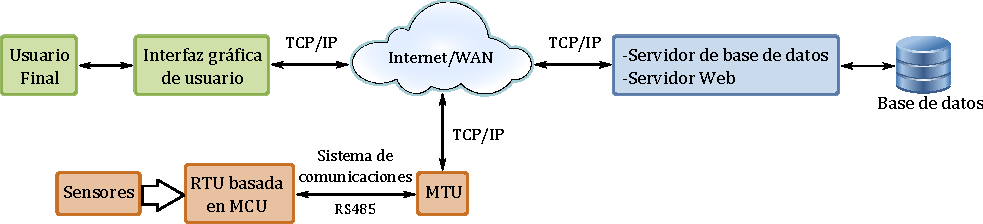
\includegraphics[scale=0.9]{Imagenes/Desarrollo/DBScada.pdf}
	\end{center}
	 \caption{Diagrama general del sistema SCADA.} \label{fig:cap3:DBscada}
\end{figure}

El sistema realizar� el monitoreo de manera automatizada, las mediciones ser�n tomadas discretamente, es decir, se tomar�n mediciones cada cierto intervalo de tiempo. El sistema almacenar� registros de mediciones en una base de datos y mediante una aplicaci�n Web proporcionar� una interfaz de usuario. El usuario del sistema podr� visualizar el estado de pH, OD y temperatura de la PTAR desde cualquier lugar a trav�s de una computadora (Cliente) con acceso a Internet.

\section{Gestionamiento}

\subsection{Requerimientos funcionales de la propuesta}

En la figura~\ref{fig:cap3:DB2scada} se muestra de manera detallada el sistema SCADA propuesto. Este sistema realizar� el monitoreo remoto de pH, OD y temperatura de la PTAR. Las mediciones proporcionadas por cada sensor pasar�n por una etapa de acondicionamiento de se�al mediante un sistema electr�nico (CAS,\emph{Circuito de Acondicionamiento de Se�al}). El MCU ATmega8 desempe�ar� el papel de RTU, implementar� las funciones del protocolo Modbus, procesar� solicitudes de la MTU y realizar� la adquisici�n de datos de los sensores a trav�s de un m�dulo ADC (integrado en el MCU). El sistema de comunicaciones implementar� una interfaz serie RS-232/RS-485 a trav�s de un transceptor (\emph{Transceiver}), que servir� para la comunicaci�n entre la RTU y la MTU. La MTU (Computadora) implementar� las funciones del protocolo Modbus para solicitar informaci�n de la RTU, almacenar� registros de mediciones en una base de datos y recibir� �rdenes que emite el usuario a trav�s de la interfaz Web. Los servidores proporcionan el gestor de bases de datos, la base de datos y la aplicaci�n Web (Interfaz gr�fica del usuario final). La aplicaci�n Web incluye, la gesti�n de usuarios (Administrador), visualizaci�n de tendencias y de entradas y salidas digitales.

\begin{figure}[htb]
	\begin{center}
 		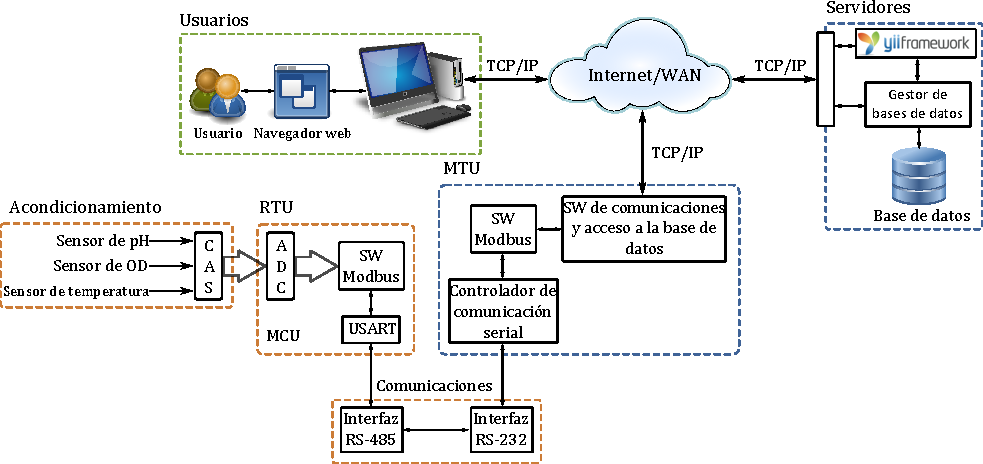
\includegraphics[scale=0.9]{Imagenes/Desarrollo/DBScada2.pdf}
	\end{center}
	 \caption{Diagrama completo del sistema SCADA propuesto.} \label{fig:cap3:DB2scada}
\end{figure}

\subsubsection{Clasificaci�n y an�lisis de requerimientos}

Los requerimientos funcionales de la propuesta, para un mejor an�lisis, son clasificados de la siguiente manera:

\begin{itemize} \itemsep=-0.5em
	\item \emph{Acondicionamiento de se�al}: La se�al que proviene de los sensores requiere de una etapa de acondicionamiento, por ello se hace uso de un sistema de acondicionamiento de se�al o CAS. El CAS emplea un sistema electr�nico, el cual tiene como entrada la se�al de un sensor y proporciona en la salida un nivel de se�al o voltaje adecuado para el funcionamiento de la etapa posterior de adquisici�n de datos. 
	\item \emph{Especificaci�n del CAS de cada sensor}: Para los sensores de pH y temperatura, el CAS para cada uno de ellos se ha dividido en tres etapas: Aislamiento, Filtrado y Amplificaci�n. El CAS para el sensor de OD se ha dividido en las siguientes etapas: Conversi�n de corriente a voltaje, Amplificaci�n y Filtrado. 
	\item \emph{Software de la RTU}: Para implementar la RTU del protocolo Modbus en el MCU ATmega8, se requiere de un \emph{software}. Dicho \emph{software} se construye en lenguaje C, en el que se codifican los par�metros de configuraci�n de perif�ricos de entrada/salida, los formatos de las ADU de solicitudes y respuestas y el procesamiento de solicitudes de la MTU.
	\item \emph{Funciones de la RTU}: Las funciones primordiales del MCU (RTU) son obtener mediciones de los sensores, proporcionar el voltaje de alimentaci�n para el sensor de OD, recibir y procesar las ADUs de solicitud que emite la MTU y construir y enviar las ADU de respuesta (con la informaci�n solicitada) a la MTU. 
	\item \emph{Comunicaci�n MTU-RTU}: La comunicaci�n entre la RTU y la MTU se realizar� a trav�s de una interfaz serie RS-485 como medio f�sico. La MTU (Computadora) cuenta con un puerto serie, cuyo funcionamiento se basa en el est�ndar RS-232, por ello, se requiere un transceptor entre las interfaces RS-485 y RS-232.
	\item \emph{Software de la MTU}: El protocolo Modbus de la MTU se implementar� desarrollando un \emph{software} en lenguaje Java, en el cual se codifican los formatos de las ADU de solicitudes y respuestas Modbus. 
	Este \emph{software} contar� con un controlador para la gestionar la comunicaci�n serie con la RTU (Figura~\ref{fig:cap3:RTUMTU2}), un gestor de monitoreo discreto de la RTU, un m�dulo que comunica la MTU con el servidor de bases de datos y un m�dulo de comunicaci�n con la aplicaci�n Web (Figura~\ref{fig:cap3:MTU-Servidores}).
	\item \emph{Servidor Web y base de datos}: La aplicaci�n Web se desarrollar� haciendo uso del Framework Yii (arquitectura MVC), dicha aplicaci�n restringir� el acceso s�lo al Administrador del sistema, permitir� (al Administrador) visualizar el estado de pH, OD y temperatura a trav�s de gr�ficas de tendencias, visualizar el estado de las alarmas a trav�s de indicadores (switch) y cambiar el estado de las salidas digitales en la RTU.
	\item \emph{Herramientas de dise�o y desarrollo}: En el dise�o\emph{hardware} se emplear�n herramientas de simulaci�n y dise�o de circuitos electr�nicos. Para el desarrollo del \emph{software} del MCU, se emplear� un entorno de desarrollo exclusivo del MCU, el cual utiliza el lenguaje de programaci�n C. En el desarrollo del \emph{software} de la MTU y de la aplicaci�n Web, se emplear�n entornos de desarrollo para lenguajes de programaci�n orientado a objetos y de alto nivel.
	\item \emph{Entradas y salidas digitales}: El MCU se configur� para incluir dos entradas y dos salidas digitales, aunque su implementaci�n con dispositivos externos no fue desarrollada, se permite conectar entradas y salidas digitales externas que est�n debidamente aisladas y que operen con niveles de voltaje TTL.
\end{itemize}

\begin{figure}[htb]
	\begin{center}
		\begin{tabular}{c}
			\subfloat[Comunicaci�n de la MTU con la RTU.]{%
				\label{fig:cap3:RTUMTU2}%
				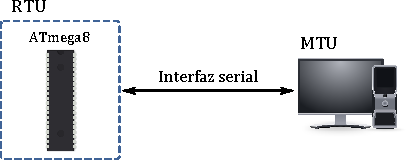
\includegraphics[scale=0.9]{Imagenes/Desarrollo/Dise�oSW/RTU-MTU2.pdf}} \\
			\subfloat[Comunicaci�n de la MTU con los Servidores.]{%
				\label{fig:cap3:MTU-Servidores}%
				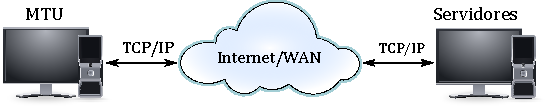
\includegraphics[scale=0.9]{Imagenes/Desarrollo/Dise�oSW/MTU-Servidores.pdf}} \\
		\end{tabular}
	\end{center}
	\caption{Comunicaci�n de la MTU con la RTU y con el servidor de la aplicaci�n Web y la base de datos.} \label{fig:cap3:MTU-RTU-Servidores}
\end{figure}

\subsection{Divisi�n \emph{hardware} y \emph{software}}

Las fases de dise�o e implementaci�n de \emph{hardware} y \emph{software} del sistema SCADA se realizaron utilizando la metodolog�a de desarrollo para Sistemas Empotrados (\emph{Embedded Systems}) \cite{Cap2Bib:TesisDavid, Cap2Bib:EmbeddedSystems}. En base a los requerimientos del sistema, la divisi�n de tareas \emph{hardware} y \emph{software} se listan en la tabla~\ref{tab:cap3:Thwsw}.

\begin{table}[htp]
	\caption{Etapas \emph{hardware} y \emph{software}.}%
	\centering
	\footnotesize
	\begin{tabular}{ll}
		\hline \hline \hline \hline
		\rowcolor[gray]{0.8}\textbf{\emph{Hardware} }&\textbf{\emph{Software}}\\
		\hline \hline \hline \hline
		Acondicionamiento de los sensores & Dise�o \emph{software} de la RTU\\
		\rowcol Entradas y salidas de la RTU	& Dise�o \emph{software} de la MTU\\
		Interfaz RS-485	& Dise�o \emph{software} de la aplicaci�n Web\\
		\rowcol Transceptor RS-232/RS-485	\\
		\hline \hline \hline \hline
\end{tabular}
\label{tab:cap3:Thwsw}
\end{table}

\subsubsection{Selecci�n de hardware}
Los elementos \emph{hardware} seleccionados para satisfacer los requerimientos funcionales de la propuesta del sistema SCADA son:

\begin{itemize} \itemsep=-0.5em

	\item\emph{CA3140}: Es un \emph{op-amp} (\emph{Amplificador operacional}) con tecnolog�a MOSFET que cuenta con una alta impedancia de entrada ${Z}_{in}=1.5\tera\ohm$, opera con corrientes de entrada muy bajas ${I}_{min}=10\pico\ampere$ a un voltaje de alimentaci�n ${V}_{s}=\pm15\volt$. Su campo de aplicaci�n abarca las �reas de instrumentaci�n, filtros activos, generadores de funciones, instrumentos port�tiles, etc \cite{Cap2Bib:CA3140}.

	El op-amp CA3140 se utiliza para implementar todas las etapas del CAS (aislamiento, conversi�n corriente-voltaje, filtrado y amplificaci�n) de cada sensor.

	\item\emph{TL081}: Es un op-amp de bajo costo, de alta velocidad, con entrada JFET (\emph{Junction Field-Effect Transistor}) y con un voltaje offset de entrada internamente reducido. Este dispositivo requiere una baja corriente de alimentaci�n, sin embargo, ofrece un amplio ancho de banda de ganancia y r�pida velocidad de respuesta \cite{Cap2Bib:TL081}.
	
	EL CI TL081 puede ser usado en aplicaciones como integradores de alta velocidad, convertidores D-A (Digital An�logo), circuitos de muestreo y retenci�n y otras.
		
	\item\emph{Capacitor de poli�ster}: Sus principales aplicaciones son en sistemas de audio, equipos de instrumentaci�n y filtros. Por lo tanto, estos capacitores se utilizan en el dise�o de la etapa de filtrado del CAS de cada sensor.

	\item\emph{ATmega8}: Es un MCU de la marca ATMEL que cuenta con una arquitectura AVR RISC, memoria flash para c�digo de $8\kilo$B, frecuencia m�xima de operaci�n de $16\mega\hertz$, seis canales ADC, un dispositivo de comunicaci�n serie USART (\emph{Universal Synchronous and Asynchronous serie Receiver and Transmitter}), etc \cite{Cap2Bib:ATmega8}.

	El ATmega8 se utiliza para implementar la RTU, lo cual se logra codificando en la memoria de c�digo el protocolo Modbus y el \emph{software} de control, los canales ADC se utilizan para obtener las mediciones de los sensores, se asigna un puerto de salida de 8 bits que indica al DAC el nivel de voltaje para alimentar el sensor de OD y el dispositivo USART se utiliza para la comunicaci�n serie con la MTU.

	\item\emph{MAX489}: Es un circuito integrado (CI) de la marca MAXIM que tiene la funci�n de transceptor para comunicaciones RS-485, el cual permite una transmisi�n de datos libre de errores a una velocidad de $250\kilo$bps y se puede configurar para operar en modo\emph{full-duplex} y \emph{half-duplex} \cite{Cap2Bib:MAX489}.

	El CI MAX489 se utiliza para implementar la interfaz RS-485, lo cual se logra al conectarse con el dispositivo USART del ATmega8.

	\item\emph{MAX232}: Es un CI de la marca MAXIM que convierte las se�ales de un puerto serie RS-232 a se�ales compatibles con niveles TTL \cite{Cap2Bib:MAX232}.

	El CI MAX232 se utiliza para la comunicaci�n serie entre la MTU y la RTU, debido a que el puerto serie de la MTU (computadora) basa su funcionamiento de acuerdo al est�ndar RS-232.

	\item\emph{DAC0808}: Es un DAC de 8 bits con un tiempo de establecimiento a escala completa de $150\milli\second$, cuenta con un registro de entrada de 8 bits que indica el nivel de voltaje a generar y opera con fuentes de alimentaci�n de $\pm5\volt$ \cite{Cap2Bib:DAC0808}.

	El CI DAC0808 se utiliza para generar el voltaje de alimentaci�n del sensor de OD, por lo que el registro de entrada se conecta al registro de proporciona el ATmega8.
\end{itemize}

En la tabla~\ref{tab:cap3:tareas-componentes-hw} se muestra la relaci�n entre las tareas HW y los elementos HW seleccionados.

\begin{table}[htb]
	\caption{Relaci�n entre tareas y componentes hardware.}%
	\centering
	\footnotesize
	\begin{tabular}{p{2in}cccccc}
		\hline \hline \hline \hline
		\rowcolor[gray]{0.8} \textbf{Tareas hardware}&\textbf{CA3140}&\textbf{Capacitor}&\textbf{ATmega8}&\textbf{MAX232}&\textbf{MAX489}&\textbf{DAC0808}\\
		\hline \hline \hline \hline
		Acondicionamiento &	X	&	X	&	&	&	&\\
		\rowcol Entradas/salidas de la RTU	&	&	&	X	&	&	&	\\
		Interfaz RS-232/RS-485	&	&	&	X	&	X	&	X	&\\
		\rowcol Alimentaci�n del sensor de OD	&	&	&	X	&	&	&	X\\
		\hline \hline \hline \hline
	\end{tabular}
	\label{tab:cap3:tareas-componentes-hw}
\end{table}

\subsubsection{Selecci�n de herramientas \emph{software} de dise�o y desarrollo}

Las herramientas de dise�o de \emph{hardware} y \emph{software} seleccionados para el desarrollo de la propuesta se describen a continuaci�n:

\begin{itemize} \itemsep=-0.5em

\item\emph{AVR Studio}: Herramienta \emph{software} de la compa��a ATMEL versi�n 4.16 proporcionada de forma gratuita. Es un entorno de desarrollo de aplicaciones para MCUs del mismo fabricante, el cual permite escribir, compilar y depurar c�digos en lenguaje C/C++ y lenguaje ensamblador.

\item\emph{Proteus	Design Suite}: Herramienta \emph{software} en la versi�n 7.6, la cual es desarrollada y comercializada por \emph{Labcenter Electronics Ltd}. Permite el dise�o de diagramas esquem�ticos, simulaci�n de circuitos mediante un sistema basado en SPICE e incluye una suite de herramientas de dise�o de PCB.

\item\emph{Cadence OrCAD}: Es una herramienta \emph{software} comercial de \emph{Cadence Design Systems, Inc}. en su versi�n 10.3 permite dise�ar y editar diagramas esquem�ticos para el desarrollo de PCB o simulaci�n anal�gica utilizando modelado SPICE.

\item\emph{Docklight}: Es un producto \emph{software} de \emph{Flachmann \& Heggelbacher}, en la versi�n 1.9.21, ayuda a realizar pruebas de conexi�n y comunicaci�n en interfaces serie. 

\item\emph{Netbeans}: Herramienta de \emph{software} libre (\emph{Open Source}) desarrollada y mantenida por la comunidad \emph{Netbeans} (\emph{NetBeans Community}). Se utilizaron las versiones 7.0.1 y 7.3.1, esta herramienta es un entorno de desarrollo integrado (IDE, \emph{Integrated Development Environment}) que permite el desarrollo de aplicaciones escritas en lenguaje \emph{Java}, \emph{JavaScript}, \emph{PHP} y otros. Tambi�n provee un m�dulo para el dise�o de GUIs en Java.

\item\emph{Eclipse}: Herramienta de \emph{software} libre desarrollada y soportada por la comunidad \emph{Eclipse}, en la que personas y organizaciones colaboran para desarrollar y mejorar dicha herramienta. Se utiliz� la versi�n 3.7, el cual es un IDE para el desarrollo de aplicaciones escritas en lenguaje C/C++, Python, Java, JavaScript, PHP y otros. Eclipse proporciona herramientas para el desarrollo de GUIs.

\item\emph{PHPEdit}: Herramienta \emph{software} propiedad de \emph{WaterProof SARL}. Se utiliz� la versi�n 4.2, esta herramienta es un IDE para desarrollo PHP que permite crear sitios web din�micos, codificar y depurar PHP, y realizar pruebas de proyecto.

\item \emph{Enterprise Architect}: Es un producto propiedad de \emph{SPARX SYSTEMS}. En la versi�n 9 de evaluaci�n, es un conjunto de herramientas para modelado y dise�o de \emph{software}, por lo que sirve de asistente en la gesti�n de proyectos \emph{software}, proporcionando m�ltiples herramientas de modelado y herramientas de creaci�n de diagramas que facilitan el desarrollo.

\item\emph{XAMPP}: Las herramientas necesarias para el desarrollo de la aplicaci�n Web, est�n contenidas en la suite XAMPP en la versi�n 1.8.1. Esta suite contiene las siguientes herramientas: PHP 5.4.7 (requerido para desarrollar la aplicaci�n Yii), gestor de base de datos MySQL 5.5.27, servidor Apache 2.4.3 y otros.

\item\emph{Framework Yii}: Para desarrollar la aplicaci�n Web se utiliz� el \emph{Framework Yii versi�n 1.1.13}. Yii, por ser un Framework de \emph{software} libre, est� en constante evoluci�n, por lo que actualmente hay nuevas versiones que incluyen algunas mejoras.

\end{itemize}

\section{Definici�n}

\subsection{Dise�o hardware}
\label{cap3:Definicion:DHW}
Como se describe en la tabla~\ref{tab:cap3:Thwsw}, el desarrollo del sistema se divide en cuatro etapas \emph{hardware}. Estas etapas se describen a continuaci�n: 

\begin{itemize} \itemsep=-0.5em
	\item \emph{Etapa de acondicionamiento de los sensores}: En esta etapa se detalla el dise�o espec�fico de acondicionamiento para cada sensor en particular.
	\item\emph{Entradas y salidas de la RTU}: Esta etapa describe la configuraci�n de entradas y salidas del MCU ATmega8 y la distribuci�n de terminales.
	\item\emph{Interfaz RS-485}: Describe la configuraci�n de la interfaz serie RS-485.
	\item\emph{Transceptor RS-232/RS-485}: Especifica el dise�o de la comunicaci�n entre las interfaces RS-485 y RS-232. La interfaz RS-485 es usada por la RTU y la interfaz RS-232 es usada por la MTU.
\end{itemize}

\subsubsection{Dise�o de la etapa de acondicionamiento de los sensores}

\paragraph{CAS del sensor de pH}
\label{Cap3:DHWCASpH}
El dise�o del CAS para el sensor de pH consiste de tres etapas, como se ilustra en la figura~\ref{fig:cap3:CAS1}, las cuales son: aislamiento, filtrado y amplificaci�n. No obstante, como se describe en la subsecci�n~\ref{cap2:Sensores:pH}, se indica que el voltaje de la se�al de salida del sensor de pH (${V}_{pH}$) oscila entre $-414.12\milli\volt$ y $+414.12\milli\volt$, por lo cual, se requiere de una etapa previa en la que se agrega un voltaje de desplazamiento (\emph{offset}), el cual deber� ser mayor a $414\milli\volt$. Con ello se garantiza una se�al de salida con voltaje positivo, que es aceptable para la entrada del ADC, ya que el ADC solo acepta niveles de voltaje positivos.

\begin{figure}[htb]
	\begin{center}
		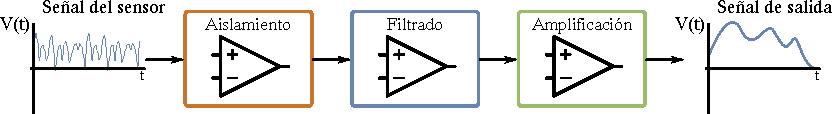
\includegraphics[scale=0.9]{Imagenes/Desarrollo/Dise�oHardware/CAS1.pdf}
	\end{center}
	 \caption{Etapas del CAS para el sensor de pH y de temperatura.} \label{fig:cap3:CAS1}
\end{figure}

Para la etapa que genera el voltaje \emph{offset} (${V}_{offset}$) se emplea el regulador de voltaje LM317 con la configuraci�n de limitador de corriente y el op-amp TL081 como seguidor de voltaje (Figura~\ref{fig:cap3:offph}) \cite{Cap2Bib:Alexander, Cap2Bib:Coughlin, Cap2Bib:Hayt}. 

La idea de construir una fuente de voltaje fija para generar ${V}_{offset}$ empleando el CI LM317, surgi� de~\cite{Cap2Bib:Voffset}, en donde se muestra que es posible obtener una fuente de corriente constante a partir de dicho dispositivo y al variar la resistencia de carga se ajusta el voltaje de salida. En base a los c�lculos propuestos en~\cite{Cap2Bib:Voffset} se obtuvo la siguiente configuraci�n (Figura~\ref{fig:cap3:SimVoffset}): $R_1 = 10\kilo\ohm$ y $R_2 = 3.2\kilo\ohm$ para obtener ${V}_{offset} = 400\milli\volt$. Sin embargo, en la simulaci�n que se muestra en la figura~\ref{fig:cap3:SimVoffset}, se obtuvo ${V}_{offset} = 577\milli\volt$. 

No obstante, debido a que las especificaciones del LM317 var�an con cada fabricante, este dise�o no funcion� de la misma manera en la pr�ctica. Por lo que en la figura figura~\ref{fig:cap3:offph} se muestra la configuraci�n funcional del LM317 en donde se obtiene ${V}_{offset} = 505.6\milli\volt$ como se detalla en la secci�n~\ref{cap04:VOffset}. Con lo que se garantiza un desplazamiento de la se�al ${V}_{pH}$ para obtener niveles de voltaje positivo.

La etapa de aislamiento es requerida debido a la alta impedancia de salida del sensor de pH. En dicha etapa se utiliza el CI CA3140 configurado como seguidor de voltaje (figura~\ref{fig:cap3:offph}) con lo que se obtiene ${V}_{ApH}={V}_{pH}+{V}_{offset}$.

\begin{figure}[htb]
	\begin{center}
		\begin{tabular}{c}
			\subfloat[Adici�n de ${V}_{offset}$ y aislamiento del sensor de pH.]{%
				\label{fig:cap3:offph}%
				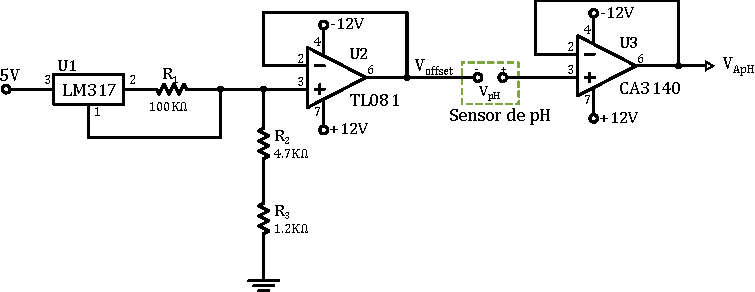
\includegraphics[scale=0.9]{Imagenes/Desarrollo/Dise�oHardware/CASpHOffset.pdf}} \\
			\subfloat[Simulaci�n de la etapa de adici�n de ${V}_{offset}$.]{%
				\label{fig:cap3:SimVoffset}%
				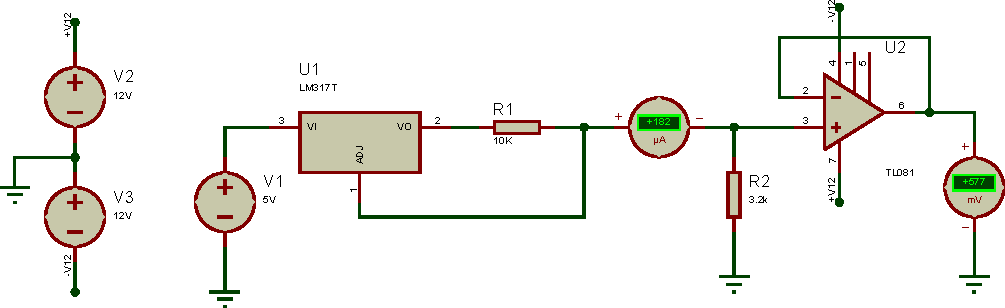
\includegraphics[scale=0.85]{Imagenes/Desarrollo/Dise�oHardware/SimulacionVoffset.pdf}} \\
		\end{tabular}	
	\end{center}
	\caption{Configuraci�n y simulaci�n de la etapa de adici�n de ${V}_{offset}$ y etapa de aislamiento para el CAS de pH.} \label{fig:cap3:Voffset_pH}
\end{figure}

En la etapa de filtrado se emplea la configuraci�n de un filtro activo pasa-bajas, como el de la figura~\ref{fig:cap3:filph} \cite{Cap2Bib:Alexander, Cap2Bib:Coughlin, Cap2Bib:Hayt}, en donde el filtrado se realiza utilizando un circuito \emph{RC} y el CI \emph{CA3140} como amplificador de ganancia variable, con ello la amplificaci�n se incluye en el dise�o de la misma etapa de filtrado\footnote{La configuraci�n completa del CAS del sensor de pH se muestra en el ap�ndice~\ref{ap:HWSch}.}.

\begin{figure}[htb]
	\begin{center}
		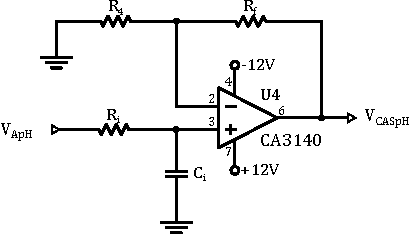
\includegraphics[scale=0.9]{Imagenes/Desarrollo/Dise�oHardware/CASpH.pdf}
	\end{center}
	\caption{Configuraci�n del filtro \emph{pasa-bajas} con ganancia ajustable.} \label{fig:cap3:filph}
\end{figure}

La frecuencia de corte ${f}_{c}$ del filtro \emph{pasa-bajas} se calcula con la ecuaci�n~\ref{cap3:eq:pHfc} y la ganancia de amplificaci�n ${G}_{a}$ se calcula con la ecuaci�n~\ref{cap3:eq:pHG}.

\begin{equation} \label{cap3:eq:pHfc}
{w}_{c}={{1}\over{{R}_{i}{C}_{i}}}=2\pi{f}_{c}
\end{equation}

\begin{equation} \label{cap3:eq:pHG}
{G}_{a}=(1+{{R}_{f}\over{R}_{4}})
\end{equation}

en estas ecuaciones se tiene que: 

\begin{variables}
	\item[${w}_{c}=$] Frecuencia de corte en [$\rad\per\second$].
	\item[${f}_{c}=$] Frecuencia de corte en [$\hertz$].
	\item[${R}_{i}=$] Resistencia del circuito RC.
	\item[${C}_{i}=$] Capacitor del circuito RC.
	\item[${G}_{a}=$] Ganancia del amplificador.
	\item[${R}_{f}=$] Resistencia de retroalimentaci�n del amplificador.
	\item[${R}_{4}=$] Resistencia de entrada del amplificador.
\end{variables}

Debido a que la se�al del sensor de pH es propensa a contaminarse con ruido, se establece una frecuencia de corte baja ${f}_{c}=0.159\hertz$. Para una mejor compatibilidad con el ADC del ATmega8, se eligi� una ganancia de amplificaci�n ${G}_{a}=2$. Los par�metros para el c�lculo del filtro y el amplificador se muestran en la tabla~\ref{tab:cap3:CASpH}.

\begin{table}[htb]
	\caption{Par�metros usados en el CAS del sensor de pH.}%
	\centering
	\footnotesize
	\begin{tabular}{ccc}
		\hline \hline \hline \hline
		\rowcolor[gray]{0.8}\textbf{Par�metro}&\textbf{Valor}&\textbf{Unidad}\\
		\hline \hline \hline \hline
		
		${R}_{i}$&$10$&$\mega\ohm$\\
		\rowcol ${C}_{i}$&$100$&$\nano\farad$\\
		${f}_{c}$&$0.159$&$\hertz$\\
		\rowcol ${R}_{f}$&$470$&$\kilo\ohm$\\
		${R}_{1}$&$470$&$\kilo\ohm$\\
		\rowcol ${G}_{a}$&$2$&-\\
		\hline \hline \hline \hline
	\end{tabular}
	\label{tab:cap3:CASpH}
\end{table}

Por todo lo anterior, el modelo matem�tico del dispositivo CAS para el sensor de pH se describe en la siguiente ecuaci�n:

\begin{equation} \label{cap3:eq:VCASpH}
{V}_{CASpH} = 2({V}_{pH}+{V}_{offset})
\end{equation}

En la figura~\ref{fig:cap3:SimulacionVCASpH} se muestra la simulaci�n completa del CAS del sensor de pH. En la simulaci�n se sustituye la entrada del sensor de pH por una fuente de voltaje (${V}_{pH}$). Se considera que el dominio (entrada del CAS) est� en el rango de voltaje de $-414.12\milli\volt$ a $+414.12\milli\volt$, con ello, en la figura~\ref{fig:cap4:SimCASpH} y en la tabla~\ref{tab:cap4:SimulacionCASpH1} se muestran los resultados que arroja la simulaci�n de manera gr�fica y tabular respectivamente.

\begin{figure}[htb]
	\begin{center}
		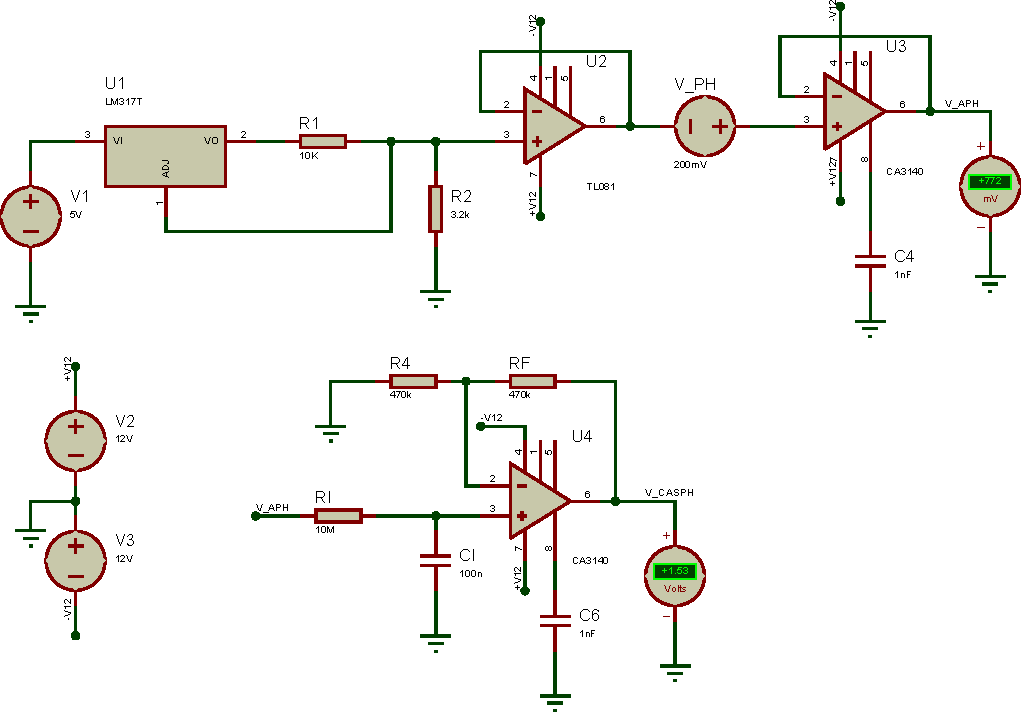
\includegraphics[scale=0.85]{Imagenes/Desarrollo/Dise�oHardware/SimulacionVCASpH.pdf}
	\end{center}
	\caption{Simulaci�n Completa del CAS para el sensor de pH.} \label{fig:cap3:SimulacionVCASpH}
\end{figure}

\begin{center}
	\pgfplotsset{every axis/.append style={thick,tick style={thin},font=\footnotesize}}
\begin{tikzpicture}
\tikzset{
every pin/.style={fill=yellow!50!white,rectangle,rounded corners=3pt,font=\scriptsize},
small dot/.style={fill=black,circle,scale=0.3}
}
	\begin{axis}[use units,x=5cm,y=2cm,
		minor tick num=3,
		axis y line=middle,
		axis x line=middle,
		x unit=V,xlabel=${V}_{pH}$,
		y unit=V,ylabel=${V}_{CASpH}$,
		ymin=0
				]
		\addplot[smooth,blue, domain=-3:3] table[x={vph}, y={vcasph}]{CASpHSimulation.data};
	\end{axis}
\end{tikzpicture}



	\captionof{figure}{Gr�fica de entradas y salidas de la simulaci�n del CAS para el sensor de pH.} \label{fig:cap4:SimCASpH}
\end{center}

\begin{table}[htp]
	\caption{Tabla de entradas y salidas de la simulaci�n del CAS para el sensor de pH.}%
	\centering
	\footnotesize
	\begin{tabular}{cc}
		\hline \hline \hline \hline
		\headcol$\pmb{{V}_{pH}}$&$\pmb{{V}_{CASpH}}$\\
		\hline \hline \hline \hline
		$400\milli\volt$ & $1.93\volt$\\
		\rowcol $300\milli\volt$ & $1.73\volt$\\
		$200\milli\volt$ & $1.53\volt$\\
		\rowcol $100\milli\volt$ & $1.33\volt$\\
		$0\volt$ & $1.13\volt$\\
		\rowcol $-100\milli\volt$ & $934\milli\volt$\\
		$-200\milli\volt$ & $734\milli\volt$\\
		\rowcol $-300\milli\volt$ & $534\milli\volt$\\
		$-400\milli\volt$ & $334\milli\volt$\\
		\hline \hline \hline \hline
	\end{tabular}
	\label{tab:cap4:SimulacionCASpH1}
\end{table} 

\paragraph{CAS del sensor de OD}

El dise�o del CAS para el sensor de OD se divide en dos etapas principales (figura~\ref{fig:cap3:CAS2}): conversi�n-amplificaci�n y filtrado. La etapa de conversi�n-amplificaci�n se divide en dos subetapas, en donde se involucra el dise�o de una etapa de conversi�n de corriente a voltaje y una etapa de amplificaci�n.

\begin{figure}[htb]
	\begin{center}
		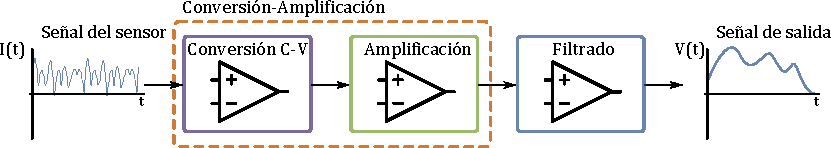
\includegraphics[scale=0.9]{Imagenes/Desarrollo/Dise�oHardware/CAS2.pdf}
	\end{center}
	 \caption{Etapas del CAS para el sensor de OD.} \label{fig:cap3:CAS2}
\end{figure}

Debido a que el sensor de OD, como se describi� en la subsecci�n~\ref{cap2:sec:Sensores:OD}, proporciona una corriente como se�al de salida y el ADC del ATmega8 solo permite voltajes como se�ales de entrada, se requiere el dise�o de un convertidor de corriente a voltaje, como el que se muestra en la figura~\ref{fig:cap3:CVOD} \cite{Cap2Bib:Alexander, Cap2Bib:Hayt}, para acondicionar la se�al.

\begin{figure}[htb]
	\begin{center}
		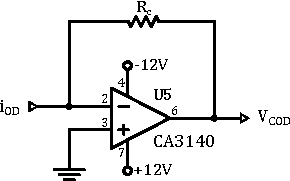
\includegraphics[scale=0.9]{Imagenes/Desarrollo/Dise�oHardware/CASODCV.pdf}
	\end{center}
	\caption{Configuraci�n de la etapa de conversi�n-amplificaci�n .} \label{fig:cap3:CVOD}
\end{figure}

La etapa de amplificaci�n para el CAS del sensor de OD, se incluye en este mismo dise�o, ya que el convertidor de la figura~\ref{fig:cap3:CVOD} se configura para que tenga una ganancia ${G}_{c}={R}_{c}$. Este convertidor de corriente a voltaje se dise�a utilizando la ecuaci�n~\ref{cap3:eq:ODCV}. Debido a que la corriente de la se�al de salida del sensor de OD oscila entre $50\nano\ampere$ y $110\nano\ampere$, se establece una ganancia de conversi�n ${G}_{c}=1*{{10}^{6}}$, con ello se obtiene un voltaje de conversi�n ${V}_{COD}$ que oscila entre $50\milli\volt$ y $110\milli\volt$. Estos niveles de voltaje permitir�n al ADC operar de manera satisfactoria en la toma de mediciones. 

\begin{equation}\label{cap3:eq:ODCV}
{V}_{COD}=-{R}_{c}{i}_{OD}
\end{equation}

donde se tiene que:

\begin{variables}
	\item[${V}_{COD}=$] Voltaje de salida del convertidor.
	\item[${i}_{OD}=$] Corriente del sensor de OD.
	\item[${R}_{c}=$] Resistencia de ganancia de conversi�n.
\end{variables}

Para la etapa de filtrado, se emplea la configuraci�n de un filtro activo pasa-bajas inversor \cite{Cap2Bib:Alexander, Cap2Bib:Coughlin, Cap2Bib:Hayt}. Dicho filtro es de primer orden con ganancia unitaria como el que se muestra en la figura~\ref{fig:cap3:filOD}.

\begin{figure}[htb]
	\begin{center}
		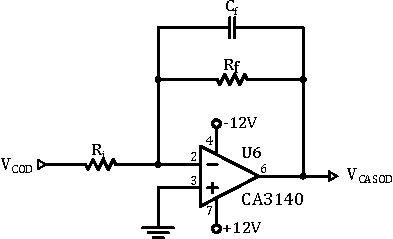
\includegraphics[scale=0.9]{Imagenes/Desarrollo/Dise�oHardware/CASODFiltro.pdf}
	\end{center}
	\caption{Configuraci�n del filtro \emph{pasa-bajas} inversor de ganancia unitaria.} \label{fig:cap3:filOD}
\end{figure}

La frecuencia de corte ${f}_{c}$ de dicho filtro se calcula con la ecuaci�n~\ref{cap3:eq:ODf}.

\begin{equation}\label{cap3:eq:ODf}
{w}_{c}={{1}\over{{R}_{f}{C}_{f}}}=2\pi{f}_{c}
\end{equation}

donde:
\begin{variables}
	\item[${w}_{c}=$] Frecuencia de corte en [$\rad\per\second$].
	\item[${f}_{c}=$] Frecuencia de corte en [$\hertz$].
	\item[${R}_{f}=$] Resistencia de retroalimentaci�n del filtro.
	\item[${C}_{f}=$] Capacitor de retroalimentaci�n del filtro.
	\item[${R}_{i}=$] Resistencia de entrada al filtro, para la ganancia unitaria se hace ${R}_{i}={R}_{f}$.
\end{variables}

La frecuencia de corte de la etapa de filtrado elegida es ${f}_{c}=0.159\hertz$. En la tabla~\ref{tab:cap3:CASOD} se muestran los par�metros para el c�lculo del convertidor de corriente a voltaje y del filtro pasa-bajas y en el ap�ndice~\ref{ap:HWSch} se muestra la configuraci�n completa del CAS del sensor de OD.

\begin{table}[htb]
	\caption{Par�metros usados en el CAS del sensor de OD.}%
	\centering
	\footnotesize
	\begin{tabular}{ccc}
		\hline \hline \hline \hline
		\rowcolor[gray]{0.8}\textbf{Par�metro}&\textbf{Valor}&\textbf{Unidad}\\
		\hline \hline \hline \hline

		${G}_{c}$&$1*{{10}^{6}}$&-\\
		\rowcol	${R}_{c}$&$1$&$\mega\ohm$\\
		${f}_{c}$&$0.159$&$\hertz$\\
		\rowcol	${R}_{f}$&$10$&$\mega\ohm$\\
		${C}_{f}$&$100$&$\nano\farad$\\
		\rowcol	${R}_{i}$&$10$&$\mega\ohm$\\
		\hline \hline \hline \hline
	\end{tabular}
\label{tab:cap3:CASOD}
\end{table}

\newpage
Bas�ndose en el dise�o anterior, el modelo matem�tico del dispositivo CAS para el sensor de OD se describe en la siguiente ecuaci�n:

\begin{equation} \label{cap3:eq:VCASOD}
{V}_{CASOD}=(1*{{10}^{6}})({i}_{OD})
\end{equation}

En la figura~\ref{fig:cap3:SimulacionVCASOD} se ilustra el diagrama esquem�tico empleado en la simulaci�n del CAS para el sensor de OD. En esta simulaci�n se utiliza como entrada una fuente de corriente. Se considera que el dominio del CAS del sensor de OD es una corriente ${I}_{OD}$ que oscila entre $50\nano\ampere$ y $110\nano\ampere$, por lo que en la tabla~\ref{tab:cap4:SimCASOD1} y en la figura~\ref{fig:cap4:GraficaSimulacionCASOD} se muestran los resultados obtenidos de la simulaci�n de manera tabular y gr�fica respectivamente.

\begin{figure}[htb]
	\begin{center}
		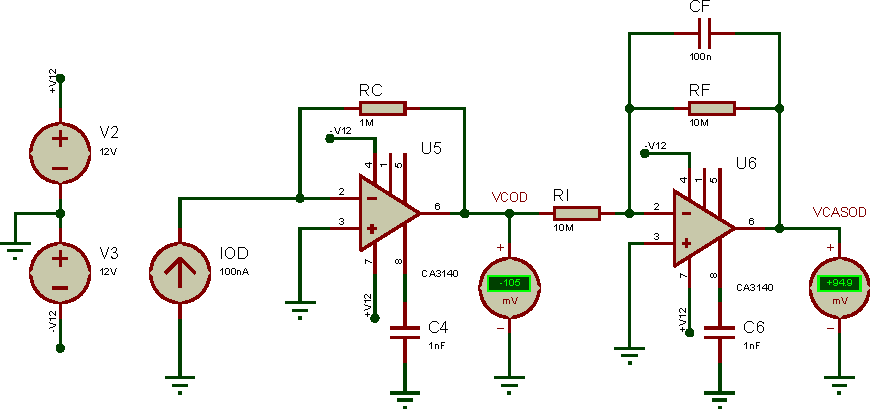
\includegraphics[scale=0.8]{Imagenes/Desarrollo/Dise�oHardware/SimulacionVCASOD.pdf}
	\end{center}
	\caption{Simulaci�n del CAS para el sensor de OD.} \label{fig:cap3:SimulacionVCASOD}
\end{figure}

\begin{table}[htp]
	\caption{Tabla de entradas y salidas de la simulaci�n del CAS para el sensor de OD.}%
	\centering
	\footnotesize
	\begin{tabular}{cc}
		\hline \hline \hline \hline
		\headcol$\pmb{{I}_{OD}}$&$\pmb{{V}_{CASOD}}$\\
		\hline \hline \hline \hline
		$50\nano\ampere$&$44.9\milli\volt$\\
		\rowcol$60\nano\ampere$& $54.9\milli\volt$\\
		$70\nano\ampere$& $64.9\milli\volt$\\
		\rowcol$80\nano\ampere$& $74.9\milli\volt$\\
		$90\nano\ampere$& $84.9\milli\volt$\\
		\rowcol$100\nano\ampere$& $94.9\milli\volt$\\
		$110\nano\ampere$& $105.9\milli\volt$\\
		\hline \hline \hline \hline
	\end{tabular}
	\label{tab:cap4:SimCASOD1}
\end{table}
\newpage
\begin{center}
	\pgfplotsset{every axis/.append style={thick,tick style={thin},font=\footnotesize}}
\begin{tikzpicture}
\tikzset{
every pin/.style={fill=yellow!50!white,rectangle,rounded corners=3pt,font=\scriptsize},
small dot/.style={fill=black,circle,scale=0.3}
}
	\begin{axis}[use units,x=0.075cm,y=0.075cm,
			minor tick num=3,
			axis y line=middle,
			axis x line=middle,
			x unit=nA,xlabel=${I}_{OD}$,
			y unit=mV,ylabel=${V}_{CASOD}$
		]
		\addplot[smooth,teal] table[x={iod}, y={vcasod}]{CASODSimulation.data};
	\end{axis}
\end{tikzpicture}



	\captionof{figure}{Gr�fica de entradas y salidas de la simulaci�n del CAS para el sensor de OD.} \label{fig:cap4:GraficaSimulacionCASOD}
\end{center}


\paragraph{CAS del sensor de temperatura}

El dise�o del CAS del sensor de temperatura se dividi� en las etapas de aislamiento, filtrado y amplificaci�n (Figura~\ref{fig:cap3:CAS1}).

\begin{figure}[htb]
	\begin{center}
		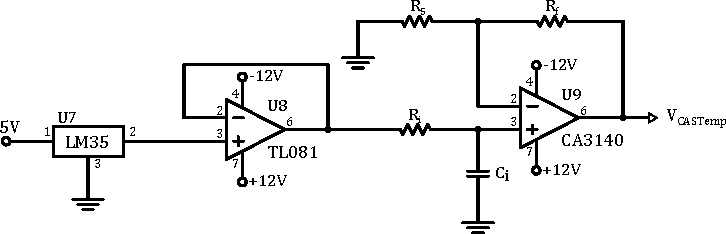
\includegraphics[scale=0.9]{Imagenes/Desarrollo/Dise�oHardware/CASTemp.pdf}
	\end{center}
	 \caption{Configuraci�n del CAS para el sensor de temperatura.} \label{fig:cap3:CASTemp}
\end{figure}

La etapa de aislamiento emplea la configuraci�n de un seguidor de voltaje (figura~\ref{fig:cap3:CASTemp}), en donde se obtiene un voltaje de salida ${V}_{temp}$ que es proporcional a la temperatura ambiente con una sensibilidad de $10\milli\volt\per\degreecelsius$.

Para la etapa de filtrado y amplificaci�n se emplea la misma configuraci�n usada para el sensor de pH (figura~\ref{fig:cap3:CASTemp}), la frecuencia de corte del filtro seleccionada es ${f}_{c}=1.59\hertz$ y para una mejor resoluci�n del m�dulo ADC del ATmega8 se eligi� una ganancia de amplificaci�n ${G}_{a}=4$. En la tabla~\ref{tab:cap3:CAStemp} se muestran los par�metros utilizados para el c�lculo del filtro y el amplificador.

\begin{table}[htp]
	\caption{Par�metros usados en el CAS del sensor de temperatura.}%
	\centering
	\footnotesize
	\begin{tabular}{ccc}
		\hline \hline \hline \hline
		\rowcolor[gray]{0.8}\textbf{Par�metro}&\textbf{Valor}&\textbf{Unidad}\\
		\hline \hline \hline \hline

		${R}_{i}$&$1$&$\mega\ohm$\\
		\rowcol ${C}_{i}$&$100$&$\nano\farad$\\
		${f}_{c}$&$1.59$&$\hertz$\\
		\rowcol ${R}_{f}$&$47$&$\kilo\ohm$\\
		${R}_{5}$&$15$&$\kilo\ohm$\\
		\rowcol ${G}_{a}$&$4$&-\\
		\hline \hline \hline \hline
	\end{tabular}
	\label{tab:cap3:CAStemp}
\end{table}

Del dise�o anterior, el modelo matem�tico del dispositivo CAS para el sensor de temperatura se describe en la siguiente ecuaci�n:

\begin{equation} \label{cap3:eq:VCASTemp}
{V}_{CASTemp}=4*{V}_{temp}
\end{equation}

\newpage
En la figura~\ref{fig:cap3:SimulacionVCASTemp} se muestra la simulaci�n del CAS para el sensor de temperatura y el diagrama esquem�tico empleado. Se considera que el dominio de dicho CAS es un voltaje ${V}_{Temp}$, el cual est� en funci�n de la temperatura ambiente, por lo que presenta una sensibilidad de $10\milli\volt \per \degreecelsius$. En la figura~\ref{fig:cap4:SimCASTemp} y en la tabla~\ref{tab:cap4:SimulacionCASTemp} se muestran los resultados obtenidos de la simulaci�n de manera gr�fica y tabular respectivamente.

\begin{figure}[htb]
	\begin{center}
		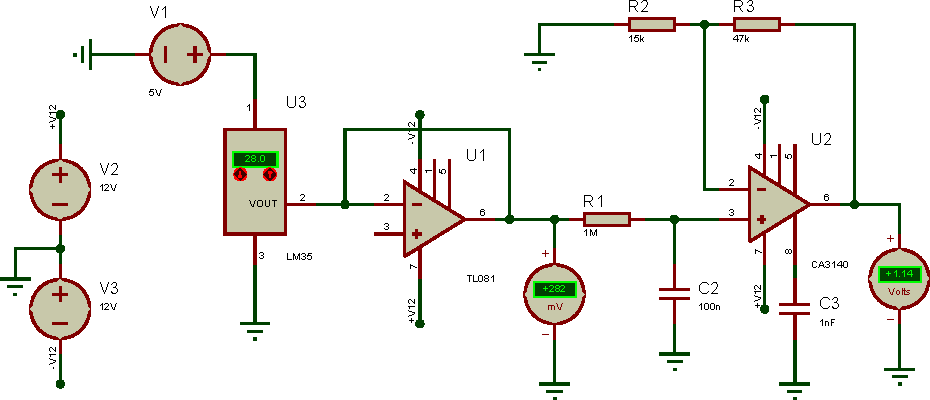
\includegraphics[scale=0.85]{Imagenes/Desarrollo/Dise�oHardware/SimulacionVCASTemp.pdf}
	\end{center}
	\caption{Simulaci�n del CAS para el sensor de temperatura.} \label{fig:cap3:SimulacionVCASTemp}
\end{figure}

\begin{center}
	\pgfplotsset{every axis/.append style={thick,tick style={thin},font=\footnotesize}}
\begin{tikzpicture}
\tikzset{
every pin/.style={fill=yellow!50!white,rectangle,rounded corners=3pt,font=\scriptsize},
small dot/.style={fill=black,circle,scale=0.3}
}
	\begin{axis}[use units,x=0.1cm,y=15cm,
			minor tick num=3,
			axis y line=middle,
			axis x line=middle,
			x unit=mV,xlabel=${V}_{Temp}$,
			y unit=V,ylabel=${V}_{CASTemp}$
		]
		\addplot[smooth,teal] table[x={vtemp}, y={vcastemp}]{CASTempSimulation.data};
	\end{axis}
\end{tikzpicture}



	\captionof{figure}{Gr�fica de entradas y salidas de la simulaci�n del CAS para el sensor de temperatura.} \label{fig:cap4:SimCASTemp}
\end{center}

\begin{table}[htp]
	\caption{Tabla de entradas y salidas de la simulaci�n del CAS para el sensor de temperatura.}%
	\centering
	\footnotesize
	\begin{tabular}{cc}
		\hline \hline \hline \hline
		\headcol$\pmb{{V}_{Temp}}$&$\pmb{{V}_{CASTemp}}$\\
		\hline \hline \hline \hline
		$272\milli\volt$ & $1.10\volt$\\
		\rowcol $282\milli\volt$ & $1.14\volt$\\
		$292\milli\volt$ & $1.18\volt$\\
		\rowcol $302\milli\volt$ & $1.23\volt$\\
		$312\milli\volt$ & $1.27\volt$\\
		\rowcol $322\milli\volt$ & $1.31\volt$\\
		\hline \hline \hline \hline
	\end{tabular}
	\label{tab:cap4:SimulacionCASTemp}
\end{table}


\subsubsection{Entradas y salidas de la RTU}
\label{cap3:DHW:RTUES}
Para el dise�o hardware de la RTU se definen las entradas y salidas del MCU ATmega8 (figura~\ref{fig:cap3:RTU}) \cite{Cap2Bib:ATmega8}. Como entradas se tienen a las se�ales de los sensores y entradas digitales, y las salidas son la alimentaci�n del sensor de OD y las salidas digitales. 

\begin{figure}[htb]
	\begin{center}
		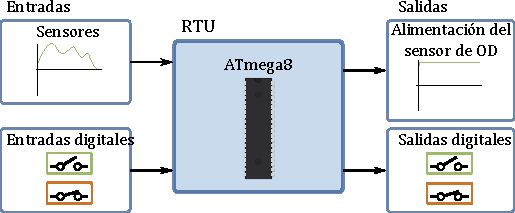
\includegraphics[scale=0.9]{Imagenes/Desarrollo/Dise�oHardware/RTU.pdf}
	\end{center}
	\caption{Configuraci�n de la RTU.} \label{fig:cap3:RTU}
\end{figure}

%\newpage
El voltaje de alimentaci�n del sensor de OD se genera empleando el DAC0808, en donde el nivel de voltaje de salida se establece a trav�s de un c�digo binario contenido en un registro de entrada de 8 bits, el cual es generado por el ATmega8.

%\newpage
Las terminales del ATmega8 se distribuyen en cuatro �reas (figura~\ref{fig:cap3:ATmega8DT}): las entradas anal�gicas (se�ales de los sensores) que hacen uso de los canales ADC0-ADC2, la entrada y salida de datos serie a trav�s de las terminales RXD y TXD respectivamente, las entradas y salidas digitales utilizan los puertos PD2-PD3 y PD4-PD5 respectivamente, y el registro de salida que indica el nivel de voltaje de alimentaci�n para el sensor de OD utiliza el puerto B (PB0-PB7).

\begin{figure}[htb]
	\begin{center}
		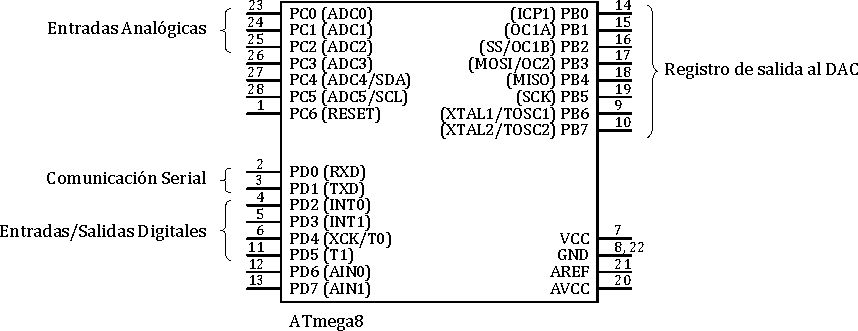
\includegraphics[scale=0.9]{Imagenes/Desarrollo/Dise�oHardware/ATmega8DT.pdf}
	\end{center}
	 \caption{Distribuci�n de terminales del ATmega8.} \label{fig:cap3:ATmega8DT}
\end{figure}

La configuraci�n empleada para el DAC0808 se muestra en la figura~\ref{fig:cap3:DACConf}, la cual proporciona un voltaje de salida ${V}_{POD}$ con una resoluci�n de $4.18\milli\volt\per$bit \cite{Cap2Bib:DAC0808}.

\begin{figure}[htb]
	\begin{center}
		\includegraphics[scale=0.9]{Imagenes/Desarrollo/Dise�oHardware/DACConf.pdf}
	\end{center}
	 \caption{Configuraci�n del DAC0808.} \label{fig:cap3:DACConf}
\end{figure}

%\newpage
\subsubsection{Interfaz RS-485}
\label{cap3:DHW:RS485}
Para la comunicaci�n de la RTU con la MTU se emplea una interfaz RS-485 como medio f�sico. Dicha interfaz se implementa utilizando el dispositivo USART que incluye el MCU, el cual se conecta al dispositivo MAX489 para implementar una l�nea de transmisi�n balanceada.

%\newpage
La configuraci�n empleada para el dise�o de la interfaz RS-485 se muestra en la figura~\ref{fig:cap3:MAX489Conf} \cite{Cap2Bib:MAX489}, en donde se utilizan los puertos RXD/TXD del ATmega8 para la recepci�n/transmisi�n de datos series mediante el dispositivo USART y el dispositivo MAX489 se configura para la operaci�n en modo \emph{full-duplex}.

\begin{figure}[htb]
	\begin{center}
		\includegraphics[scale=0.9]{Imagenes/Desarrollo/Dise�oHardware/MAX489Conf.pdf}
	\end{center}
	\caption{Configuraci�n del dispositivo MAX489.} \label{fig:cap3:MAX489Conf}
\end{figure}


\subsubsection{Transceptor RS-232/RS-485}
\label{cap3:DHW:RS232RS485}

La MTU (computadora) cuenta con un puerto serie cuyo funcionamiento est� basado en el est�ndar RS-232, debido a esto, para comunicar la MTU con la RTU es necesario implementar un transceptor RS-232/RS-485 (figura~\ref{fig:cap3:RTU-MTU}). 

\begin{figure}[htb]
	\begin{center}
		\includegraphics[scale=0.9]{Imagenes/Desarrollo/Dise�oHardware/RTU-MTU.pdf}
	\end{center}
	\caption{Comunicaci�n serie de la RTU con la MTU.} \label{fig:cap3:RTU-MTU}
\end{figure}

%\newpage
El transceptor RS-232/RS-485 se divide en dos etapas, la primer etapa consiste en obtener los datos serie de la interfaz RS-485 en niveles TTL, lo cual se realiza empleando el dispositivo MAX489; y, la segunda etapa convierte los niveles TTL a voltajes del est�ndar RS-232, lo cual se realiza utilizando el dispositivo MAX232.

El dispositivo MAX489 se configura para operar en modo \emph{full-duplex} y la configuraci�n empleada para el dispositivo MAX232 utiliza capacitores externos para su funcionamiento \cite{Cap2Bib:MAX489, Cap2Bib:MAX232}. Dicha configuraci�n se ilustra en la figura~\ref{fig:cap3:Pasarela}.

\begin{figure}[htb]
	\begin{center}
		\includegraphics[scale=.95]{Imagenes/Desarrollo/Dise�oHardware/Pasarela485-232.pdf}
	\end{center}
	 \caption{Transceptor RS-232/RS-485.} \label{fig:cap3:Pasarela}
\end{figure}


\newpage
\subsection{Dise�o \emph{software}}
\label{cap3:Definicion:DSW}
% Procurar que se empiece una nueva p�gina
El desarrollo del sistema se divide en tres etapas \emph{Software} (Tabla~\ref{tab:cap3:Thwsw}, ). El dise�o de estas etapas se realiz� empleando el Lenguaje Unificado de Modelado (UML, \emph{Unified Modeling Language}). Las etapas \emph{software} se describen a continuaci�n:

\begin{itemize} \itemsep=-0.5em
	\item \emph{Software de la RTU}: En esta etapa se detalla el dise�o \emph{software} del MCU ATmega8. Con este \emph{software}, el MCU implementar� una RTU empleando el protocolo Modbus. El desarrollo se realizar� en lenguaje C.
	\item\emph{Software de la MTU}: Esta etapa describe a detalle el dise�o del \emph{software} de la MTU. La MTU de Modbus ser� implementada en una computadora. Este \emph{software} se implementar� en lenguaje Java.
	\item\emph{Software de la aplicaci�n Web}: Describe el dise�o de la aplicaci�n Web en base a los requerimientos establecidos. Se emplear� el framework Yii y una base de datos MySQL.
\end{itemize}

\subsubsection{\emph{software} de la RTU}

\paragraph{Requerimientos formales}
En base a los requerimientos funcionales de la propuesta, se obtuvieron de manera concreta los requerimientos formales de las tareas que debe desempe�ar el \emph{software} de la RTU. Dichos requerimientos formales se describen en la tabla~\ref{tab:cap3:ReqRTU} y en la figura~\ref{fig:cap3:ReqRTU} se ilustra la relaci�n entre los requerimientos mediante un diagrama de requerimientos.

\begin{table}[htp]
	\caption{Requerimientos formales del \emph{software} de la RTU.}%
	\centering
	\footnotesize
	\begin{tabular}{clp{8cm}}
		\hline \hline \hline \hline
		\headcol\textbf{C�digo}&\textbf{Requerimiento}&\textbf{Descripci�n}\\
		\hline \hline \hline \hline
		
		REQ01	&	Procesamiento de Solicitudes de la MTU & Procesar las solicitudes o ADUs (Protocolo Modbus) que emite la MTU para monitorear el estado de la RTU.\\
		\rowcol REQ02 & Adquisici�n de datos a trav�s del ADC & Consiste en configurar el ADC para tomar la lectura de los sensores.\\
		REQ03 & Obtenci�n de Estados Digitales & Para obtener los estados de las Entradas y Salidas Digitales.\\
		\rowcol REQ04 & Construir y	enviar respuesta a la MTU & Consiste en construir una ADU de respuesta a una solicitud emitida por la MTU.\\
		REQ05 & Establecer Salidas Digitales & Establecer las Salidas Digitales de acuerdo a los par�metros de las solicitudes de la MTU.\\

		\hline \hline \hline \hline		
	\end{tabular}
	\label{tab:cap3:ReqRTU}
\end{table}
 
\begin{figure}[htb]
	\begin{center}
		\includegraphics[scale=0.85]{Imagenes/Desarrollo/Dise�oSW/RTUReqForm.pdf}
	\end{center}
	 \caption{Diagrama de requerimientos formales del \emph{software} de la RTU.}\label{fig:cap3:ReqRTU}
\end{figure}

\paragraph{Clases}

El \emph{software} de la RTU consta de cuatro m�dulos principales (Figura~\ref{fig:cap3:RTUModulos}): gesti�n del dispositivo ADC, puertos digitales de Entrada y Salida, gesti�n del dispositivo USART y el \emph{software} principal de procesamiento de ADUs de solicitud emitidas por la MTU. La estructura \emph{software} de la RTU consiste de una sola clase llamada RTU que se ilustra en la figura~\ref{fig:cap3:RTUClass}. 

\begin{figure}[htb]
	\begin{center}
		\begin{tabular}{cc}
			\subfloat[M�dulos del \emph{software} de la RTU.]{%
				\label{fig:cap3:RTUModulos}%
				\includegraphics[scale=0.9]{Imagenes/Desarrollo/Dise�oSW/ATmega8Modulos.pdf}} &
			\subfloat[Clase RTU.]{%
				\label{fig:cap3:RTUClass}%
				\includegraphics[scale=0.9]{Imagenes/Desarrollo/Dise�oSW/RTUClass.pdf}} \\
		\end{tabular}
	\end{center}
	\caption{Estructura \emph{software} de la RTU.} \label{fig:cap3:StSWRTU}
\end{figure}

La clase RTU consiste de siete operaciones o m�todos que se describen en la tabla~\ref{tab:cap3:RTUOp}. Estos m�todos contribuyen a que la RTU desempe�e de manera modular las actividades programadas.

\begin{table}[htp]
	\caption{Operaciones de la clase RTU.}%
	\centering
	\footnotesize
	\begin{tabular}{cp{11.5cm}}
		\hline \hline \hline \hline
		\headcol\textbf{C�digo de Operaci�n}&\textbf{Descripci�n}\\
		\hline \hline \hline \hline
		
		CadSend & Se encarga de enviar las ADU de respuesta (ya construidas) a la interfaz serie del MCU.\\
		\rowcol Crc16Modbus & Construye el c�digo de verificaci�n CRC, los par�metros de entrada son: la ADU a enviar (sin CRC) y el tama�o de la misma. Retorna el c�digo CRC en 16 bits en un tipo de dato entero, pero se tomar�n solo los valores en codificaci�n Hexadecimal.\\
		DecodeFrame & Decodifica las ADU de entrada y ejecuta las acciones de toma de mediciones, obtenci�n de estados digitales y establecer salidas digitales.\\
		\rowcol initUSART & Establece la configuraci�n inicial del dispositivo serie (USART) del MCU.\\
		ISR(USART\_RXC\_vect) & Configura las operaciones que se realizar�n al recibir informaci�n a trav�s del puerto serie. La ejecuci�n de estas operaciones dependen del disparador por eventos en la recepci�n de informaci�n en el dispositivo USART (Interrupciones).\\
		\rowcol SensorsRead & Toma muestras de los sensores a trav�s del dispositivo ADC.\\

		\hline \hline \hline \hline		
	\end{tabular}
	\label{tab:cap3:RTUOp}
\end{table}


\paragraph{Diagramas de actividades}
\label{cap3:DSW:RTUDA}
En este apartado se detallan los flujos de trabajo de las actividades y operaciones que el \emph{software} de la RTU debe realizar. Para la RTU se dividen sus actividades \emph{software} en dos partes funcionales: inicializaci�n de m�dulos y procesamiento de ADUs de solicitud.

La inicializaci�n de m�dulos consiste en configurar los m�dulos principales de la RTU (MCU ATmega8) que se muestran en la figura~\ref{fig:cap3:RTUModulos}. Por esto, se configuran los puertos de entrada y salida\footnote{Cada m�dulo del MCU ATmega8 utiliza puertos de entrada y salida para interactuar con dispositivos externos.} y registros internos\footnote{Los registros internos se utilizan para configurar el modo de operaci�n de cada m�dulo: ADC, USART, etc.} de configuraci�n \cite{Cap2Bib:ATmega8}. Estas tareas se ejecutan cada vez que se inicia el sistema o cuando ocurre un reset de la RTU.

El diagrama de actividades de la figura~\ref{fig:cap3:RTUInicializacion} describe la inicializaci�n de m�dulos mediante cuatro acciones: inicializar puertos digitales de Entrada y Salida, inicializar el dispositivo USART y habilitar las interrupciones globales para eventos en la USART\footnote{Las interrupciones de eventos en la USART permiten ejecutar un fragmento de c�digo cuando un dato est� disponible en el b�fer de entrada.} \cite{Cap2Bib:ATmega8}.

\begin{figure}[H]
	\begin{center}
		\begin{tabular}{c@{\hskip 0.5in}c}
			\subfloat[Inicializaci�n de m�dulos del \emph{software} de la RTU.]{%
				\label{fig:cap3:RTUInicializacion}%
				\includegraphics[scale=0.85]{Imagenes/Desarrollo/Dise�oSW/RTUInicializacion.pdf}} &
			\subfloat[Procesamiento de ADUs de solicitud.]{%
				\label{fig:cap3:RTUProcesamiento}%
				\includegraphics[scale=0.85]{Imagenes/Desarrollo/Dise�oSW/RTUProcesamiento.pdf}} \\
		\end{tabular}
	\end{center}
	\caption{Diagramas de actividades del \emph{software} de la RTU} \label{fig:cap3:SWRTUDA}
\end{figure}

La configuraci�n de los dispositivos del MCU ATmega8 se describe en la tabla~\ref{tab:cap3:RTUDConf} \footnote{El Oscilador interno RC es una fuente de reloj que provee las siguientes frecuencias calibradas de operaci�n: $1.0$, $2.0$, $4.0$, y $8.0\mega\hertz$. La configuraci�n del dispositivo USART aplica en general para la comunicaci�n serie, es decir, para la interfaz RS-232 y RS-485.} \cite{Cap2Bib:ATmega8}. 

\begin{table}[htp]
	\caption{Configuraci�n de dispositivos del MCU ATmega8.}%
	\centering
	\footnotesize
	\begin{tabular}{clp{8cm}}
		\hline \hline \hline \hline
		\headcol\textbf{Dispositivo}&\textbf{Par�metro}&\textbf{Descripci�n}\\
		\hline \hline \hline \hline
		
		Oscilador interno RC & $f_{o} = 4\mega\hertz$ & Se configur� para obtener una fuente de reloj de operaci�n de $f_{o} = 4\mega\hertz$. Por lo tanto, $f_{o}$ garantiza satisfacer la demanda en la velocidad de transferencia de la interfaz serie (dispositivo USART).\\
		
		\rowcol Dispositivo ADC & ${f_{ADC}} = {f_{o}}/{32} = 125\kilo\hertz$ & La frecuencia de operaci�n del ADC requiere una fuente de reloj de $50-200 \kilo\hertz$.\\
		
		\multirow{6}{*}{Dispositivo USART} & Velocidad de transferencia & $38400$bps\\
		& Tama�o de datos & 8 bits\\
		& Paridad & Par\\
		& Bits de paro & Uno\\
		& Modo de Operaci�n & As�ncrono\\
		& Interrupciones & Por recepci�n de datos\\
		
		\hline \hline \hline \hline		
	\end{tabular}
	\label{tab:cap3:RTUDConf}
\end{table}

En base a la distribuci�n de terminales del MCU ATmega8 que se muestra en la figura~\ref{fig:cap3:ATmega8DT}, la configuraci�n de terminales se describe en la tabla~\ref{tab:cap3:RTUTConf} \cite{Cap2Bib:ATmega8}.

\begin{table}[htp]
	\caption{Configuraci�n de terminales del MCU ATmega8.}%
	\centering
	\footnotesize
	\begin{tabular}{clp{9.5cm}}
		\hline \hline \hline \hline
		\headcol\textbf{Terminales}&\textbf{Configuraci�n}&\textbf{Descripci�n}\\
		\hline \hline \hline \hline

		PC0-PC3 & Entrada & Terminales usadas como canales de entrada del dispositivo ADC\\
		\rowcol PD2-PD3 & Entrada & Entradas digitales\\
		PD4-PD5 & Salida & Salidas digitales\\
		\rowcol Puerto B (PB0-PB7)& Salida & Registro de salida para generar el voltaje de polarizaci�n del sensor de OD a trav�s del dispositivo DAC.\\
		PD0-PD1 & Entrada/Salida & Terminales para recepci�n y transmisi�n de datos desde y hacia el dispositivo USART.\\
		\hline \hline \hline \hline		
	\end{tabular}
	\label{tab:cap3:RTUTConf}
\end{table}

El procesamiento de ADUs de solicitud define las actividades y el orden en que se deben realizar para atender las solicitudes que emite la MTU. Dichas actividades son: verificar si se ha recibido una ADU a trav�s del dispositivo USART, validar que sea una ADU consistente, decodificar la ADU\footnote{Solo si la ADU es v�lida.} con el fin de realizar la tarea solicitada y enviar una respuesta, si se trata de una ADU inv�lida se enviar� un c�digo de error. Este flujo de trabajo se ilustra en el diagrama de actividades de la figura~\ref{fig:cap3:RTUProcesamiento}.

Como se observa en la figura~\ref{fig:cap3:RTUProcesamiento}, para comprobar que hay una ADU de entrada el \emph{software} entra en un bucle \emph{while }, se reciben datos a trav�s del dispositivo USART\footnote{El dispositivo USART emite una interrupci�n cada vez que se recibe un \emph{byte} de informaci�n.}, mediante una bandera se indica cuando la ADU ha sido recibida en su totalidad y posteriormente se procesa la ADU. Se comprueba que la ADU sea v�lida, lo cual se realiza verificando el c�digo CRC y en caso de un error en esta verificaci�n se retorna un c�digo de error. Despu�s, se ejecuta la tarea solicitada\footnote{Leer entradas anal�gicas, obtener el estado de entradas y salidas digitales, establecer salidas digitales.}, se construye la ADU de respuesta y por �ltimo se env�a la ADU de respuesta a la MTU a trav�s del dispositivo USART.

\newpage
\subsubsection{\emph{software} de la MTU}
\label{cap3:DSWMTU}
\paragraph{Requerimientos formales}

Los requerimientos formales de las tareas \emph{software} de la MTU (obtenidos a partir de los requerimientos funcionales de la propuesta) se describen en la tabla~\ref{tab:cap3:ReqMTU} y el diagrama de requerimientos de la figura~\ref{fig:cap3:MTUReqForm} ilustra la relaci�n entre dichos requerimientos.

\begin{table}[htp]
	\caption{Requerimientos formales del \emph{software} de la MTU}%
	\centering
	\footnotesize
	\begin{tabular}{cp{5cm}p{8.5cm}}
		\hline \hline \hline \hline
		\headcol\textbf{C�digo}&\textbf{Requerimiento}&\textbf{Descripci�n}\\
		\hline \hline \hline \hline
		
		REQ06 & Monitorizaci�n autom�tica de la RTU & Realizar las actividades de monitoreo discreto de la RTU a trav�s de ADUs de solicitud, el monitoreo se debe realizar cada determinado tiempo establecido por el usuario\\
		\rowcol REQ07 & Gesti�n del b�fer de entrada y salida al puerto RS-232 & Gestionar de manera eficiente el b�fer de entrada y salida del puerto RS-232\\
		REQ08 & Recepci�n y procesamiento de ADUs de respuesta de la RTU & Procesar las ADUs que la RTU env�a como respuesta ante una solicitud de monitoreo discreto\\
		\rowcol REQ09 & Almacenamiento de mediciones y estados digitales en la Base de Datos & Realizar los c�lculos pertinentes en la medici�n de cada sensor\footnote{La RTU solo env�a la medici�n anal�gica de cada sensor, por lo que el \emph{software} de la MTU debe calcular los valores propios del par�metro medido. Esto se realiza en base a la descripci�n de los sensores de la secci�n~\ref{cap2:sec:Sensores}.} y almacenar los resultados en la base de datos\\
		REQ10 & Procesamiento de Solicitudes recibidas v�a TCP/IP para establecer salidas digitales & Procesar las solicitudes enviadas a trav�s de la aplicaci�n Web para establecer el estado de las salidas digitales, estas solicitudes son enviadas por el usuario final o Administrador del sistema\\
		\rowcol REQ11 & Gesti�n f�sica del puerto RS-232 & Utilizar una librer�a para gestionar el uso de la interfaz serie RS-232 en un nivel f�sico, es decir, que permita configurar la interfaz serie con las especificaciones\\
		REQ12 & Calibraci�n de sensores & Calibrar los sensores de pH y OD mediante la toma de mediciones a muestras fijas.\\
		\hline \hline \hline \hline		
	\end{tabular}
	\label{tab:cap3:ReqMTU}
\end{table}

\begin{figure}[htb]
	\begin{center}
		\includegraphics[scale=0.85]{Imagenes/Desarrollo/Dise�oSW/MTUReqForm.pdf}
	\end{center}
	\caption{Diagrama de requerimientos formales del \emph{software} de la MTU.} \label{fig:cap3:MTUReqForm}
\end{figure}

\newpage
\paragraph{Clases}

Para gestionar correctamente las entradas y salidas de la interfaz serie (Puerto RS-232), el \emph{software} de la MTU se basa en el \emph{Modelo del Gestor}\footnote{En programaci�n, el Modelo del Gestor consiste en un proceso central que crea, ejecuta y administra un grupo de subprocesos (Thread Pool).}, el cual es un modelo de control centralizado para sistemas concurrentes \cite{Cap2Bib:Java}. Por ello, para un mejor desempe�o, el \emph{software} de la MTU se divide en m�ltiples tareas que se ejecutan de manera concurrente. Esto se logra mediante la programaci�n de m�ltiples hilos o subprocesos de ejecuci�n (\emph{Multithreading}) \cite{Cap2Bib:Java}.

Bas�ndose en el \emph{Modelo del Gestor} y los requerimientos funcionales, los subprocesos en que se divide el \emph{software} de la MTU son: subprocesos de monitoreo discreto de la RTU, un gestor del b�fer de entrada y salida del puerto serie (RS-232), procesador de ADUs de respuesta de la RTU, subproceso para almacenar registros de mediciones y estados digitales en la base de datos, un servidor TCP/IP para recibir solicitudes emitidas desde la aplicaci�n Web y el manejador de eventos de la interfaz gr�fica\footnote{El manejador de eventos es un mecanismo que se genera al crear una interfaz gr�fica en Java.}. En la figura~\ref{fig:cap3:SWMTUModeloGestor} se ilustra en un diagrama el Modelo del Gestor para el \emph{software} de la MTU.

\begin{figure}[htb]
\begin{center}
 \includegraphics[scale=0.9]{Imagenes/Desarrollo/Dise�oSW/SWMTUModeloGestor.pdf}
\end{center}
 \caption{Divisi�n de subprocesos del \emph{software} de la MTU.} \label{fig:cap3:SWMTUModeloGestor}
\end{figure}

Los subprocesos de monitoreo de la RTU implementan las funciones del protocolo Modbus y generan las ADUs de cada funci�n. Por esto, se crea un subproceso para cada funci�n usada en el sistema propuesto. Los subprocesos emiten solicitudes o ADUS de monitoreo cada cierto tiempo determinado (Tiempo de muestreo\footnote{El tiempo de muestreo lo establece el usuario o Administrador.}), por lo que, el resto del tiempo el subproceso pasa a un estado temporalmente fuera de ejecuci�n (\emph{Sleep}). 

Los subprocesos requieren acceso al b�fer de salida del puerto serie de manera espor�dica\footnote{No se puede determinar el orden en el que los subprocesos cambian su estado a \emph{ejecuci�n}.} para enviar las ADUs de solicitud. Por todo lo anterior, se presenta el problema de programaci�n conocido como la relaci�n \emph{productor-consumidor}, en donde el productor genera datos y los almacena en un objeto compartido, y los consumidores leen los datos de dicho objeto. 

El objeto compartido se denomina \emph{B�fer Sincronizado}, el cual restringe el acceso a la interfaz serie de salida (b�fer de salida) a solo un subproceso de monitoreo (Productor\footnote{En este sistema, el productor es un sistema compuesto que consiste de los subprocesos de monitoreo y las respuestas la RTU.}) a la vez y se implementa una cola de espera para que los subprocesos puedan acceder a �l de manera ordenada. De manera similar, el b�fer de entrada restringe al subproceso que decodifica ADUs de respuesta (Consumidor) para que pase a un estado \emph{sleep} hasta que una respuesta este disponible en el b�fer \cite{Cap2Bib:Java}.

Las clases en que se divide el \emph{software} de la MTU se describen en el ap�ndice~\ref{ap:SWMTU:Class}, en donde se muestran los diagramas de clase para ilustrar la relaci�n entre ellas. Los diagramas de clase se dividen en cuatro secciones: monitoreo de entradas anal�gicas, monitoreo de entradas digitales, diagrama de monitoreo y control de salidas digitales y calibraci�n de sensores.

Cabe mencionar que, para poder usar el puerto serie de la computadora, el \emph{software} de la MTU emplea el \emph{Driver} de la marca \emph{Giovynet}\footnote{El \emph{Driver Giovynet} es un framework que permite crear aplicaciones Java y comunicar circuitos externos y la computadora. Se puede descargar la versi�n gratuita de prueba desde \href{http://www.giovynet.com}{http://www.giovynet.com}.}. Y para acceder a la base de datos desde el \emph{software} de la MTU se usa el driver \emph{JDBC} (\emph{Java Database Connectivity}).

\paragraph{Casos de uso}

Para satisfacer los requerimientos formales del \emph{software} de la MTU, los casos de uso que se dise�aron de acuerdo a la interacci�n del Administrador con el \emph{software} para realizar las siguientes actividades\footnote{Actividades del Administrador.}: monitoreo principal y calibraci�n de sensores. 

El monitoreo principal consiste en iniciar y configurar el \emph{software} de la MTU, el cual de manera autom�tica crea y ejecuta los subprocesos de monitoreo y permite al Administrador configurar el tiempo de muestreo para cada subproceso de monitoreo. Los casos de uso para las actividades de monitoreo principal se detallan en la tabla~\ref{tab:cap3:MTUCUMonitor} y en la figura~\ref{fig:cap3:MTUCUMonitor} se ilustra la interacci�n con el Administrador.

\begin{table}[htp]
	\caption{Casos de uso del monitoreo principal.}%
	\centering
	\footnotesize
	\begin{tabular}{cp{5cm}p{8.3cm}}
		\hline \hline \hline \hline
		\headcol\textbf{C�digo}&\textbf{Caso de uso}&\textbf{Descripci�n}\\
		\hline \hline \hline \hline
		
		CU1 & Inicio del sistema de monitoreo & El Administrador inicia el \emph{software} de la MTU.\\
		
		\rowcol CU2 & Inicializar Subprocesos de Monitoreo y Control de la RTU & El proceso central del \emph{software} de la MTU, en su papel de gestor, crea e inicia los subprocesos de monitoreo.\\
		
		CU3 & Establecer tiempo de muestreo para Entradas Anal�gicas & El \emph{software} permite al Administrador cambiar el tiempo de muestreo del subproceso de monitoreo para entradas anal�gicas.\\
		
		\rowcol CU4 & Establecer tiempo de muestreo para Entradas Digitales & El \emph{software} permite al Administrador configurar el tiempo de muestreo para el subproceso de monitoreo para entradas digitales\\
		
		CU5 & Establecer tiempo de muestreo para Salidas Digitales & El Administrador puede cambiar el tiempo de muestreo del subproceso de monitoreo para salidas digitales.\\
		
		\rowcol CU6 & Establecer Salidas Digitales & Permite al Administrador establecer el estado (\emph{ON-OFF}) de las salidas digitales.\\

		\hline \hline \hline \hline		
	\end{tabular}
	\label{tab:cap3:MTUCUMonitor}
\end{table}

\begin{figure}[htb]
\begin{center}
 \includegraphics[scale=0.85]{Imagenes/Desarrollo/Dise�oSW/MTUCUMonitor.pdf}
\end{center}
 \caption{Casos de uso para monitoreo principal.} \label{fig:cap3:MTUCUMonitor}
\end{figure}

La calibraci�n de sensores define las actividades que el usuario debe realizar con el fin de realizar satisfactoriamente la calibraci�n de los sensores de pH y OD. Para el sensor de pH se requiere como par�metro el valor de la muestra de pH que se va a medir, los valores por defecto establecen la calibraci�n de f�brica (Considerando el comportamiento descrito en la secci�n~\ref{cap2:Sensores:pH}) y el sensor de OD requiere la presi�n barom�trica\footnote{La presi�n barom�trica est� en funci�n de la altitud del lugar donde se tomar� la medici�n.}. En la tabla~\ref{tab:cap3:MTUCUCalibracion} se describen los casos de uso y en la figura~\ref{fig:cap3:MTUCUCalibracion} se ilustra la interacci�n con el Administrador.

\begin{table}[H]
	\caption{Casos de uso de la calibraci�n de sensores.}%
	\centering
	\footnotesize
	\begin{tabular}{cp{5cm}p{8.3cm}}
		\hline \hline \hline \hline
		\headcol\textbf{C�digo}&\textbf{Caso de uso}&\textbf{Descripci�n}\\
		\hline \hline \hline \hline
		
		CU7 & Insertar par�metros de calibraci�n (si son requeridos) & El usuario puede ingresar los par�metros necesarios para realizar la calibraci�n de un sensor.\\
		
		\rowcol CU8 & Toma de mediciones de las muestras & El \emph{software} indicar� al subproceso de monitoreo de entradas anal�gicas que la medici�n que la pr�xima medici�n se tomar� para calibraci�n.\\
		
		CU9 & Realizar calibraci�n en el sistema & Se realizar� la calibraci�n de acuerdo a la medici�n que se halla tomado.\\
		
		\rowcol CU10 & Tomar valores de calibraci�n por defecto & El \emph{software} tomar� los valores por defecto o de f�brica de los sensores.\\

		\hline \hline \hline \hline		
	\end{tabular}
	\label{tab:cap3:MTUCUCalibracion}
\end{table}

\begin{figure}[htb]
\begin{center}
 \includegraphics[scale=0.85]{Imagenes/Desarrollo/Dise�oSW/MTUCUCalibracion.pdf}
\end{center}
 \caption{Casos de uso para la calibraci�n de sensores.} \label{fig:cap3:MTUCUCalibracion}
\end{figure}

\paragraph{Diagramas de actividades}

El \emph{software} de la MTU debe realizar una serie de actividades para que los casos de uso sean llevados a cabo de manera satisfactoria. Estas actividades se han dividido en seis secciones: monitoreo autom�tico, gesti�n de la interfaz serie, procesamiento de ADUs de respuesta (de la RTU), establecer tiempo de muestreo, calibraci�n del sensor de pH y calibraci�n del sensor de OD.

Las actividades de monitoreo autom�tico consisten en que el proceso central crea y ejecuta los subprocesos de monitoreo. Los subprocesos de monitoreo generan la ADU correspondiente, intenta enviar dicha ADU al b�fer de la interfaz serie, cuando la ADU ha sido enviada el subproceso pasa al estado \emph{sleep} por el tiempo de muestreo establecido\footnote{Los subprocesos de monitoreo tienen un tiempo preestablecido de muestreo, el cual puede ser modificado por el Administrador} y posteriormente, cuando pasa al estado de ejecuci�n se vuelven a realizar las mismas actividades en un bucle \emph{while}. En la figura~\ref{fig:cap3:MTUMonitoreoAutomatico} se ilustra el diagrama de actividades para los subprocesos de monitoreo de entradas anal�gicas y de entradas digitales\footnote{No se incluyeron los dem�s subprocesos, ya que el diagrama ser�a muy extenso.}.

\begin{figure}[htb]
\begin{center}
 \includegraphics[scale=0.85]{Imagenes/Desarrollo/Dise�oSW/MTUMonitoreoAutomatico.pdf}
\end{center}
 \caption{Diagrama de actividades de monitoreo autom�tico.} \label{fig:cap3:MTUMonitoreoAutomatico}
\end{figure}


Para gestionar la interfaz serie, se requieren de dos b�fers sincronizados y compartidos, uno de salida y uno de entrada. El b�fer de salida acepta ADUs de solicitud de los subprocesos de monitoreo. El subproceso de gesti�n toma la ADU del b�fer, la env�a a la interfaz serie y espera un tiempo para que la RTU emita una respuesta. Esta ADU de respuesta es pasada al b�fer de entrada y el subproceso de procesamiento toma dicha ADU para analizar y procesar la respuesta.

El procesamiento de ADUs de respuesta consiste en obtener del b�fer de entrada la ADU de respuesta, verificar que la ADU sea v�lida, si es v�lida, se genera el registro de medici�n o estado digital y se almacena en la base de datos y por �ltimo se actualiza la informaci�n de las mediciones que han realizado en la interfaz gr�fica. En caso que no sea una ADU v�lida se mostrar� un mensaje de error en la interfaz gr�fica\footnote{La interfaz gr�fica cuenta con �reas de texto en donde se muestran los flujos de entrada y salida de la interfaz serie}.

La calibraci�n del sensor de pH se puede realizar de dos maneras: tomar valores por defecto (secci�n~\ref{cap2:Sensores:pH}) y tomar mediciones de dos muestras de pH fijas. Para calibrar el sensor de OD se requiere la presi�n barom�trica, se puede tomar el valor por defecto, que en este caso es la presi�n barom�trica de la ciudad de Huajuapan de Le�n, Oaxaca. Posteriormente se realiza la medici�n de una soluci�n saturada de ox�geno y el \emph{software} relizar� la calibraci�n correspondiente.

Para las secciones de actividades descritas anteriormente, los diagramas de actividades correspondientes se encuentran en el ap�ndice~\ref{ap:SWMTU:Activity}.

\subsubsection{\emph{software} de la aplicaci�n Web}
\label{cap3:DSWWeb}
\paragraph{Requerimientos formales}

Para la aplicaci�n Web se dividen sus tareas \emph{software} en tres �reas principales: gesti�n de sesi�n de usuario, presentaci�n de mediciones y estados digitales y gesti�n de salidas digitales. Estas �reas de tareas \emph{software} se describen en las tablas~\ref{tab:cap3:ReqWeb1},~\ref{tab:cap3:ReqWeb2} y~\ref{tab:cap3:ReqWeb3} respectivamente.

\begin{table}[htp]
	\caption{Requerimientos formales de la aplicaci�n Web para sesi�n de usuario.}%
	\centering
	\footnotesize
	\begin{tabular}{cp{4.7cm}p{8.3cm}}
		\hline \hline \hline \hline
		\headcol\textbf{C�digo}&\textbf{Requerimiento}&\textbf{Descripci�n}\\
		\hline \hline \hline \hline
		
		REQ13 & Gesti�n de Sesi�n de Usuarios & Ofrecer un entorno de seguridad mediante la gesti�n de los usuarios que pueden acceder a la aplicaci�n Web\\
		\rowcol REQ14 & Iniciar Sesi�n & Permitir al usuario iniciar sesi�n mediante un perfil de usuario\\
		REQ15 & Cerrar Sesi�n & El usuario podr� cerrar su sesi�n\\
		\rowcol REQ16 & Validar Usuario & Validar los datos del usuario que solicita iniciar sesi�n\\

		\hline \hline \hline \hline		
	\end{tabular}
	\label{tab:cap3:ReqWeb1}
\end{table}

\begin{table}[htp]
	\caption{Requerimientos formales de la aplicaci�n Web para la presentaci�n de mediciones y estados digitales.}%
	\centering
	\footnotesize
	\begin{tabular}{cp{4.7cm}p{8.3cm}}
		\hline \hline \hline \hline
		\headcol\textbf{C�digo}&\textbf{Requerimiento}&\textbf{Descripci�n}\\
		\hline \hline \hline \hline
		
		REQ17 & Administraci�n de vista principal & Presentar una vista principal en la que se da la bienvenida al sistema\\
		\rowcol REQ18 & Visualizar mediciones de pH & Mostrar al usuario las mediciones de pH\\
		REQ19 & Visualizar Estados Digitales & Informar al usuario el estado de las entradas y salidas digitales\\
		\rowcol REQ20 & Visualizar mediciones de Ox�geno Disuelto & Presentar al usuario las mediciones de OD\\
		REQ21 & Visualizar mediciones de Temperatura & Mostrar las mediciones de Temperatura\\
		\hline \hline \hline \hline		
	\end{tabular}
	\label{tab:cap3:ReqWeb2}
\end{table}

\begin{table}[htp]
	\caption{Requerimientos formales de la aplicaci�n Web para gestionar las salidas digitales.}%
	\centering
	\footnotesize
	\begin{tabular}{cp{4.7cm}p{8.5cm}}
		\hline \hline \hline \hline
		\headcol\textbf{C�digo}&\textbf{Requerimiento}&\textbf{Descripci�n}\\
		\hline \hline \hline \hline
		
		REQ22 & Administraci�n de Salidas Digitales & Se presenta el formulario para establecer las salidas digitales\\
		\rowcol REQ23& Enviar solicitud a la MTU & Enviar solicitud a la MTU para establecer las salidas digitales\\
		\hline \hline \hline \hline		
	\end{tabular}
	\label{tab:cap3:ReqWeb3}
\end{table}

\newpage
En las figuras~\ref{fig:cap3:WebReqFormUsuarios},~\ref{fig:cap3:WebReqFormMediciones} y~\ref{fig:cap3:WebReqFormSD} se ilustran las �reas de requerimientos formales mediante diagramas de requerimientos.

\begin{figure}[htb]
	\begin{center}
		\includegraphics[scale=0.85]{Imagenes/Desarrollo/Dise�oSW/WebReqFormUsuarios.pdf}
	\end{center}
	\caption{Diagrama de requerimientos formales de la aplicaci�n Web para sesi�n de usuario.} \label{fig:cap3:WebReqFormUsuarios}
\end{figure}
\begin{figure}[htb]
	\begin{center}
		\includegraphics[scale=0.85]{Imagenes/Desarrollo/Dise�oSW/WebReqFormMediciones.pdf}
	\end{center}
	\caption{Diagrama de requerimientos formales de la aplicaci�n Web para la presentaci�n de mediciones y estados digitales.} \label{fig:cap3:WebReqFormMediciones}
\end{figure}
\begin{figure}[htb]
	\begin{center}
		\includegraphics[scale=0.85]{Imagenes/Desarrollo/Dise�oSW/WebReqFormSD.pdf}
	\end{center}
	\caption{Diagrama de requerimientos formales de la aplicaci�n Web para gestionar las salidas digitales.} \label{fig:cap3:WebReqFormSD}
\end{figure}

\newpage
\paragraph{Clases}

Siguiendo el paradigma MVC y la din�mica de desarrollo del framework \emph{Yii}, las clases de la aplicaci�n Web se dividen en dos partes principales: modelos y controladores\footnote{Las vistas est�n relacionadas con las acciones dentro de los controladores.}.

Bas�ndose en los requerimientos formales, las clases modelo de la aplicaci�n Web son las siguientes: User, LoginForm, DigitalInput, DigitalOutput, Temp, Od y Ph. Estas clases modelo se describen en la tabla~\ref{tab:cap3:WebClassModelos} y se ilustran en la figura~\ref{fig:cap3:WebClassModelos}.

\begin{table}[htp]
	\caption{Descripci�n de clases de modelos (MVC) de la aplicaci�n Web.}%
	\centering
	\footnotesize
	\begin{tabular}{cp{12.5cm}}
		\hline \hline \hline \hline
		\headcol\textbf{Clase}&\textbf{Descripci�n}\\
		\hline \hline \hline \hline
		User & Clase modelo para abstraer usuarios registrados.\\
		\rowcol LoginForm & Sirve para generar de manera autom�tica el formato del formulario para inicio de sesi�n.\\
		DigitalInput & Modelo para gestionar las entradas digitales.\\
		\rowcol DigitalOutput & Se utiliza para gestionar las salidas digitales.\\
		Temp & Esta clase se utiliza para abstraer las mediciones de temperaturas.\\
		\rowcol Od & Mediante esta clase las mediciones de OD son abstraidas de la base de datos.\\
		Ph & Permite abstraer las mediciones de pH.\\
		\hline \hline \hline \hline		
	\end{tabular}
	\label{tab:cap3:WebClassModelos}
\end{table}

\begin{figure}[htb]
	\begin{center}
		\includegraphics[scale=0.9]{Imagenes/Desarrollo/Dise�oSW/WebClassModelos.pdf}
	\end{center}
	\caption{Clases de modelos (MVC) de la aplicaci�n Web.} \label{fig:cap3:WebClassModelos}
\end{figure}

Las clases de los controladores de la aplicaci�n Web son las siguientes: SiteController, WelcomeController, PhController, TempController, OdController, DigitalOutputController, DigitalInputController. Estas clases de controladores se describen en la tabla~\ref{tab:cap3:WebClassControladores} y se ilustran en la figura~\ref{fig:cap3:WebClassControladores}.

\begin{table}[htp]
	\caption{Descripci�n de clases de controladores (MVC) de la aplicaci�n Web.}%
	\centering
	\footnotesize
	\begin{tabular}{cp{11.5cm}}
		\hline \hline \hline \hline
		\headcol\textbf{Clase}&\textbf{Descripci�n}\\
		\hline \hline \hline \hline
		SiteController & Controlador b�sico que provee el framework Yii para asistir el desarrollo.\\
		\rowcol WelcomeController & Gestiona las rutas de bienvenida al sistema.\\
		PhController & Provee las funcionalidades que permiten visualizar las mediciones de pH.\\
		\rowcol TempController & Permite visualizar las mediciones de temperatura.\\
		OdController & Se utiliza para mostrar las mediciones de OD.\\
		\rowcol DigitalOutputController & Este controlador permite visualizar las salidas digitales y gestionar las salidas digitales.\\
		DigitalInputController & Permite visualizar las entradas digitales.\\
		\hline \hline \hline \hline		
	\end{tabular}
	\label{tab:cap3:WebClassControladores}
\end{table}

\begin{figure}[htb]
	\begin{center}
		\includegraphics[scale=0.9]{Imagenes/Desarrollo/Dise�oSW/WebClassControladores.pdf}
	\end{center}
	\caption{Clases de controladores (MVC) de la aplicaci�n Web.} \label{fig:cap3:WebClassControladores}
\end{figure}

\paragraph{Modelo entidad-relaci�n}

El modelo o diagrama entidad-relaci�n (E-R, \emph{Entity Relationship}) permite representar las entidades de las clases de modelo definidas en la secci�n anterior \cite{Cap2Bib:BasesDatos, Cap2Bib:FundamentosBasesDatos}. En este modelo se muestran las propiedades de cada entidad y se usa b�sicamente en el dise�o de la base de datos\footnote{Bajo este modelo, el \emph{software} de la MTU almacena los registros de mediciones y estados digitales.} MySQL. En la figura~\ref{fig:cap3:WebDiagramaER} se ilustra el modelo E-R para la aplicaci�n Web.

\begin{figure}[htb]
	\begin{center}
		\includegraphics[scale=0.9]{Imagenes/Desarrollo/Dise�oSW/WebDiagramaER.pdf}
	\end{center}
	\caption{Modelo E-R de la aplicaci�n Web.} \label{fig:cap3:WebDiagramaER}
\end{figure}


\paragraph{Casos de uso}

Bas�ndose en los requerimientos formales, los casos de uso para la aplicaci�n Web se dividen en dos �reas: sesi�n de usuarios y funcionalidades Web. Estas �reas de casos de uso se describen en las tablas~\ref{tab:cap3:WebCUUsuarios} y~\ref{tab:cap3:WebCUFuncionalidades} respectivamente

\begin{table}[H]
	\caption{Casos de uso para sesi�n de usuarios.}%
	\centering
	\footnotesize
	\begin{tabular}{cp{5cm}p{8.3cm}}
		\hline \hline \hline \hline
		\headcol\textbf{C�digo}&\textbf{Caso de uso}&\textbf{Descripci�n}\\
		\hline \hline \hline \hline

		CU11 & Iniciar Sesi�n & El usuario deber� iniciar sesi�n en la aplicaci�n Web para acceder a las funcionalidades que este ofrece.\\
		\rowcol CU12 & Cerrar Sesi�n & De igual manera que el caso de uso anterior, el usuario debe cerrar sesi�n para salir de la aplicaci�n.\\

		\hline \hline \hline \hline		
	\end{tabular}
	\label{tab:cap3:WebCUUsuarios}
\end{table}

\begin{table}[H]
	\caption{Casos de uso para funcionalidades Web.}%
	\centering
	\footnotesize
	\begin{tabular}{cp{5cm}p{8.3cm}}
		\hline \hline \hline \hline
		\headcol\textbf{C�digo}&\textbf{Caso de uso}&\textbf{Descripci�n}\\
		\hline \hline \hline \hline
		
		CU13 & Visualizar Mediciones de Temperatura & Mostrar los registros de mediciones de temperatura\\
		\rowcol CU14 & Visualizar Mediciones de pH & Permite mostrar las mediciones de pH\\
		CU15 & Visualizar Mediciones de OD & El usuario podr� visualizar las mediciones de OD\\
		\rowcol CU16 & Visualizar el Estado de Entradas Digitales & El usuario podr� observar el estado de las entradas digitales\\
		CU17 & Visualizar el Estado de las Salidas Digitales & Se mostrar� el estado de las salidas digitales\\
		\rowcol CU18 & Establecer Salidas Digitales & Se presentar� el formulario para establecer el estado de las salidas digitales.\\
		CU19 & Enviar a la MTU la Solicitud de Cambio en las Salidas Digitales de la RTU & Se enviar� una ADU de solicitud al \emph{software} de la MTU para cambiar el estado de las salidas digitales en la RTU.\\

		\hline \hline \hline \hline		
	\end{tabular}
	\label{tab:cap3:WebCUFuncionalidades}
\end{table}

En las figuras~\ref{fig:cap3:WebCUUsuarios} y~\ref{fig:cap3:WebCUFuncionalidades} se ilustran los casos de uso para sesi�n de usuarios y funcionalidades Web respectivamente a trav�s de diagramas de casos de uso.

\begin{figure}[htb]
\begin{center}
 \includegraphics[scale=0.85]{Imagenes/Desarrollo/Dise�oSW/WebCUUsuarios.pdf}
\end{center}
 \caption{Diagrama de casos de uso para sesi�n de usuarios.} \label{fig:cap3:WebCUUsuarios}
\end{figure}

\begin{figure}[htb]
\begin{center}
 \includegraphics[scale=0.85]{Imagenes/Desarrollo/Dise�oSW/WebCUFuncionalidades.pdf}
\end{center}
 \caption{Diagrama de casos de uso para funcionalidades Web.} \label{fig:cap3:WebCUFuncionalidades}
\end{figure}

\newpage
\paragraph{Diagramas de actividades}

A partir de los casos de uso descritos anteriormente, las actividades que la aplicaci�n Web debe realizar b�sicamente se dividen en dos grupos: presentar informaci�n din�mica de los registros de mediciones y estados digitales y gestionar las salidas digitales.

La presentaci�n de las mediciones se efect�a empleando gr�ficas din�micas y tablas. Los estados digitales se muestran de manera tabular. Las gr�ficas din�micas se implementan usando las librer�as \emph{Highcharts} y \emph{JQuery} de \emph{JavaScript}. Se requiere el uso de solicitudes AJAX para actualizar las gr�ficas de manera transparente al usuario. Las actividades para ingresar a los m�dulos de visualizaci�n de entradas anal�gicas\footnote{Mediciones de pH, OD y temperatura.} y la actualizaci�n din�mica de gr�ficas se describen en el diagrama de actividades de la figura~\ref{fig:cap3:WebDAEA}.

\begin{figure}[htb]
\begin{center}
 \includegraphics[scale=0.85]{Imagenes/Desarrollo/Dise�oSW/WebDAEA.pdf}
\end{center}
 \caption{Diagrama de actividades para la presentaci�n de mediciones anal�gicas.} \label{fig:cap3:WebDAEA}
\end{figure}

\newpage
Las actividades para establecer las salidas digitales consisten b�sicamente en introducir los estados deseados en el formulario proporcionado por la aplicaci�n Web. Este flujo de trabajo se ilustra en la figura~\ref{fig:cap3:WebDASD}.

\begin{figure}[htb]
\begin{center}
 \includegraphics[scale=0.85]{Imagenes/Desarrollo/Dise�oSW/WebDASD.pdf}
\end{center}
 \caption{Diagrama de actividades para establecer salidas digitales.} \label{fig:cap3:WebDASD}
\end{figure}

\subsection{Integraci�n de elementos \emph{hardware} y \emph{software}}

La integraci�n de elementos \emph{hardware} y \emph{software} consiste en interconectar cada una de las etapas \emph{hardware} y \emph{software} que se dise�aron en las secciones~\ref{cap3:Definicion:DHW} y~\ref{cap3:Definicion:DSW}. El objetivo principal de la integraci�n es construir el sistema propuesto a partir de los elementos en que fue dividido dicho sistema. En la figura~\ref{fig:cap3:DBScadaIntegracion} se ilustra de manera simplificada las etapas que se van a integrar.

\begin{figure}[htb]
\begin{center}
 \includegraphics[scale=0.9]{Imagenes/Desarrollo/Integracion/DBScadaIntegracion.pdf}
\end{center}
 \caption{Integraci�n del sistema SCADA propuesto.} \label{fig:cap3:DBScadaIntegracion}
\end{figure}

\clearpage
\subsubsection{Dise�o del PCB de los m�dulos \emph{hardware}}
\label{cap3:DHWPCB}
Para una mejor integraci�n, los elementos hardware se organizaron en tres m�dulos principales. El primer m�dulo consiste del dispositivo CAS para el sensor de pH, este m�dulo toma la fuente de voltaje de alimentaci�n ($\pm12\volt$) y mediante un regulador de voltaje de $5\volt$ (CI 7805) proporciona la alimentaci�n para otros dispositivos que lo requieren. 

El segundo m�dulo consta del dispositivo CAS para el sensor de OD y el CAS para el sensor de temperatura. Y, el tercer m�dulo consiste del MCU ATmega8 (como RTU), el dispositivo de comunicaci�n serie RS-485 y el sistema generador de voltaje para polarizar el sensor de OD. 

Los m�dulos se ordenan, de la manera en que se describe anteriormente, para lograr que los PCB sean aproximadamente del mismo tama�o y se pueda dise�ar un gabinete en donde sean montados dichos m�dulos. El tama�o promedio de cada m�dulo es de $4.75\centi\meter$ y $10.75\centi\meter$ de ancho y largo respectivamente.

\paragraph{Dise�o del PCB para el CAS del sensor de pH}

La fuente de alimentaci�n principal para la RTU consiste en una fuente de voltaje dual de $\pm12\volt$ para alimentar correctamente los op-amps en los dispositivos CAS\footnote{Las fuentes de alimentaci�n principal son compartidas a trav�s de los bloques de terminales V12 y V5 de cada m�dulo hardware.}. El dispositivo para el CAS del sensor de pH cuenta con un regulador de voltaje de $5\volt$ (CI 7805), el cual proporciona el voltaje fuente para otros elementos como: el dispositivo que genera el voltaje ${V}_{offset}$ para el sensor de pH, para el sensor de temperatura y los dispositivos digitales como el MCU ATmega8 y el dispositivo MAX489 para comunicaci�n. El dise�o PCB para el CAS del sensor de pH se muestra en la figura~\ref{fig:cap3:PCBCASpH}.

\begin{figure}[htb]
	\begin{center}
		\begin{tabular}{c}
			\subfloat[Dise�o de pistas PCB.]{%
				\label{fig:cap3:RTUMTU2}%
				\includegraphics[scale=0.9]{Imagenes/Desarrollo/Integracion/CASpH.pdf}} \\
			\subfloat[Ordenamiento de CIs.]{%
				\label{fig:cap3:MTU-Servidores}%
				\includegraphics[scale=0.9]{Imagenes/Desarrollo/Integracion/CASpHCIs.pdf}} \\
		\end{tabular}
	\end{center}
	\caption{PCB del CAS para el sensor de pH, las im�genes no est�n a escala.} \label{fig:cap3:PCBCASpH}
\end{figure}

Como se observa en la figura~\ref{fig:cap3:PCBCASpH}, el m�dulo cuenta con un conector de entradas para el sensor de pH, en donde se conectan las terminales positiva y negativa, sin embargo, las salidas del sensor de pH est�n integradas en un conector tipo BNC hembra, por lo que se debe adaptar un conector BNC macho para poder obtener las salidas positiva y negativa. 

Este m�dulo tambi�n cuenta con un conector de salidas, el cual proporciona las siguientes salidas: GND\footnote{Es muy importante compartir la tierra en la salida de los dispositivos CAS, ya que esta pr�ctica previene la generaci�n de ruido en las se�ales de salida.} o tierra, el voltaje ${V}_{offset}$ y la salida del CAS de pH ${V}_{CASpH}$. Estas salidas se conectan al conector de entradas correspondiente en el m�dulo del MCU (Secci�n~\ref{cap3:IHWSW:RTU}).

La lista de los materiales empleados en este dise�o se describe en la tabla~\ref{tab:cap3:PCBCASpHMateriales} y en la figura~\ref{fig:cap3:CASpH3D} se ilustra una vista en 3D del dispositivo.

\begin{table}[H]
	\caption{Descripci�n de materiales empleados en el dise�o PCB del CAS para el sensor pH.}%
	\centering
	\footnotesize
	\begin{tabular}{ccc}
		\hline \hline \hline \hline
		\headcol\textbf{Cantidad}&\textbf{Referencia}&\textbf{Valor}\\
		\hline \hline \hline \hline
		\multicolumn{3}{c}{{\cellcolor{tablerowcolor}} \emph{\textbf{Resistores}}}\\
		1 & R1 & $100\kilo\ohm$\\
		1 & R2 & $4.7\kilo\ohm$\\
		1 & R3 & $1.2\kilo\ohm$\\
		1 & R4 & $10\mega\ohm$\\
		2 & R5,R6 & $470\kilo\ohm$\\
		\multicolumn{3}{c}{{\cellcolor{tablerowcolor}} \textbf{\emph{Capacitores}}}\\
		5 & C1-C4,C6 & $1\nano\farad$\\
		1 & C5 & $100\nano\farad$ (Poli�ster)\\
		\multicolumn{3}{c}{{\cellcolor{tablerowcolor}} \textbf{\emph{Circuitos Integrados (CIs)}}}\\
		1 & U1 & TL081\\
		2 & U2,U3 & CA3140\\
		1 & U4 & 7805\\
		1 & U5 & LM317T\\
		\multicolumn{3}{c}{{\cellcolor{tablerowcolor}} \textbf{\emph{De prop�sito general}}}\\
		1 & SALIDAS & Conector macho de 3 terminales\\
		1 & SENSOR\_PH & Conector macho de 2 terminales\\
		1 & V12 & Bloque de 3 terminales\\
		1 & V5 & Bloque de 2 terminales\\
		\hline \hline \hline \hline		
	\end{tabular}
	\label{tab:cap3:PCBCASpHMateriales}
\end{table}

\begin{figure}[htb]
\begin{center}
 \includegraphics[scale=0.5]{Imagenes/Desarrollo/Integracion/CASpH3D.pdf}
\end{center}
 \caption{Vista 3D del dispositivo CAS para el sensor de pH.} \label{fig:cap3:CASpH3D}
\end{figure}

\paragraph{Dise�o PCB para el CAS del sensor de OD y temperatura}

Debido al tama�o de los dispositivos CAS del sensor de OD y temperatura, ambos dispositivos se incluyen en un mismo PCB, dichos dispositivos se integran como se muestra en la figura~\ref{fig:cap3:PCBCASODTemp}. Como se observa, el conector de entradas proporciona el voltaje de alimentaci�n ${V}_{5}$ para el sensor de temperatura, la entrada ${V}_{in}$ es la salida de dicho sensor y la entrada ${I}_{OD}$ es la corriente del sensor de OD. Las salidas proporcionan los voltajes de los dispositivos CAS: ${V}_{CASTemp}$ y ${V}_{CASOD}$.

\begin{figure}[htb]
	\begin{center}
		\begin{tabular}{c}
			\subfloat[Dise�o de las pistas PCB.]{%
				\label{fig:cap3:RTUMTU2}%
				\includegraphics[scale=0.9]{Imagenes/Desarrollo/Integracion/CASODTemp.pdf}} \\
			\subfloat[Distribuci�n de CIs.]{%
				\label{fig:cap3:MTU-Servidores}%
				\includegraphics[scale=0.9]{Imagenes/Desarrollo/Integracion/CASODTempCIs.pdf}} \\
		\end{tabular}
	\end{center}
	\caption{PCB del CAS para el sensor de OD y temperatura, las im�genes no est�n a escala.} \label{fig:cap3:PCBCASODTemp}
\end{figure}

Los materiales empleados en este dise�o se describen en la tabla~\ref{tab:cap3:PCBCASODTempMateriales} y en la figura~\ref{fig:cap3:CASODTemp3D} se ilustra una vista en 3D del dispositivo.

\begin{table}[H]
	\caption{Descripci�n de materiales del dise�o PCB para el CAS del sensor de OD y temperatura.}%
	\centering
	\footnotesize
	\begin{tabular}{ccc}
		\hline \hline \hline \hline
		\headcol\textbf{Cantidad}&\textbf{Referencia}&\textbf{Valor}\\
		\hline \hline \hline \hline
		\multicolumn{3}{c}{{\cellcolor{tablerowcolor}} \textbf{\emph{Resistores}}}\\
		3 & R1,R5,R6 & $10\mega\ohm$\\
		1 & R2 & $15\kilo\ohm$\\
		1 & R3 & $47\kilo\ohm$\\
		1 & R4 & $1\mega\ohm$\\
		\multicolumn{3}{c}{{\cellcolor{tablerowcolor}} \textbf{\emph{Capacitores}}}\\
		1 & C1 & $100\nano\farad$\\
		2 & C2,C5 & $100\nano\farad$ (Poli�ster)\\ 
		3 & C3,C4,C6 & $1\nano\farad$\\
		\multicolumn{3}{c}{{\cellcolor{tablerowcolor}} \textbf{\emph{Circuitos Integrados (CIs)}}}\\
		1 & U1 & TL081\\
		3 & U2,U4,U8 & CA3140\\
		\multicolumn{3}{c}{{\cellcolor{tablerowcolor}} \textbf{\emph{De prop�sito general}}}\\
		1 & ENTRADAS & Conector macho de 4 terminales\\
		1 & SALIDAS & Conector macho de 3 terminales\\
		1 & V12 & Bloque de 3 terminales\\
		1 & V5 & Bloque de 2 terminales\\
		\hline \hline \hline \hline		
	\end{tabular}
	\label{tab:cap3:PCBCASODTempMateriales}
\end{table}

\begin{figure}[htb]
\begin{center}
 \includegraphics[scale=0.5]{Imagenes/Desarrollo/Integracion/CASODTemp3D.pdf}
\end{center}
 \caption{Vista 3D del dispositivo CAS para el sensor de OD y temperatura.} \label{fig:cap3:CASODTemp3D}
\end{figure}

\clearpage
\paragraph{Dise�o del PCB para el m�dulo del MCU}
\label{cap3:IHWSW:RTU}

El PCB de este m�dulo consiste de tres partes principales: el MCU que desempe�a el papel de RTU, el m�dulo para generar el voltaje de polarizaci�n del sensor de OD con el CI DAC0808 y el m�dulo de comunicaci�n serie RS-485 empleando el CI MAX489. Este dise�o PCB se muestra en la figura~\ref{fig:cap3:MCUPCB}.

\begin{figure}[htb]
	\begin{center}
		\begin{tabular}{c}
			\subfloat[Dise�o de las pistas PCB.]{%
				\label{fig:cap3:RTUMTU2}%
				\includegraphics[scale=0.9]{Imagenes/Desarrollo/Integracion/MCU.pdf}} \\
			\subfloat[Distribuci�n de CIs.]{%
				\label{fig:cap3:MTU-Servidores}%
				\includegraphics[scale=0.9]{Imagenes/Desarrollo/Integracion/MCUCIs.pdf}} \\
		\end{tabular}
	\end{center}
	\caption{PCB para el m�dulo del MCU, las im�genes no est�n a escala.} \label{fig:cap3:MCUPCB}
\end{figure}

Como se observa en la figura~\ref{fig:cap3:MCUPCB}, el m�dulo del MCU cuenta con dos conectores de entrada, uno para las salidas del m�dulo del dispositivo CAS del sensor de pH y otro para el m�dulo del CAS del sensor de OD y temperatura\footnote{Para evitar problemas de conexi�n, el orden de las terminales es el mismo en los conectores de salida de los m�dulos CAS y los conectores de entrada en el m�dulo del MCU.}. Estas entradas est�n conectadas directamente a las terminales del ADC del MCU ATmega8\footnote{La distribuci�n de terminales del MCU ATmega8 se describe en la secci�n~\ref{cap3:DHW:RTUES}.} en el siguiente orden: la entrada ${V}_{CASOD}$ se conecta a la terminal ADC0, ${V}_{CASTemp}$ a la terminal ADC1, ${V}_{offset}$ se conecta a la terminal ADC2 y ${V}_{CASpH}$ se conecta a la terminal ADC3. Por �ltimo, la terminal ${V}_{POD}$ proporciona el voltaje de poralizaci�n del sensor de OD.

La lista de materiales empleados en este dise�o se describe en la tabla~\ref{tab:cap3:MCUPCBMateriales} y en la figura~\ref{fig:cap3:CASODTemp3D} se muestra una vista en 3D del m�dulo del MCU.

\begin{table}[htp]
	\caption{Descripci�n de materiales empleados en el dise�o PCB de la RTU.}%
	\centering
	\footnotesize
	\begin{tabular}{ccc}
		\hline \hline \hline \hline
		\headcol\textbf{Cantidad}&\textbf{Referencia}&\textbf{Valor}\\
		\hline \hline \hline \hline
		\multicolumn{3}{c}{{\cellcolor{tablerowcolor}} \textbf{\emph{Resistores}}}\\
		1 & R1 & $10\kilo\ohm$\\
		1 & R2 & $100\kilo\ohm$\\
		1 & R3 & $470\kilo\ohm$\\
		\multicolumn{3}{c}{{\cellcolor{tablerowcolor}} \textbf{\emph{Capacitores}}}\\
		1 & C1 & $100\nano\farad$\\
		\multicolumn{3}{c}{{\cellcolor{tablerowcolor}} \textbf{\emph{Circuitos Integrados (CIs)}}}\\
		1 & U1 & ATMEGA8\\
		1 & U2 & TL081\\
		1 & U3 & DAC0808\\
		1 & U4 & MAX489\\
		\multicolumn{3}{c}{{\cellcolor{tablerowcolor}} \textbf{\emph{De prop�sito general}}}\\
		1 & L�NEA RS-485 & Conector macho de 4 terminales\\
		2 & OD-TEMP, OFFSET-PH & Conector macho de 3 terminales\\
		1 & V12 & Bloque de 3 terminales\\
		1 & V5 & Bloque de 2 terminales\\
		1 & VP-OD & Conector macho de 1 terminal\\
		\hline \hline \hline \hline		
	\end{tabular}
	\label{tab:cap3:MCUPCBMateriales}
\end{table}

\begin{figure}[htb]
\begin{center}
 \includegraphics[scale=0.5]{Imagenes/Desarrollo/Integracion/MCU3D.pdf}
\end{center}
 \caption{Vista 3D del m�dulo del MCU.} \label{fig:cap3:MCU3D}
\end{figure}

\clearpage
\paragraph{Dise�o del PCB para el transceptor RS-232/RS-485}
\label{cap3:IHWRS232RS485}
El dise�o del PCB para el transceptor RS-232/RS-485 se muestra en la figura~\ref{fig:cap3:RS232-RS485PCB}. Este m�dulo cuenta con el dispositivo de comunicaci�n con la interfaz RS-232\footnote{La interfaz RS-232 es la interfaz serie con la que cuenta la MTU.} empleando el CI MAX232 y para la interfaz serie RS-485 se usa el CI MAX489.

\begin{figure}[htb]
	\begin{center}
		\begin{tabular}{cc}
			\subfloat[Dise�o de las pistas PCB.]{%
				\label{fig:cap3:RTUMTU2}%
				\includegraphics[scale=0.9]{Imagenes/Desarrollo/Integracion/RS232-RS485.pdf}} &
			\subfloat[Distribuci�n de CIs.]{%
				\label{fig:cap3:MTU-Servidores}%
				\includegraphics[scale=0.9]{Imagenes/Desarrollo/Integracion/RS232-RS485CIs.pdf}} \\
		\end{tabular}
	\end{center}
	\caption{PCB del transceptor RS-232/RS-485, las im�genes no est�n a escala.} \label{fig:cap3:RS232-RS485PCB}
\end{figure}

Debido a que el transceptor RS-232/RS-485 estar� a una distancia relativamente grande de la RTU, este m�dulo requiere una fuente de alimentaci�n diferente a la fuente de alimentaci�n de la RTU. Por ello, se incluye un conector (V5) para dicha fuente de alimentaci�n. La conexi�n cableada RS-485 entre este m�dulo y el m�dulo del MCU requiere la conexi�n entre las terminales de los conectores RS-485 de cada m�dulo, la configuraci�n de dicha conexi�n se detalla en los apartados~\ref{cap3:DHW:RS485} y~\ref{cap3:DHW:RS232RS485}.

Los materiales empleados para este dise�o se describen en la tabla~\ref{tab:cap3:RS232-RS485PCBMateriales} y en la figura~\ref{fig:cap3:RS232-RS4853D} se muestra una vista en 3D del transceptor RS-232/RS-485.

\begin{table}[htp]
	\caption{Descripci�n de materiales empleados en el dise�o PCB de la RTU.}%
	\centering
	\footnotesize
	\begin{tabular}{ccc}
		\hline \hline \hline \hline
		\headcol\textbf{Cantidad}&\textbf{Referencia}&\textbf{Valor}\\
		\hline \hline \hline \hline
		\multicolumn{3}{c}{{\cellcolor{tablerowcolor}} \textbf{\emph{Capacitores}}}\\
		5 & C1-C5 & $1\micro\farad$\\
		\multicolumn{3}{c}{{\cellcolor{tablerowcolor}} \textbf{\emph{Circuitos Integrados (CIs)}}}\\
		1 & U1 & MAX489\\
		1 & U2 & MAX232\\
		\multicolumn{3}{c}{{\cellcolor{tablerowcolor}} \textbf{\emph{De prop�sito general}}}\\
		1 & RS485 & Bloque de 4 terminales\\
		1 & RS232 & Conector macho de 3 terminales\\
		1 & V5 & Conector macho de 2 terminales\\
		\hline \hline \hline \hline		
	\end{tabular}
	\label{tab:cap3:RS232-RS485PCBMateriales}
\end{table}

\begin{figure}[htb]
\begin{center}
 \includegraphics[scale=0.35]{Imagenes/Desarrollo/Integracion/RS232-RS4853D.pdf}
\end{center}
 \caption{Vista 3D del Transceptor RS-232/RS-485.} \label{fig:cap3:RS232-RS4853D}
\end{figure}

\newpage
\subsubsection{Dise�o de interfaces gr�ficas}

En las figuras~\ref{fig:cap3:SWMTUGUI} se muestra la ventana principal de la GUI del \emph{software} de la MTU, esta interfaz fue desarrollada empleando el IDE \emph{NetBeans}. En la figura~\ref{fig:cap3:YiiScadaGUI} se muestra la vista de la ruta principal de la aplicaci�n Web, la cual solo muestra una vista de bienvenida a la aplicaci�n Web. Para acceder a la aplicaci�n Web se requiere el uso de navegadores Web como \emph{Chrome}, \emph{Mozilla}, \emph{Internet Explorer}, \emph{Opera}, entre otros.

\begin{figure}[htb]
\begin{center}
	\includegraphics[scale=1.5]{Imagenes/Desarrollo/Integracion/SWMTUGUI.png}
\end{center}
 \caption{Ventana principal de la GUI del \emph{software} de la MTU.} \label{fig:cap3:SWMTUGUI}
\end{figure}

\begin{figure}[htb]
\begin{center}
	\includegraphics[scale=1.5]{Imagenes/Desarrollo/Integracion/YiiScadaGUI.png}
\end{center}
 \caption{Vista principal de la aplicaci�n Web.} \label{fig:cap3:YiiScadaGUI}
\end{figure}


		%------------------------
%Cap�tulo 4: Verificaci�n y validaci�n
%------------------------

\chapter{Verificaci�n y Validaci�n del Producto Final: Pruebas y Resultados}
\label{cap4}

En este apartado se presenta la verificaci�n o comprobaci�n de la hip�tesis inicialmente planteada y la validaci�n de que el sistema cumple con los requerimientos funcionales de la propuesta.

La verificaci�n consiste en realizar pruebas de funcionalidad e integridad que validan el cumplimiento de los requerimientos funcionales. Para abarcar todos los casos de prueba posibles, las pruebas se dividen en tres etapas: pruebas de caja blanca, pruebas de caja gris y pruebas de caja negra.

Las pruebas de caja blanca (\emph{White Box Testing}) consisten en probar m�s all� de la interfaz de usuario, es decir, las pruebas se efect�an en los aspectos esenciales del sistema. El sistema es visualizado como una caja transparente en donde claramente se observan dichos aspectos \cite{Cap2Bib:SWTest, Cap2Bib:SWTesting}. %[Tesing Article]

Generalmente, las pruebas de caja gris (\emph{Gray Box Testing}) son orientadas a pruebas de funcionalidad o dominios de intercambio (\emph{Business Domain}) \cite{Cap2Bib:SWTest, Cap2Bib:SWTesting}. B�sicamente, las pruebas de funcionalidad son efectuadas para verificar la interacciones entre sistemas \cite{Cap2Bib:sommerville}.

La t�cnica de pruebas de caja negra (\emph{Black Box Testing}) se emplea (de manera superficial) en pruebas de funcionalidad sin observar la estructura interna \cite{Cap2Bib:SWTest, Cap2Bib:SWTesting}. Este tipo de pruebas est�n basados totalmente en los requerimientos y la especificaci�n del sistema \cite{Cap2Bib:sommerville}.

Dicho lo anterior, las pruebas de caja blanca se enfocan espec�ficamente en el funcionamiento de los elementos o m�dulos \emph{hardware}, mientras que las pruebas de caja gris toman un enfoque general, es decir, el funcionamiento del sistema es sometido a pruebas en su totalidad. Las pruebas de caja negra est�n orientadas para realizar pruebas de funcionamiento en algunos casos de uso de la aplicaci�n Web. El plan de pruebas destinado a las tres etapas descritas anteriormente se detallan en las siguientes secciones. 

\section{Pruebas de Caja Blanca}

Las pruebas de caja blanca consisten en verificar que las conexiones entre m�dulos \emph{hardware} sean realizadas satisfactoriamente, es decir, que no se presenten problemas de cortocircuito, que no existan problemas de compatibilidad de impedancias de entrada y salida\footnote{Estos problemas se presentan frecuentemente en las entradas y salidas de los dispositivos op-amp y en las salidas de los sensores.} y que las salidas de los m�dulos \emph{hardware} sean consistentes con el dise�o (Apartado~\ref{cap3:Definicion:DHW}).

Las pruebas de caja blanca se llevan a cabo siguiendo el diagrama de actividades de la figura~\ref{fig:cap4:WhiteBoxTest}. Estas pruebas se dividen en tres secciones: configuraci�n inicial del sistema, generaci�n de ${V}_{offset}$ y ${V}_{POD}$ y por �ltimo variaciones de voltaje en las entradas.

\begin{figure}[htb]
\begin{center}
 \includegraphics[scale=0.9]{Imagenes/Verificacion/WhiteBoxTest.pdf}
\end{center}
 \caption{Diagrama de actividades para las pruebas de caja blanca.} \label{fig:cap4:WhiteBoxTest}
\end{figure}

En general, los instrumentos de medici�n empleados para realizar las pruebas son los siguientes: mult�metro marca \emph{FLUKE} modelo \emph{189} (Figura~\ref{fig:cap4:LabMultimetro2}) y mult�metro marca \emph{BK PRECISION} modelo \emph{2831E} (Figura~\ref{fig:cap4:LabMultimetro}). La fuente de voltaje utilizada es de la marca \emph{MATRIX} modelo \emph{MPS-3005L-3} (Figura~\ref{fig:cap4:TestConexiones}), la cual cuenta con dos salidas de voltaje variable y una fuente de voltaje con una salida fija de $5\volt$.

\begin{figure}[htb]
	\begin{center}
		\begin{tabular}{c@{\hskip 0.5in}c}
			\subfloat[Mult�metro \emph{FLUKE 189}.]{%
				\label{fig:cap4:LabMultimetro2}%
				\includegraphics[scale=0.19]{Imagenes/Verificacion/LabMultimetro2.png}} &
			\subfloat[Mult�metro \emph{BK PRECISION 2831E}.]{%
				\label{fig:cap4:LabMultimetro}%
				\includegraphics[scale=0.20]{Imagenes/Verificacion/LabMultimetro.png}} \\
		\end{tabular}
	\end{center}
	\caption{Instrumentos de medici�n empleados en las pruebas.} \label{fig:cap4:RTUFinal}
\end{figure}


\subsection{Prueba de configuraci�n inicial del sistema}

La prueba de configuraci�n inicial consiste en que los m�dulos \emph{hardware} (Secci�n~\ref{cap3:DHWPCB}) sean conectados entre s� para formar la RTU. Para un mejor manejo de la RTU, �sta se monta en un gabinete construido a base de acr�lico (Figura~\ref{fig:cap4:RTUFinal}). 

El m�dulo del dispositivo CAS del sensor de pH y el m�dulo del CAS del sensor de OD y temperatura se conectan\footnote{La conexi�n entre los m�dulos \emph{hardware} se realiza a trav�s de los conectores de entrada y salida descritos en la secci�n~\ref{cap3:DHWPCB}.} al m�dulo del MCU para formar la RTU. Debido a que la fuente de alimentaci�n se comparte entre los distintos m�dulos \emph{hardware}, se configura una conexi�n cableada entre los conectores de alimentaci�n de cada m�dulo. En la figura~\ref{fig:cap4:RTUFinal} se muestran las conexiones de m�dulos \emph{hardware} y la instalaci�n de dichos m�dulos en el gabinete. La configuraci�n de las terminales de entrada y salida externas del gabinete de la RTU se detallan en la figura~\ref{fig:cap4:RTUTerminales}.

\begin{figure}[htb]
	\begin{center}
		\begin{tabular}{cc}
			\subfloat[Vista frontal de la RTU.]{%
				\label{fig:cap4:RTU}%
				\includegraphics[scale=0.3]{Imagenes/Verificacion/RTU.png}} &
			\subfloat[Vista trasera de la RTU.]{%
				\label{fig:cap4:RTU2}%
				\includegraphics[scale=0.295]{Imagenes/Verificacion/RTU2.png}} \\
		\end{tabular}
	\end{center}
	\caption{Presentaci�n final de la RTU.} \label{fig:cap4:RTUFinal}
\end{figure}


\begin{figure}[htb]
	\begin{center}
		\begin{tabular}{cc}
			\subfloat[Terminales de comunicaciones y alimentaci�n.]{%
				\label{fig:cap4:RTUTerminales1}%
				\includegraphics[scale=0.8]{Imagenes/Verificacion/RTUTerminales1.pdf}} &
			\subfloat[Terminales de entrada de sensores.]{%
				\label{fig:cap4:RTUTerminales2}%
				\includegraphics[scale=0.8]{Imagenes/Verificacion/RTUTerminales2.pdf}} \\
		\end{tabular}
	\end{center}
	\caption{Configuraci�n de terminales en el gabinete de la RTU.} \label{fig:cap4:RTUTerminales}
\end{figure}

\newpage
La fuente de voltaje MATRIX cuenta con botones de configuraci�n para las salidas de voltaje, por lo que dichos botones se configuran para obtener una fuente de voltaje sim�trica\footnote{Esta configuraci�n es equivalente a conectar en serie ambas salidas de voltaje.} y se establece un voltaje de salida de $12\volt$ para cada una de dichas salidas. En la figura~\ref{fig:cap4:TestConexiones} se muestra la RTU conectada a la fuente de voltaje o alimentaci�n, y se valida que la conexi�n de m�dulos \emph{hardware} de la RTU se ha realizado satisfactoriamente.

\begin{figure}[htb]
\begin{center}
 \includegraphics[scale=0.30]{Imagenes/Verificacion/TestConexiones.png}
\end{center}
 \caption{Prueba de conexiones de la RTU.} \label{fig:cap4:TestConexiones}
\end{figure}


\subsection{Prueba de generaci�n de $\pmb{{V}_{offset}}$ y $\pmb{{V}_{POD}}$}
\label{cap04:VOffset}
Esta prueba se realiza para verificar el funcionamiento de los dispositivos que generan el voltaje ${V}_{offset}$ y ${V}_{POD}$. La medici�n del voltaje ${V}_{offset}$ se realiza en la entrada negativa del sensor de OD, por ello, la medici�n se toma en la parte externa del conector BNC\footnote{En general, todas las mediciones se realizan haciendo referencia al plano de tierra.}. 

El valor medido de ${V}_{offset}$ es de $505.6\milli\volt$ y para ${V}_{POD}$ es de $672.2\milli\volt$, con lo cual se valida que el funcionamiento de dichos dispositivos es correcto en base al dise�o (Figura~\ref{fig:cap4:VoffsetVpod}). ${V}_{offset}$ garantiza que se obtengan niveles de voltaje positivos del sensor de pH y el voltaje ${V}_{POD}$, aunque presenta un error m�nimo, garantiza un voltaje de polarizaci�n adecuado para el sensor de OD. Por lo tanto estos resultados son congruentes con el dise�o de la secci�n~\ref{Cap3:DHWCASpH}.

\begin{figure}[htb]
	\begin{center}
		\begin{tabular}{cc}
			\subfloat[Medici�n de ${V}_{offset}$.]{%
				\label{fig:cap4:Voffset}%
				\includegraphics[scale=0.17]{Imagenes/Verificacion/Voffset.png}} &
			\subfloat[Medici�n de ${V}_{POD}$.]{%
				\label{fig:cap4:Vpod}%
				\includegraphics[scale=0.17]{Imagenes/Verificacion/Vpod.png}} \\
		\end{tabular}
	\end{center}
	\caption{Mediciones de las salidas en los dispositivos para generar ${V}_{offset}$ y ${V}_{POD}$.} \label{fig:cap4:VoffsetVpod}
\end{figure}

\subsection{Prueba de variaciones de voltaje en las entradas}
\label{cap4:TestSensores1}
Esta prueba consiste en introducir voltajes o corriente (Seg�n sea requerido) en las entradas de los dispositivos CAS para verificar su funcionamiento. Estas entradas estan en el rango y dominio de las salidas de los sensores descritos en la secci�n~\ref{cap2:sec:Sensores}.

El m�todo empleado para simular la entrada del sensor de pH consiste en conectar una punta de prueba con conector macho tipo BNC e introducir niveles de voltaje en el rango definido para dicho sensor (Figura~\ref{fig:cap4:TestSimpH}). Para simular el sensor de OD se utiliza un arreglo simple que consta de una fuente de voltaje (${V}_{P}$) y una resistencia (${R}_{P}$) para generar una corriente (${I}_{OD}$) dentro del rango definido para dicho sensor (Figura~\ref{fig:cap4:TestSimOD}). Por su simplicidad, para el sensor de temperatura, solo se utiliza una fuente de voltaje variable.

\begin{figure}[htb]
	\begin{center}
		\begin{tabular}{cc}
			\subfloat[Conexi�n de punta de pruebas con conector BNC.]{%
				\label{fig:cap4:TestSimpH}%
				\includegraphics[scale=0.25]{Imagenes/Verificacion/TestEntradas.png}} &
			\subfloat[Generaci�n de ${I}_{OD}$ para pruebas.]{%
				\label{fig:cap4:TestSimOD}%
				\includegraphics[scale=1]{Imagenes/Verificacion/TestIOD.pdf}} \\
		\end{tabular}
	\end{center}
	\caption{Configuraci�n para pruebas de variaciones de voltaje.} \label{fig:cap4:TestCAS}
\end{figure}

\newpage
En la tabla~\ref{tab:cap4:TestCASpH1} se muestran las mediciones tomadas del dispositivo CAS del sensor de pH. Para esta prueba se hizo un barrido de voltaje en la entrada respetando el dominio definido en la secci�n~\ref{Cap3:DHWCASpH}. 

Con la finalidad de hacer una comparaci�n de resultados, en la tabla~\ref{tab:cap4:TestCASpH1} se incluyen los resultados de la simulaci�n y los valores te�ricos, los cuales se calculan empleando la ecuaci�n~\ref{cap3:eq:VCASpH}. Se realiza una comparaci�n gr�fica como se ilustra en la figura~\ref{fig:cap4:TestCASpH2}, en donde se observa que el dispositivo CAS para el sensor de pH presenta un m�nimo error en comparaci�n con la gr�fica te�rica, lo cual valida el funcionamiento de dicho dispositivo.

\begin{table}[htp]
	\caption{Mediciones ${V}_{CASpH}$ con variaciones en el voltaje de entrada del sensor de pH.}%
	\centering
	\footnotesize
	\begin{tabular}{cccc}
		\hline \hline \hline \hline
		\headcol$\pmb{{V}_{pH}}$&$\pmb{{V}_{CASpH}}$&$\pmb{{V}_{CASpH}}$ \textbf{Te�rico}&$\pmb{{V}_{CASpH}}$ \textbf{Simulado}\\
		\hline \hline \hline \hline
		$404.7\milli\volt$ & $1.8172\volt$ & $1.8112\volt$ & $1.93\volt$\\
		\rowcol $307.8\milli\volt$ & $1.6236\volt$ & $1.6112\volt$ & $1.73\volt$\\
		$209.7\milli\volt$ & $1.4277\volt$ & $1.4112\volt$ & $1.53\volt$\\
		\rowcol $100.7\milli\volt$ & $1.2097\volt$ & $1.2112\volt$ & $1.33\volt$\\
		$4\milli\volt$ & $1.0165\volt$ & $1.0112\volt$ & $1.13\volt$\\
		\rowcol $-102.3\milli\volt$ & $797.6\milli\volt$ & $811.2\milli\volt$& $934\milli\volt$\\
		$-209.4\milli\volt$ & $583\milli\volt$ & $611.2\milli\volt$& $734\milli\volt$\\
		\rowcol $-307\milli\volt$ & $387\milli\volt$ & $411.2\milli\volt$& $534\milli\volt$\\
		$-404\milli\volt$ & $192.1\milli\volt$ & $211.2\milli\volt$& $334\milli\volt$\\
		\hline \hline \hline \hline
	\end{tabular}
	\label{tab:cap4:TestCASpH1}
\end{table}

\begin{center}
	\pgfplotsset{every axis/.append style={thick,tick style={thin},font=\footnotesize}}
\begin{tikzpicture}
\tikzset{
every pin/.style={fill=yellow!50!white,rectangle,rounded corners=3pt,font=\scriptsize},
small dot/.style={fill=black,circle,scale=0.3}
}
	\begin{axis}[use units,x=8cm,y=3cm,
		minor tick num=3,
		axis y line=middle,
		axis x line=middle,
		x unit=V,xlabel=${V}_{pH}$,
		y unit=V,ylabel=${V}_{CASpH}$,
		ymin=0
				]
		\addplot[smooth,blue,domain=-0.4:0.4] table[x={vph}, y={vcasph}]{CASpHSimulation.data};
		\addplot[smooth,teal,domain=-0.4:0.4,samples=40]
			{2*(x+0.5056)};
		\addplot[smooth,orange,domain=-0.4:0.4] table[x={vph}, y={vcasph}]{CASpHTest.data};
		%pin=degree:comment at (...:x,y)
		\node[small dot,pin=165:{Gr{\'a}fica de Simulaci{\'o}n}] at (axis description cs:0.77,.81) {};
		\node[small dot,pin=90:{Gr{\'a}fica Te{\'o}rica}] at (axis description cs:.23,.3) {};
		\node[small dot,pin=280:{Gr{\'a}fica de Pruebas}] at (axis description cs:.6,0.6) {};
	\end{axis}
\end{tikzpicture}



	\captionof{figure}{Gr�fica de resultados arrojados en las pruebas, la simulaci�n y de manera te�rica para el CAS del sensor de pH.} \label{fig:cap4:TestCASpH2}
\end{center}

En la prueba del dispositivo CAS para el sensor de OD se toma una resistencia ${R}_{P}= 10\mega\ohm$ y se hace un barrido en la fuente ${V}_{P}$ de $300\milli\volt$ a $1.2\milli\volt$, con lo cual se obtiene una corriente ${I}_{OD}$ de $50\nano\ampere$ a $110\nano\ampere$ (Figura~\ref{fig:cap4:TestSimOD}), que es el dominio de salida del sensor de OD. 

Las mediciones tomadas del CAS para el sensor de OD se muestran en la tabla~\ref{tab:cap4:TestCASOD1}, en donde se incluyen las mediciones de la simulaci�n y los valores te�ricos en base a la ecuaci�n~\ref{cap3:eq:VCASOD}. En la figura~\ref{fig:cap4:GraficaTestCASOD} se muestra de manera gr�fica dichos resultados\footnote{Tomando como referencia a los valores te�ricos, existe un error en ${V}_{CASOD}$, lo cual se debe a que los elementos \emph{hardware} presentan un margen de error seg�n cada fabricante}, en donde las gr�fica de las pruebas valida el funcionamiento del dispositivo CAS para el sensor de OD.

\begin{table}[htp]
	\caption{Mediciones ${V}_{CASOD}$ con variaciones en la corriente de entrada del sensor de OD.}%
	\centering
	\footnotesize
	\begin{tabular}{ccccc}
		\hline \hline \hline \hline
		\headcol$\pmb{{V}_{P}}$&$\pmb{{I}_{OD}}$&$\pmb{{V}_{CASOD}}$&\textbf{$\pmb{{V}_{CASOD}}$ Te�rico}&\textbf{$\pmb{{V}_{CASOD}}$ Simulado}\\
		\hline \hline \hline \hline
		$502\milli\volt$ & $49.385\nano\ampere$& $53.76\milli\volt$&$49.385\milli\volt$&$44.9\milli\volt$\\
		\rowcol $600\milli\volt$ & $59.026\nano\ampere$& $63.7\milli\volt$&$59.026\milli\volt$&$54.9\milli\volt$\\
		$713\milli\volt$ & $70.142\nano\ampere$& $75.2\milli\volt$& $70.142\milli\volt$& $64.9\milli\volt$\\
		\rowcol $812\milli\volt$ & $79.881\nano\ampere$& $85.29\milli\volt$& $79.881\milli\volt$& $74.9\milli\volt$\\
		$910\milli\volt$ & $89.522\nano\ampere$& $95.26\milli\volt$& $89.522\milli\volt$& $84.9\milli\volt$\\
		\rowcol $1\volt$ & $99.163\nano\ampere$& $105.2\milli\volt$& $99.163\milli\volt$& $94.9\milli\volt$\\
		$1.107\volt$ & $108.903\nano\ampere$& $115.2\milli\volt$& $108.903\milli\volt$& $105.9\milli\volt$\\
		\hline \hline \hline \hline
	\end{tabular}
	\label{tab:cap4:TestCASOD1}
\end{table}

\begin{center}
	\pgfplotsset{every axis/.append style={thick,tick style={thin},font=\footnotesize}}
\begin{tikzpicture}
\tikzset{
every pin/.style={fill=yellow!50!white,rectangle,rounded corners=3pt,font=\scriptsize},
small dot/.style={fill=black,circle,scale=0.3}
}
	\begin{axis}[use units,x=0.075cm,y=0.075cm,
			minor tick num=3,
			axis y line=middle,
			axis x line=middle,
			x unit=nA,xlabel=${I}_{OD}$,
			y unit=mV,ylabel=${V}_{CASOD}$,
			xmin=0
		]
		\addplot[smooth,blue,domain=0:120] table[x={iod}, y={vcasod}]{CASODSimulation.data};
		\addplot[smooth,teal,domain=50:100,samples=40]
			{x};
		\addplot[smooth,orange,domain=0:120] table[x={iod}, y={vcasod}]{CASODTest.data};
		%pin=degree:comment at (...:x,y)
		\node[small dot,pin=165:{Gr{\'a}fica de Simulaci{\'o}n}] at (axis description cs:0.77,.81) {};
		\node[small dot,pin=90:{Gr{\'a}fica Te{\'o}rica}] at (axis description cs:.23,.3) {};
		\node[small dot,pin=280:{Gr{\'a}fica de Pruebas}] at (axis description cs:.6,0.6) {};
	\end{axis}
\end{tikzpicture}



	\captionof{figure}{Gr�fica de resultados arrojados en las pruebas, la simulaci�n y de manera te�rica para el CAS del sensor de OD.} \label{fig:cap4:GraficaTestCASOD}
\end{center}


Para el dispositivo CAS del sensor de temperatura, en la tabla~\ref{tab:cap4:TestCASTemp1} se muestran las mediciones tomadas del CAS, de la simulaci�n y los valores te�ricos en base a la ecuaci�n~\ref{cap3:eq:VCASTemp}. Para esta prueba se consider� un dominio de entrada de $280\milli\volt$ a $320\milli\volt$, que equivalentemente son valores de temperatura de $28$ a $32\degreecelsius$. 

En la figura~\ref{fig:cap4:GraficaTestCAStemp} se ilustra de manera gr�fica los resultados obtenidos\footnote{Se observa que en base a los valores te�ricos el dispositivo CAS presenta un error, nuevamente debido a los m�rgenes de error en los elementos \emph{hardware}}, en donde el comportamiento de la gr�fica de pruebas valida el funcionamiento del CAS para el sensor de temperatura.

\begin{table}[htp]
	\caption{Mediciones ${V}_{CASTemp}$ con variaciones en el voltaje de entrada del sensor de temperatura.}%
	\centering
	\footnotesize
	\begin{tabular}{cccc}
		\hline \hline \hline \hline
		\headcol$\pmb{{V}_{Temp}}$&$\pmb{{V}_{CASTemp}}$&\textbf{$\pmb{{V}_{CASTemp}}$ Te�rico}&\textbf{$\pmb{{V}_{CASTemp}}$ Simulado}\\
		\hline \hline \hline \hline
		$278\milli\volt$ & $1.122\volt$ & $1.11\volt$ & $1.10\volt$\\		
		\rowcol $286\milli\volt$ & $1.157\volt$ & $1.14\volt$ & $1.14\volt$\\
		$290\milli\volt$ & $1.174\volt$ & $1.16\volt$ & $1.18\volt$\\
		\rowcol $300\milli\volt$ & $1.217\volt$ & $1.2\volt$ & $1.23\volt$\\
		$320\milli\volt$ & $1.296\volt$ & $1.28\volt$ & $1.31\volt$\\
		\hline \hline \hline \hline
	\end{tabular}
	\label{tab:cap4:TestCASTemp1}
\end{table}

\begin{center}
	\pgfplotsset{every axis/.append style={thick,tick style={thin},font=\footnotesize}}
\begin{tikzpicture}
\tikzset{
every pin/.style={fill=yellow!50!white,rectangle,rounded corners=3pt,font=\scriptsize},
small dot/.style={fill=black,circle,scale=0.3}
}
	\begin{axis}[use units,x=0.12cm,y=20cm,
			minor tick num=3,
			axis y line=middle,
			axis x line=middle,
			x unit=mV,xlabel=${V}_{Temp}$,
			y unit=V,ylabel=${V}_{CASTemp}$,
		]
		\addplot[smooth,blue,domain=250:350] table[x={vtemp}, y={vcastemp}]{CASTempSimulation.data};
		\addplot[smooth,teal,domain=270:320,samples=40]
			{4*(x)/1000};
		\addplot[smooth,orange,domain=250:350] table[x={vtemp}, y={vcastemp}]{CASTempTest.data};
		%pin=degree:comment at (...:x,y)
		\node[small dot,pin=180:{Gr{\'a}fica de Simulaci{\'o}n}] at (axis description cs:0.85,.86) {};
		\node[small dot,pin=0:{Gr{\'a}fica Te{\'o}rica}] at (axis description cs:.23,.21) {};
		\node[small dot,pin=180:{Gr{\'a}fica de Pruebas}] at (axis description cs:.585,0.6) {};
	\end{axis}
\end{tikzpicture}



	\captionof{figure}{Gr�fica de resultados arrojados en las pruebas, la simulaci�n y de manera te�rica para el CAS del sensor de temperatura.} \label{fig:cap4:GraficaTestCAStemp}
\end{center}

\section{Pruebas de Caja Gris}

Las pruebas de caja gris se dividen en dos grupos con diferentes objetivos: realizar pruebas de comunicaci�n entre subsistemas y pruebas de funcionalidad del sistema en general.

Las pruebas de comunicaci�n consisten b�sicamente en verificar que la comunicaci�n entre la RTU y la MTU se realice de manera satisfactoria, y que se lleve a cabo la comunicaci�n entre el \emph{software} de la MTU y la base de datos. Este grupo de pruebas se ilustra en el diagrama de flujo de la figura~\ref{fig:cap4:GrayBoxTestComm}. 

Para verificar que de manera general el sistema funciona adecuadamente, se realizan pruebas con los sensores reales, con ello, se verifica que el \emph{software} de la MTU y la aplicaci�n Web muestren las mediciones de manera correcta. En la figura~\ref{fig:cap4:GrayBoxTestMonitor} se ilustra el diagrama de flujo para este grupo de pruebas.

\begin{figure}[htb]
	\begin{center}
		\begin{tabular}{c@{\hskip 0.5in}c}
			\subfloat[Pruebas de comunicaci�n.]{%
				\label{fig:cap4:GrayBoxTestComm}%
				\includegraphics[scale=0.8]{Imagenes/Verificacion/GrayBoxTestComm.pdf}} &
			\subfloat[Pruebas de funcionalidad.]{%
				\label{fig:cap4:GrayBoxTestMonitor}%
				\includegraphics[scale=0.8]{Imagenes/Verificacion/GrayBoxTestMonitor.pdf}} \\
		\end{tabular}
	\end{center}
	\caption{Diagramas de actividades para las pruebas de caja gris.} \label{fig:cap4:GrayBoxTest}
\end{figure}

\newpage
\subsection{Prueba de comunicaci�n serie entre la MTU y la RTU}

La prueba de comunicaci�n serie entre la MTU y la RTU consiste en verificar que la comunicaci�n entre la RTU y el \emph{software} de la MTU se lleve a cabo bajo el est�ndar definido por el protocolo Modbus y la configuraci�n de la interfaz serie definida en el apartado~\ref{cap3:DSW:RTUDA}. Dicha comunicaci�n serie se realiza a trav�s del transceptor RS-232/RS-485, cuya presentaci�n final se muestra en la figura~\ref{fig:cap4:Pasarela232485}.

\begin{figure}[htb]
	\begin{center}
		\begin{tabular}{c@{\hskip 0.5in}c}
			\subfloat[Vista frontal del transceptor RS-232/RS-485.]{%
				\label{fig:cap4:Pasarela232485_1}%
				\includegraphics[scale=0.12]{Imagenes/Verificacion/Pasarela232-485.png}} &
			\subfloat[Vista trasera del transceptor RS-232/RS-485.]{%
				\label{fig:cap4:Pasarela232485_2}%
				\includegraphics[scale=0.12]{Imagenes/Verificacion/Pasarela232-485_2.png}} \\
		\end{tabular}
	\end{center}
	\caption{Presentaci�n final del transceptor RS-232/RS-485.} \label{fig:cap4:Pasarela232485}
\end{figure}

Debido a que en esta prueba se utiliza una computadora port�til (\emph{Notebook}), se requiere usar un dispositivo o cable convertidor de USB a la interfaz serie RS-232 (Figura~\ref{fig:cap4:USB-SER}). 

Para conectar el transceptor RS-232/RS-485 a la interfaz serie RS-232 se construye un cable serie que consta de un conector \emph{DB-9} hembra y un conector hembra de tres terminales\footnote{La configuraci�n de terminales para el cable serie se describe en la secci�n~\ref{cap3:IHWRS232RS485}.} que se conecta a dicho transceptor (Figura~\ref{fig:cap4:Cableserie}). 

La fuente de alimentaci�n utilizada para el transceptor RS-232/RS-485 es un convertidor de voltaje (o eliminador) de $4.5\volt$, el cual se muestra en la figura~\ref{fig:cap4:LabFuente5v}.

\begin{figure}[htb]
	\begin{center}
		\begin{tabular}{ccc}
			\subfloat[Cable convertidor de USB a la interfaz serie RS-232.]{%
				\label{fig:cap4:USB-SER}%
				\includegraphics[scale=0.18]{Imagenes/Verificacion/USB-SER.png}} &
			\subfloat[Cable serie para conectar el transceptor a la interfaz RS-232.]{%
				\label{fig:cap4:Cableserie}%
				\includegraphics[scale=0.18]{Imagenes/Verificacion/CableSerial.png}} &
			\subfloat[Fuente de alimentaci�n para el transceptor RS-232/RS-485.]{%
				\label{fig:cap4:LabFuente5v}%
				\includegraphics[scale=0.18]{Imagenes/Verificacion/LabFuente5v.png}}\\
		\end{tabular}
	\end{center}
	\caption{Elementos requeridos para la comunicaci�n serie.} \label{fig:cap4:ElemPasarela}
\end{figure}

La configuraci�n de conexiones para la comunicaci�n entre la RTU y la MTU se muestra en la figura~\ref{fig:cap4:TestComm}. Como se observa, la conexi�n entre la RTU y el transceptor RS-232/RS-485 se realiza a trav�s de un cable de par trenzado (UTP, \emph{Unshielded Twisted Pair}). 

\begin{figure}[htb]
	\begin{center}
		\begin{tabular}{cc}
			\subfloat[Conexi�n del cable UTP a la RTU.]{
				\label{fig:cap4:TestComm1}
				\includegraphics[scale=0.3]{Imagenes/Verificacion/TestComm.png}} &
			\subfloat[Conexi�n del cabe UTP al transceptor y conexi�n a la \emph{notebook}.]{
				\label{fig:cap4:TestComm2}
				\includegraphics[scale=0.3]{Imagenes/Verificacion/TestComm2.png}}\\
		\end{tabular}
	\end{center}
	\caption{Configuraci�n de conexiones para la comunicaci�n entre la RTU y la MTU.} \label{fig:cap4:TestComm}
\end{figure}

\newpage
Para verificar que la comunicaci�n se lleve a cabo satisfactoriamente, las pruebas de comunicaci�n se realizan empleando dos cables UTP de diferentes longitudes: uno de aproximadamente $1\meter$ y otro de $3\meter$, con esto se valida que la comunicaci�n se mantiene conforme la distancia aumenta.

Se utiliza el \emph{software} \emph{Docklight}, con el que se env�a a la RTU una ADU v�lida de manera constante simulando el monitoreo del \emph{software} de la RTU (Figura~\ref{fig:cap4:TestCommDock1}). Docklight se configura en base a los par�metros del dise�o de la interfaz serie, seg�n se muestra en la figura~\ref{fig:cap4:TestCommDock2}. 

\begin{figure}[htb]
	\begin{center}
		\begin{tabular}{cc}
			\subfloat[ADU de prueba para Docklight.]{
				\label{fig:cap4:TestCommDock1}
				\includegraphics[scale=1.4]{Imagenes/Verificacion/TestCommDock1.png}} &
			\subfloat[Configuraci�n del \emph{software} Docklight.]{
				\label{fig:cap4:TestCommDock2}
				\includegraphics[scale=1.4]{Imagenes/Verificacion/TestCommDock2.png}}\\
		\end{tabular}
	\end{center}
	\caption{Configuraci�n del \emph{software} Docklight.} \label{fig:cap4:TestCommDockConfig}
\end{figure}


En la figura~\ref{fig:cap4:TestCommDockserie} se muestran los resultados de las pruebas de comunicaci�n serie para los cables UTP de $1\meter$ y $3\meter$ respectivamente. En estas pruebas se consideraron tiempos de muestreo de $1\second$ y $3\second$, sin embargo, solo se muestra la prueba de $1\second$ debido a que es la prueba con mayor demanda en la comunicaci�n serie. Con estos resultados se valida que la comunicaci�n serie entre la RTU y la MTU se realiza satisfactoriamente.

\begin{figure}[htb]
	\begin{center}
		\begin{tabular}{c}
			\subfloat[Prueba de comunicaci�n serie con el cable UTP de $1\meter$ de longitud.]{
				\label{fig:cap4:TestCommDock4}
				\includegraphics[scale=1.5]{Imagenes/Verificacion/TestCommDock4.png}}\\
			\subfloat[Prueba de comunicaci�n serie con el cable UTP de $3\meter$ de longitud.]{
				\label{fig:cap4:TestCommDock6}
				\includegraphics[scale=1.5]{Imagenes/Verificacion/TestCommDock6.png}}\\
		\end{tabular}
	\end{center}
	\caption{Resultados de las pruebas de comunicaci�n serie con cables UTP de diferente longitud.} \label{fig:cap4:TestCommDockserie}
\end{figure}

Como se observa en la parte de los registros de comunicaci�n de \emph{Docklight}, el texto en color verde muestra el registro de hora y fecha en que las ADUs son emitidas y recibidas, el texto en color azul muestra la ADU (en c�digo hexadecimal) emitida y en color rojo se muestra la ADU que la RTU responde.

En la figura~\ref{fig:cap4:TestCommMTURTU} se muestra el comportamiento del \emph{software} de la MTU ante dos situaciones: cuando la RTU est� desconectada de la interfaz serie, est� apagada o se present� un problema de comunicaci�n y cuando la RTU est� en funcionamiento y conectada adecuadamente a la interfaz serie.

\begin{figure}[htb]
	\begin{center}
		\begin{tabular}{c}
			\subfloat[Comportamiento del \emph{software} de la MTU cuando no hay comunicaci�n con la RTU.]{
				\label{fig:cap4:TestCommMTU}
				\includegraphics[scale=2]{Imagenes/Verificacion/TestCommMTU.png}} \\
			\subfloat[Comportamiento del \emph{software} de la MTU cuando hay comunicaci�n con la RTU.]{
				\label{fig:cap4:TestCommMTU2}
				\includegraphics[scale=2]{Imagenes/Verificacion/TestCommMTU2.png}}\\
		\end{tabular}
	\end{center}
	\caption{Comportamiento del \emph{software} ante fallos en la comunicaci�n serie.} \label{fig:cap4:TestCommMTURTU}
\end{figure}

\clearpage
\subsection{Prueba de comunicaci�n entre la MTU y la base de datos}

Esta prueba se realiza para verificar que el \emph{software} de la MTU se comunique adecuadamente con la base de datos. En la figura~\ref{fig:cap4:TestCommMTU2} se muestra el comportamiento del \emph{software} de la MTU cuando la conexi�n con la base de datos se realiza de manera satisfactoria. En cambio, la figura~\ref{fig:cap4:TestCommMTUDB} muestra su comportamiento ante los siguientes casos: el servidor de base de datos est� apagado y cuando se han presentado p�rdidas de informaci�n en la comunicaci�n.

\begin{figure}[htb]
\begin{center}
 \includegraphics[scale=1.8]{Imagenes/Verificacion/TestCommMTUDB.png}
\end{center}
 \caption{Comportamiento del \emph{software} de la MTU ante fallos de comunicaci�n con la base de datos.} \label{fig:cap4:TestCommMTUDB}
\end{figure}

\subsection{Prueba de conexi�n de sensores a la RTU}
\label{cap4:TestSensoresRTU}

Esta prueba consiste en verificar que la conexi�n entre los dispositivos CAS y cada sensor (respectivamente) se realice sin problemas en cuanto a compatibilidad de impedancias y que la salida de los dispositivo CAS sea correcta. Por ello, se conectan los sensores a la RTU y se toman las mediciones en las salidas del dispositivo CAS de cada sensor. 

Para probar el sensor de pH se utilizan tres muestras de laboratorio con los siguientes valores de pH fijo (Figura~\ref{fig:cap4:LabMuestras}): 4.01, 7.0 y 10.0. En la figura~\ref{fig:cap4:TestSensores} se muestra la instalaci�n del sensor de pH y su conexi�n con la RTU.

\begin{figure}[htb]
	\begin{center}
		\begin{tabular}{cc}
			\subfloat[Muestras de laboratorio con valores de pH fijo.]{
				\label{fig:cap4:LabMuestras}
				\includegraphics[scale=0.3]{Imagenes/Verificacion/LabMuestras.png}} &
			\subfloat[Instalaci�n del sensor de pH y conexi�n con la RTU.]{
				\label{fig:cap4:TestSensores}
				\includegraphics[scale=0.3]{Imagenes/Verificacion/TestSensores.png}}\\
		\end{tabular}
	\end{center}
	\caption{Conexi�n del sensor de pH a la RTU.} \label{fig:cap4:TestSensorpH}
\end{figure}

Los resultados al tomar las mediciones de cada muestra de laboratorio se describen en la tabla~\ref{tab:cap4:TestCASpH2}. En dicha tabla se incluye la medici�n de la salida correspondiente a ${V}_{pH}+{V}_{offset}$ que sirve para calcular el valor de pH base a las especificaciones del sensor y el dise�o \emph{hardware}. El valor de pH calculado valida que la conexi�n del sensor de pH al dispositivo CAS se ha realizado satisfactoriamente. 

\begin{table}[htp]
	\caption{Resultados en la prueba de conexi�n del sensor de pH.}%
	\centering
	\footnotesize
	\begin{tabular}{cccc}
		\hline \hline \hline \hline
		\headcol\textbf{pH de la muestra}&$\pmb{{V}_{pH}+{V}_{offset}}$&$\pmb{{V}_{CASpH}}$&\textbf{pH Calculado}\\
		\hline \hline \hline \hline
		$4.01$ & $640.3\milli\volt$ & $1.2785\volt$&$4.62$\\		
		\rowcol $7.0$ & $455.9\milli\volt$ & $913.8\milli\volt$ & $7.74$\\
		$10.0$ & $272.5\milli\volt$ & $543.2\milli\volt$& $10.84$\\
		\hline \hline \hline \hline
	\end{tabular}
	\label{tab:cap4:TestCASpH2}
\end{table}

Cabe mencionar que el sensor de pH puede perder su precisi�n tras el uso constante, por ello, el valor de pH obtenido del c�lculo difiere ligeramente al de la muestra, este error se corrige en el \emph{software} de la MTU al realizar la calibraci�n del sensor.

Para probar el sensor de temperatura se construy� una extensi�n, la cual consiste en el sensor de temperatura y un cable con tres salidas conectadas a cada terminal del sensor, de esta manera se facilita el manejo y la instalaci�n de dicho sensor. En la figura~\ref{fig:cap4:TestSensorTemp2} se muestra la configuraci�n y la conexi�n del sensor de temperatura a la RTU.

\begin{figure}[htb]
	\begin{center}
		\includegraphics[scale=0.35]{Imagenes/Verificacion/TestSensorTemp.png}
	\end{center}
	\caption{Conexi�n del sensor de temperatura a la RTU.} \label{fig:cap4:TestSensorTemp2}
\end{figure}

Los resultados de la prueba de conexi�n del sensor de temperatura se muestran en la tabla~\ref{tab:cap4:TestCASTemp2}, en donde se muestran las mediciones del sensor y la temperatura calculada en base a las especificaciones del sensor y el dise�o \emph{hardware}. Estas mediciones validan que el sensor de temperatura se ha conectado de manera satisfactoria a la RTU.

\begin{table}[htp]
	\caption{Resultados en la prueba de conexi�n del sensor de temperatura.}%
	\centering
	\footnotesize
	\begin{tabular}{ccc}
		\hline \hline \hline \hline
		\headcol\textbf{Voltaje del sensor}&\textbf{$\pmb{{V}_{CASTemp}}$}&\textbf{Temperatura Calculada}\\
		\hline \hline \hline \hline
		$275\milli\volt$ & $1.114\volt$ & $27.45\degree$\\		
		\rowcol $278\milli\volt$ & $1.122\volt$ & $27.69\degree$\\
		$283\milli\volt$ & $1.140\volt$ & $28.14\degree$\\		
		\rowcol $290\milli\volt$ & $1.173\volt$ & $28.95\degree$\\
		$300\milli\volt$ & $1.211\volt$ & $29.89\degree$\\		
		\rowcol $310\milli\volt$ & $1.250\volt$ & $30.85\degree$\\
		\hline \hline \hline \hline
	\end{tabular}
	\label{tab:cap4:TestCASTemp2}
\end{table}

Debido a que el sensor de OD (\emph{Mettler-Toledo InPro 6800}) con el que cuenta el Instituto de Agroindustrias de la UTM no funciona adecuadamente, no fue posible llevar a cabo la prueba para este sensor. En cambio se verifica que, en base a las especificaciones de este sensor descritas en el apartado~\ref{cap2:sec:Sensores:OD}, el dispositivo CAS entrega las salidas acorde a dichas especificaciones y necesidades del dise�o \emph{hardware} y \emph{software}. En efecto, las pruebas de la secci�n~\ref{cap4:TestSensores1} validan el funcionamiento de dicho dispositivo CAS.

\subsection{Prueba del \emph{software} de la MTU}

En esta prueba se verifica que el \emph{software} de la MTU realiza los c�lculos de las mediciones bas�ndose en el dise�o \emph{hardware} y las especificaciones de los sensores. El \emph{software} de la MTU presenta dichos c�lculos en la interfaz de usuario y almacena un registro de medici�n en la base de datos.

En la figura~\ref{fig:cap4:TestMTUSensorpHFinal} se muestra el estado del \emph{software} de la MTU mientras se realizan las pruebas del sensor de pH\footnote{Solo se presentan las mediciones de las muestras con valor de pH de 4.01 y 7.0.} de la secci�n~\ref{cap4:TestSensoresRTU}. Como se observa, las mediciones que este \emph{software} presenta en la interfaz gr�fica, son consistentes con los c�lculos de la tabla~\ref{tab:cap4:TestCASpH2}, por lo que se genera el registro de medici�n que es almacenado en la base de datos. De esta manera se valida que el \emph{software} de la MTU presenta las mediciones adecuadamente.

Como se mencion� anteriormente, es posible corregir el error de medici�n que se presenta debido al desgaste del sensor de pH. �sto se logra haciendo una calibraci�n, la cual permite ajustar la ecuaci�n de dicho sensor y as� obtener de manera correcta los valores de las muestras.

El proceso de calibraci�n consiste en tomar dos mediciones de muestras con pH fijo, se toma una a la vez y el \emph{software} de la MTU ajusta de manera autom�tica la ecuaci�n de pH para el sensor. En la figura~\ref{fig:cap4:TestMTUCalibracion} se muestra la ventana de calibraci�n de pH y cuando se finaliza la calibraci�n. Como se observa, en la calibraci�n se pueden escoger de tres muestras con diferentes valores de pH, para esta prueba se tomaron las muestras con valor de pH de 4 y 7.

\begin{figure}[H]
	\begin{center}
		\begin{tabular}{cc}
			\subfloat[Mediciones para la muestra con valor de pH de 4.01.]{
				\label{fig:cap4:TestMTUSensorpH}
				\includegraphics[scale=0.5]{Imagenes/Verificacion/TestMTUSensorpH.png}}\\
			\subfloat[Mediciones para la muestra con valor de pH de 7.0.]{
				\label{fig:cap4:TestMTUSensorpH_7}
				\includegraphics[scale=0.5]{Imagenes/Verificacion/TestMTUSensorpH_7.png}}\\
		\end{tabular}
	\end{center}
	\caption{Presentaci�n de mediciones de pH en el \emph{software} de la MTU.} \label{fig:cap4:TestMTUSensorpHFinal}
\end{figure}

\begin{figure}[htb]
	\begin{center}
		\begin{tabular}{cc}
			\subfloat[Ventana de calibraci�n de pH.]{
				\label{fig:cap4:TestMTUCalibracion1}
				\includegraphics[scale=1.2]{Imagenes/Verificacion/TestMTUCalibracion1.png}}&
			\subfloat[Ventana de calibraci�n finalizada.]{
				\label{fig:cap4:TestMTUCalibracion2}
				\includegraphics[scale=1.2]{Imagenes/Verificacion/TestMTUCalibracion2.png}}\\
		\end{tabular}
	\end{center}
	\caption{Pruebas de calibraci�n del sensor de pH.} \label{fig:cap4:TestMTUCalibracion}
\end{figure}

Cuando la calibraci�n ha finalizado, se vuelve a hacer el proceso de medici�n de las muestras de pH fijo. El resultado se muestra en la figura~\ref{fig:cap4:TestMTUSensorpHFinalCal}, en donde se observa que el \emph{software} de la MTU ajusta la gr�fica de pH de acuerdo al funcionamiento actual del sensor, esto permite obtener mediciones mas precisas y corregir los errores de medici�n debido al desgaste del sensor por el uso constante. Con estos resultados se valida que el m�dulo de calibraci�n para el sensor de pH realiza el ajuste de manera exitosa.

En la figura~\ref{fig:cap4:TestMTUSensorTemp} se muestra como el \emph{software} de la MTU presenta las mediciones de temperatura, dichas mediciones se registran y almacenan en la base de datos. Esta medici�n se toma mientras se realiza la prueba de la secci�n~\ref{cap4:TestSensoresRTU}, por ello, estas mediciones de temperatura son consistentes con la tabla~\ref{tab:cap4:TestCASTemp1}.

Para las mediciones de OD se considera la corriente de $110\nano\ampere$ como la corriente m�xima de saturaci�n, es decir, indica el $100\%$ de saturaci�n de OD\footnote{De acuerdo a las especificaciones del sensor de OD}. En base a las referencias \cite{Cap2Bib:TesisIzcoatl, Cap2Bib:PresionB}, se obtiene que para la ciudad de Huajuapan de Le�n, Oaxaca, el �ndice m�ximo de saturaci�n de ox�geno es de $6.864\frac{\milli\gram {O}_{2}}{\liter}$. En la figura~\ref{fig:cap4:TestMTUSensorOD} se muestra que, al hacer el barrido de corriente como en la tabla~\ref{tab:cap4:TestCASOD1} de la secci�n~\ref{cap4:TestSensores1}, el �ndice y el porcentaje de saturaci�n de OD var�an en proporci�n a la corriente de entrada al dispositivo CAS del sensor de OD.

\begin{figure}[htb]
	\begin{center}
		\begin{tabular}{cc}
			\subfloat[Mediciones para la muestra con valor de pH de 4.01.]{
				\label{fig:cap4:TestMTUSensorpH_4_2}
				\includegraphics[scale=0.5]{Imagenes/Verificacion/TestMTUSensorpH_4_2.png}}\\
			\subfloat[Mediciones para la muestra con valor de pH de 7.0.]{
				\label{fig:cap4:TestMTUSensorpH_7_2}
				\includegraphics[scale=0.5]{Imagenes/Verificacion/TestMTUSensorpH_7_2.png}}\\
		\end{tabular}
	\end{center}
	\caption{Mediciones en el \emph{software} de la MTU despu�s de realizar la calibraci�n del sensor de pH.} \label{fig:cap4:TestMTUSensorpHFinalCal}
\end{figure}


\begin{figure}[htb]
	\begin{center}
		\includegraphics[scale=0.5]{Imagenes/Verificacion/TestMTUSensorTemp.png}
	\end{center}
	\caption{Presentaci�n de mediciones de temperatura en el \emph{software} de la MTU.} \label{fig:cap4:TestMTUSensorTemp}
\end{figure}

\begin{figure}[htb]
	\begin{center}
		\begin{tabular}{cc}
			\subfloat[Mediciones para un porcentaje de saturaci�n de OD de $100\%$ aproximadamente.]{
				\label{fig:cap4:TestMTUSensorOD1}
				\includegraphics[scale=0.5]{Imagenes/Verificacion/TestMTUSensorOD1.png}}\\
			\subfloat[Mediciones para un porcentaje de saturaci�n de OD de $75\%$ aproximadamente.]{
				\label{fig:cap4:TestMTUSensorOD2}
				\includegraphics[scale=0.5]{Imagenes/Verificacion/TestMTUSensorOD2.png}}\\
		\end{tabular}
	\end{center}
	\caption{Presentaci�n de mediciones de OD en el \emph{software} de la MTU} \label{fig:cap4:TestMTUSensorOD}
\end{figure}

\clearpage
Se considera que el sensor de OD puede cambiar su precisi�n conforme el uso, dicho deterioro se compensa en el \emph{software} de la MTU a trav�s de la calibraci�n de dicho sensor. Esta calibraci�n consiste en tomar un nuevo valor de corriente (del sensor de OD) como corriente m�xima de saturaci�n, no obstante, se requiere la presi�n barom�trica para ajustar el �ndice m�ximo de saturaci�n de OD conforme a la altitud del lugar donde se tomen las mediciones.

De acuerdo a la referencia \cite{Cap2Bib:TesisIzcoatl}, la presi�n barom�trica var�a en funci�n de la altitud del lugar, por lo que la presi�n barom�trica para la ciudad de Huajuapan de Le�n, Oaxaca, es de $631.19\milli\meter$Hg\footnote{Este valor de presi�n barom�trica se tomar� como valor por defecto si otro no es especificado y cuando se selecciona la opci�n de cargar valores por defecto. Las unidades $\milli\meter$Hg significan mil�metros de mercurio.}. Finalmente, el \emph{software} de la MTU ajusta los c�lculos de OD de acuerdo a dichos par�metros. En la figura~\ref{fig:cap4:TestMTUCalibracion2} se muestra la ventana de calibraci�n del sensor de OD.

\begin{figure}[htb]
	\begin{center}
		\begin{tabular}{cc}
			\subfloat[Ventana de calibraci�n de OD.]{
				\label{fig:cap4:TestMTUCalibracion3}
				\includegraphics[scale=1.1]{Imagenes/Verificacion/TestMTUCalibracion3.png}}&
			\subfloat[Ventana de calibraci�n finalizada.]{
				\label{fig:cap4:TestMTUCalibracion4}
				\includegraphics[scale=1.1]{Imagenes/Verificacion/TestMTUCalibracion4.png}}\\
		\end{tabular}
	\end{center}
	\caption{Pruebas de calibraci�n del sensor de OD.} \label{fig:cap4:TestMTUCalibracion2}
\end{figure}

\subsection{Prueba de la aplicaci�n Web}

Esta prueba consiste en verificar que la aplicaci�n Web presente los registros de mediciones almacenados en la base de datos. Por comodidad, la aplicaci�n Web se divide en cinco m�dulos funcionales: mediciones de pH, mediciones de OD, mediciones de temperatura, entradas digitales y salidas digitales. Estas pruebas se enfocan en verificar que los registros de mediciones de los m�dulos de mediciones de pH, temperatura y OD se muestren de manera satisfactoria.

En la figura~\ref{fig:cap4:TestYiiSensorpH} se muestra la gr�fica de las mediciones de pH, en la figura~\ref{fig:cap4:TestYiiSensorTempOD} se muestran las gr�ficas de temperatura y de OD y en la figura~\ref{fig:cap4:TestYiiSensorTab} se muestran los registros de medici�n en forma tabular. Estas capturas fueron tomadas mientras se realizaban las pruebas de la secci�n~\ref{cap4:TestSensoresRTU} (para pH y temperatura) y la secci�n~\ref{cap4:TestSensores1} (para OD).

\begin{figure}[htb]
	\begin{center}
		\begin{tabular}{cc}
			\subfloat[Gr�fica de mediciones para la muestra con un valor de pH de 4.]{
				\label{fig:cap4:TestYiiSensorpH_4}
				\includegraphics[scale=1.5]{Imagenes/Verificacion/TestYiiSensorpH_4.png}}\\
			\subfloat[Gr�fica de mediciones para la muestra con un valor de pH de 7.]{
				\label{fig:cap4:TestYiiSensorpH_7}
				\includegraphics[scale=1.5]{Imagenes/Verificacion/TestYiiSensorpH_7.png}}\\
		\end{tabular}
	\end{center}
	\caption{Presentaci�n de mediciones de pH en la aplicaci�n Web.} \label{fig:cap4:TestYiiSensorpH}
\end{figure}

\begin{figure}[htb]
	\begin{center}
		\begin{tabular}{cc}
			\subfloat[Gr�fica de mediciones de temperatura.]{
				\label{fig:cap4:TestYiiSensorTemp}
				\includegraphics[scale=1.5]{Imagenes/Verificacion/TestYiiSensorTemp.png}}\\
			\subfloat[Gr�fica de mediciones de OD.]{
				\label{fig:cap4:TestYiiSensorOD}
				\includegraphics[scale=1.5]{Imagenes/Verificacion/TestYiiSensorOD.png}}\\
		\end{tabular}
	\end{center}
	\caption{Presentaci�n de mediciones de temperatura y OD en la aplicaci�n Web.} \label{fig:cap4:TestYiiSensorTempOD}
\end{figure}

\begin{figure}[htb]
	\begin{center}
		\begin{tabular}{cc}
			\subfloat[Tabla de mediciones de pH.]{
				\label{fig:cap4:TestYiiSensorpH_7_2}
				\includegraphics[scale=1.5]{Imagenes/Verificacion/TestYiiSensorpH_7_2.png}}\\
			\subfloat[Tabla de mediciones de temperatura.]{
				\label{fig:cap4:TestYiiSensorTemp2}
				\includegraphics[scale=1.5]{Imagenes/Verificacion/TestYiiSensorTemp2.png}}\\
		\end{tabular}
	\end{center}
	\caption{Presentaci�n de los registros de mediciones en forma tabular.} \label{fig:cap4:TestYiiSensorTab}
\end{figure}

\clearpage
\section{Pruebas de Caja Negra}

Las pruebas de caja negra consisten en verificar el funcionamiento de los m�dulos de sesi�n de usuario y la gesti�n de entradas y salidas digitales. Con estas pruebas se verifica que la aplicaci�n Web gestiona de manera adecuada la seguridad de la misma y se verifica que la presentaci�n y gesti�n de estados digitales se realice de manera exitosa. Las pruebas de caja negra se ilustran en el diagrama de actividades de la figura~\ref{fig:cap4:BlackBoxTest}.

\begin{figure}[htb]
	\begin{center}
		\includegraphics[scale=0.9]{Imagenes/Verificacion/BlackBoxTest.pdf}
	\end{center}
	\caption{Diagrama de actividades para las pruebas de caja negra.} \label{fig:cap4:BlackBoxTest}
\end{figure}

\subsection{Prueba de gesti�n de sesi�n de usuario}

Esta prueba se realiza para verificar que la gesti�n de usuario se realiza de manera adecuada, es decir, que solo el administrador pueda tener acceso a los m�dulos de registros de mediciones. No obstante, cualquier usuario podr� acceder a la ruta principal de la aplicaci�n Web, dicha ruta solo muestra una vista de bienvenida (Figura~\ref{fig:cap3:YiiScadaGUI}). Pero, al intentar acceder a alg�n m�dulo se debe solicitar el inicio de sesi�n del Administrador, aunque se puede iniciar sesi�n desde el men� de usuario. En a figura~\ref{fig:cap4:TestYiiUsuarioSesion} se muestra la opci�n del men� de usuario y el formulario para iniciar sesi�n.

\begin{figure}[htb]
	\begin{center}
		\begin{tabular}{cc}
			\subfloat[Men� de usuario para iniciar sesi�n.]{
				\label{fig:cap4:TestYiiSesion2}
				\includegraphics[scale=1.4]{Imagenes/Verificacion/TestYiiSesion2.png}}\\
			\subfloat[Formulario para iniciar sesi�n.]{
				\label{fig:cap4:TestYiiSesion}
				\includegraphics[scale=1.5]{Imagenes/Verificacion/TestYiiSesion.png}}\\
		\end{tabular}
	\end{center}
	\caption{Gesti�n de usuarios en la aplicaci�n Web.} \label{fig:cap4:TestYiiUsuarioSesion}
\end{figure}


\clearpage
\subsection{Prueba de gesti�n de estados digitales}

En esta prueba se verifica que la aplicaci�n Web presenta los registros de estados digitales de manera correcta. En la figura~\ref{fig:cap4:TestYiiSD1} se muestra la forma en que se presentan los registros de estados digitales (entradas\footnote{No se muestra la captura para las entradas digitales ya que es id�ntica a la presentaci�n de las salidas, obviamente la vista de las entradas digitales no incluye el bot�n para establecer estados digitales.} y salidas) y en la figura~\ref{fig:cap4:TestYiiSD2} se muestra el formulario para que el Administrador establezca los estados de las salidas digitales. 

Como se observa en la figura~\ref{fig:cap4:TestYiiSD1}, el icono en color rojo indica un estado activo (ON) y el icono en color gris indica un estado inactivo (OFF). Ahora, Si el formulario es aceptado, se construye una ADU de solicitud y es enviada a la MTU, la cual, por medio del servidor Web (Implementado con un \emph{socket}) recibe la ADU y la transfiere a la RTU a trav�s de la interfaz serie.

En la figura~\ref{fig:cap4:TestMTUSD1} se muestra cuando el \emph{software} de la MTU recibe la ADU de solicitud que se emite desde la aplicaci�n Web, dicha ADU es enviada a la RTU. En la figura~\ref{fig:cap4:TestMTUSD2} se muestra como establecer las salidas digitales desde el \emph{software} de la MTU.

\begin{figure}[htb]
	\begin{center}
		\begin{tabular}{cc}
			\subfloat[Presentaci�n de registros de estados digitales.]{
				\label{fig:cap4:TestYiiSD1}
				\includegraphics[scale=1.4]{Imagenes/Verificacion/TestYiiSD1.png}}\\
			\subfloat[Formulario para establecer salidas digitales.]{
				\label{fig:cap4:TestYiiSD2}
				\includegraphics[scale=1.4]{Imagenes/Verificacion/TestYiiSD2.png}}\\
		\end{tabular}
	\end{center}
	\caption{Presentaci�n y gesti�n de salidas digitales en la aplicaci�n Web.} \label{fig:cap4:TestYiiSD}
\end{figure}

\begin{figure}[htb]
	\begin{center}
		\begin{tabular}{cc}
			\subfloat[Recepci�n de la ADU emitida desde la aplicaci�n Web.]{
				\label{fig:cap4:TestMTUSD1}
				\includegraphics[scale=0.35]{Imagenes/Verificacion/TestMTUSD1.png}}\\
			\subfloat[Gesti�n de salidas digitales desde el \emph{software} de la MTU.]{
				\label{fig:cap4:TestMTUSD2}
				\includegraphics[scale=0.35]{Imagenes/Verificacion/TestMTUSD2.png}}\\
		\end{tabular}
	\end{center}
	\caption{Recepci�n de la ADU emitida desde la aplicaci�n Web y gesti�n de salidas digitales desde el \emph{software} de la MTU.} \label{fig:cap4:TestSWMTUSD}
\end{figure}



		\chapter{Conclusiones}
\label{sec5:Conclusiones}

%El presente trabajo de investigaci�n describe el dise�o y desarrollo realizados para construir un prototipo de sistema de monitoreo para la planta de tratamiento de aguas residuales de la Universidad Tecnol�gica de la Mixteca. A trav�s de la verificaci�n y validaci�n se comprob� el funcionamiento de dicho sistema.

%---Este proyecto tiene como finalidad contribuir a la implantaci�n de mejores pr�cticas en la realizaci�n de proyectos de monitoreo y automatizaci�n remota, y por ende, dar pauta a futuros proyectos de innovaci�n tecnol�gica e industrial, ya que estas pr�cticas se pueden aplicar a proyectos de automatizaci�n de procesos y plantas industriales.


Al finalizar el desarrollo del sistema de monitoreo, se han cumplido con los objetivos establecidos en el inicio de este proyecto, y se obtienen las siguientes conclusiones:

\begin{itemize}
	\item Debido a la magnitud del proyecto, se aplicaron dos metodolog�as de desarrollo: \emph{CMMI}, que se emplea para la gesti�n global del proyecto, ya que dicha metodolog�a se emplea generalmente en proyectos \emph{software} a gran escala; la metodolog�a de \emph{Sistemas Empotrados} se emplea para la divisi�n del proyecto en elementos \emph{hardware} y \emph{software} para la RTU y la MTU.

	\item Este proyecto contribuye a la implantaci�n de mejores pr�cticas en la realizaci�n de proyectos de monitoreo y automatizaci�n remota, y por ende, dar pauta a futuros proyectos de innovaci�n tecnol�gica e industrial, ya que estas pr�cticas se pueden aplicar a proyectos de automatizaci�n de procesos y plantas industriales.

	\item El sistema de monitoreo desarrollado consta de los siguientes elementos \emph{hardware}: acondicionamiento de sensores (Dispositivos CAS), una RTU basada en el MCU ATmega8 y una interfaz de comunicaci�n serial basada en el est�ndar RS-485. Los elementos \emph{software} del sistema de monitoreo son: \emph{software} de la RTU, \emph{software} de la MTU y una aplicaci�n Web.
	
	\item Se dise�aron e implementaron dispositivos CAS para cada sensor. Los dispositivos CAS para el sensor de pH y temperatura se dividen en tres etapas: aislamiento, filtrado y amplificaci�n. Las etapas del dispositivo CAS para el sensor de OD son: conversi�n de corriente a voltaje, amplificaci�n y filtrado. %Las etapas de filtrado son una t�cnica de reducci�n de ruido, ya que las se�ales que entregan dichos sensores pueden ser afectadas y por consiguiente las lecturas tambi�n.
	
	\item Para el sensor de pH fue necesario incluir una etapa de adici�n de un voltaje \emph{offset} (${V}_{offset}$). La etapa de aislamiento, filtrado y amplificaci�n se implementaron con el \emph{op-amp} CA3140. La etapa de aislamiento se realiza empleando dicho \emph{op-amp} como seguidor de voltaje, en la etapa de filtrado y amplificaci�n se emplea un circuito RC como filtro pasa-bajas y el CI CA3140 configurado como amplificador con una ganancia.
	
	%\item Debido a que el sensor de pH tiene como salida una se�al de voltaje con valores que oscilan de $-414.12\milli\volt$ a $414.12\milli\volt$, fue necesario incluir una etapa de adici�n de un voltaje \emph{offset} (${V}_{offset}$) previa a la etapa de aislamiento, con ello, el dispositivo ADC del MCU puede operar de manera satisfactoria. La etapa de aislamiento, filtrado y amplificaci�n se implementaron con el \emph{op-amp} CA3140. La etapa de aislamiento se realiza empleando dicho \emph{op-amp} como seguidor de voltaje, en la etapa de filtrado y amplificaci�n se emplea un circuito RC como filtro \emph{pasa-bajas} con una frecuencia de corte ${f}_{c}=0.159\hertz$\footnote{Por simplicidad, esta frecuencia de corte es empleada en la etapa de filtrado de cada dispositivo CAS.} y el CI CA3140 configurado como amplificador con una ganancia ${G}_{a}=2$.
	
	\item Para el sensor de OD se dise�� un convertidor de corriente a voltaje y la etapa de filtrado consta de un filtro activo pasa-bajas inversor.
	
	\item La etapa de aislamiento del sensor de temperatura consiste en el CI CA3140 con la configuraci�n de seguidor de voltaje y en la etapa de filtrado y amplificaci�n se utiliza la configuraci�n empleada para el sensor de pH en las respectivas etapas.
	
	\item La comunicaci�n entre la RTU y la MTU se realiza a trav�s de una interfaz serial RS-485. Dicha interfaz serial se implementa con el CI MAX489 y se construy� una pasarela RS-485/RS-232 para la comunicaci�n con la MTU. La velocidad m�xima de transferencia de la interfaz serial, bajo la configuraci�n actual del MCU, fue de $38.4\kilo$bps.
	
	\item El software del MCU se desarroll� en el lenguaje de programaci�n C. Este software se desarroll� en el IDE AVR Studio y se emple� la librer�a WinAVR que es un compilador de lenguaje C, ambas herramientas son espec�ficamente para MCUs de la marca ATMEL.
	
	\item EL software de la MTU se desarroll� en el lenguaje de programaci�n Java, el cual facilita el desarrollo de manera modular como se describe en el inciso~\ref{cap3:DSWMTU}. Java proporciona herramientas con las que se implement� el \emph{Modelo del Gestor}, con ello se logra un mejor desempe�o del \emph{software} a trav�s de la programaci�n de m�ltiples hilos (\emph{Multithreading}). 
	\item A trav�s de un b�fer sincronizado, Java permite solucionar el problema \emph{productor-consumidor} que se presenta al momento de compartir la interfaz serial entre los distintos subprocesos de monitoreo. 
	\item El software de la MTU almacena registros de mediciones y estados digitales en una base de datos MySQL, y acepta solicitudes desde la aplicaci�n Web para establecer salidas digitales.
	
	\item La aplicaci�n Web fue desarrollada empleando el \emph{framework Yii}. Para complementar la aplicaci�n Web se utilizaron las extensiones (De Yii): \emph{YiiBootstrap}, \emph{HighCharts} y \emph{YiiBooster}. Tambi�n se utiliz� la herramienta \emph{Ambiance} (\emph{jQuery Notification Plugin}) que es una herramienta de notificaci�n basada en \emph{JQuery}. Las gr�ficas din�micas fueron implementadas usando las extensiones \emph{YiiBooster}, \emph{HighCharts} (en su versi�n gratuita) y \emph{JQuery}\footnote{Se emplean solicitudes as�ncronas \emph{AJAX}.}.
	
	\item Se describi� detalladamente el dise�o \emph{hardware} y \emph{software}, lo cual permite utilizar esta informaci�n en otros proyectos de investigaci�n como: adquisici�n de datos, acondicionamiento de se�ales, filtrado, comunicaci�n serial, aplicaciones que requieren m�ltiples procesos, bases de datos y aplicaciones Web.
	
	\item El sistema de monitoreo desarrollado da una pauta a seguir para implementar sistemas SCADA y de automatizaci�n remota. Este tipo de proyectos son f�cilmente escalables y se pueden agregar al sistema m�ltiples RTUs, MTUs, bases de datos y aplicaciones Web. Por ende, se pueden gestionar m�ltiples plantas o procesos industriales sin comprometer el rendimiento, ya que el procesamiento se realiza de manera distribuida.
	
\end{itemize}

\section{L�neas futuras de investigaci�n}

En base al desarrollo del presente proyecto de tesis y otros proyectos de investigaci�n, se abre la posibilidad de evolucionar este proyecto de manera significativa, por lo que se proponen las siguientes posibilidades para trabajos futuros: 

\begin{itemize}
	\item Implementar en el MCU controles por realimentaci�n como el control PID (\emph{Proporcional integral derivativo}), controladores de l�gica difusa entre otros. Con esto se podr�n controlar, desde un lugar remoto, variables cruciales en procesos, plantas o cualquier sistema que as� lo requiera (Por ejemplo: pH, temperatura, presi�n, volumen y otras variables).
	
	\item Implementar alarmas o disparadores que indiquen un estado activo o inactivo, lo cual se podr� monitorear como entradas digitales. Igualmente, se podr�n implementar activadores de dispositivos anal�gicos (Motores, ventiladores, ventanas y otros) o de un sistema en particular a trav�s de se�ales digitales (TTL), dichas se�ales se pueden implementar a trav�s de las salidas digitales que se detallan en el dise�o de este proyecto de tesis.
	
	\item Mejorar el dispositivo CAS para el sensor de pH utilizando CIs de prop�sito industrial, con esto se podr� reducir el margen de error en las lecturas. Por ejemplo, se puede utilizar el CI LM4140A-1.0 de la marca \emph{National Semiconductor}, el cual proporciona un voltaje de referencia de baja ca�da y produce un voltaje preciso de $1.024\volt$ que puede ser utilizado como ${V}_{offset}$, desde luego con un arreglo divisor de voltaje. Esto reducir� las variaciones en ${V}_{offset}$ y por ende las mediciones ser�n consistentes.
	
	\item Bas�ndose en la referencia \cite{Cap2Bib:PracticalScada}, las arquitecturas posibles de comunicaci�n entre una RTU y la MTU que se pueden implementar utilizando radio m�dem son la de punto a punto y estaciones repetidoras. Dichas arquitecturas permiten abarcar distancias significativamente grandes entre la RTU y la MTU. En los enlaces punto a punto interact�an solo una RTU y una MTU, y generalmente consiste en sistemas con propagaci�n en l�nea de vista (\emph{Line-of-sight propagation}). Los enlaces con estaciones repetidoras brindan la ventaja de gestionar RTUs que est�n fuera de la l�nea de vista del radio m�dem de la MTU y por ende a una distancia mucho mayor que la arquitectura punto a punto, gracias a esto, permite abarcar distancias entre regiones y estados.
	
	\item Actualmente, debido a la gran demanda de la Internet, resulta conveniente implementar el protocolo de comunicaci�n Modbus sobre TCP/IP. Con ello, se pueden utilizar est�ndares de redes LAN como Ethernet (Est�ndar IEEE 802.3) y Wi-Fi (Est�ndar IEEE 802.11) para la comunicaci�n entre la RTU y la MTU en distancias cortas. Considerando que para una red interna o intranet la latencia es relativamente despreciable, es posible sustituir la interfaz serial RS-485 por cualquier est�ndar de red LAN.

	\item Se puede realizar un estudio para verificar si existe la posibilidad de usar la infraestructura de Internet que ofrece TELMEX al p�blico en general, ya que TELMEX ofrece, al sector empresarial e industrial, una gamma de servicios de Internet dedicado, dichos servicios tienen un costo fuera del alcance de un usuario com�n (Por as� decirlo). Dicho estudio proporcionar� los rangos de latencias de propagaci�n en la informaci�n de monitoreo y se podr� determinar que tipo de plantas o procesos industriales podr�an ser monitoreados o automatizados bajo dicha infraestructura.
	
	\item En la actualidad, se puede implementar la RTU en MCUs que ofrecen m�dulos embebidos de comunicaci�n Ethernet, tales como la familia de MCUs \emph{PIC32MX6/7} de la marca \emph{MICROCHIP}, los cuales soportan tasas de transferencia de datos de of $10\mega$bps (10-BaseT), $100\mega$bps (10/100 Base-T) y $1000\mega$bps ($1\giga$bps). En base a estos MCUs se derivan una gama de dispositivos y tarjetas de desarrollo para comunicaci�n sobre Ethernet y Wi-Fi.
	
	\item Implementar la RTU en familias de dispositivos FPGA como: \emph{Virtex-7}, \emph{Spartan-6}, \emph{Kintex-7} entre otras. Dichas familias de FPGAs proporcionan herramientas para implementar interfaces Ethernet.
	
	\item Para la aplicaci�n Web se pueden implementar m�dulos de notificaci�n v�a mensajes de texto y correos electr�nicos. Tambi�n es posible desarrollar m�dulos de reportes mensuales, semanales y diarios (seg�n se requiera). Pr�cticamente es imposible determinar los l�mites de una aplicaci�n Web, debido a la constante evoluci�n del software libre y privativo. Con esto se abre una nueva l�nea de investigaci�n en el �mbito industrial.
	
	\item Debido a las nuevas tendencias en tecnolog�as de la informaci�n, es posible desarrollar aplicaciones para dispositivos m�viles, lo cual abre una nueva rama de investigaci�n en lo que se refiere a usabilidad, seguridad y gesti�n de usuarios.

	\item La tendencia en tecnolog�a se dirige hacia el mercado de dispositivos m�viles y computaci�n sobre la nube (\emph{Cloud computing}), por lo que esta �rea ofrece una inmensa oportunidad de innovaci�n tecnol�gica.

\end{itemize}












	

%	\backmatter
		%\nocite{*}  %citar todos
		\nocite{*}
		\bibliographystyle{IEEEtranS}
%	\bibliographystyle{Referencias/babelbib_spanish/aplain}
		%\bibliographystyle{babplain}
		%\bibliographystyle{dinat}
		\bibliography{Referencias/referencias}
%\printbibliography
		\appendix
		%\printglossary[type=\acronymtype, title={Acr�nimos},toctitle={Acr�nimos}]
		\chapter{Diagramas Esquem�ticos}
\label{ap:HWSch}

\begin{figure}[htb]
\begin{center}
 \includegraphics[scale=0.9]{Imagenes/Desarrollo/Dise�oHardware/CASpH_full.pdf}
\end{center}
 \caption{Diagrama esquem�tico del dispositivo CAS para el sensor de pH.} \label{fig:ap:CASpH_full}
\end{figure}

\begin{figure}[htb]
\begin{center}
 \includegraphics[scale=0.9]{Imagenes/Desarrollo/Dise�oHardware/CASOD_full.pdf}
\end{center}
 \caption{Diagrama esquem�tico del dispositivo CAS para el sensor de OD.} \label{fig:ap:CASOD_full}
\end{figure}

\begin{figure}[htb]
\begin{center}
 \includegraphics[scale=0.9]{Imagenes/Desarrollo/Dise�oHardware/CASTemp.pdf}
\end{center}
 \caption{Diagrama esquem�tico del dispositivo CAS para el sensor de temperatura.} \label{fig:ap:CASTemp}
\end{figure}

\begin{figure}[htb]
\begin{center}
 \includegraphics[scale=0.85]{Imagenes/Desarrollo/Dise�oHardware/MCU_schematic.pdf}
\end{center}
 \caption{Diagrama esquem�tico para las entradas y salidas del MCU.} \label{fig:ap:MCU_schematic}
\end{figure}

\chapter{PCB}
\label{ap:PCB}

\begin{figure}[htb]
	\begin{center}
		\begin{tabular}{c}
			\subfloat[Dise�o de pistas PCB de capa inferior.]{%
				\label{fig:ap:RTUMTU2}%
				\includegraphics[scale=1]{Imagenes/Desarrollo/Integracion/CASpH.pdf}} \\
			\subfloat[Ordenamiento de CIs.]{%
				\label{fig:ap:MTU-Servidores}%
				\includegraphics[scale=1]{Imagenes/Desarrollo/Integracion/CASpHCIs.pdf}} \\
		\end{tabular}
	\end{center}
	\caption{PCB del CAS para el sensor de pH.} \label{fig:ap:PCBCASpH}
\end{figure}

\begin{figure}[htb]
	\begin{center}
		\begin{tabular}{c}
			\subfloat[Dise�o de pistas PCB de capa inferior.]{%
				\label{fig:ap:RTUMTU2}%
				\includegraphics[scale=1]{Imagenes/Desarrollo/Integracion/CASODTemp.pdf}} \\
			\subfloat[Distribuci�n de CIs.]{%
				\label{fig:ap:MTU-Servidores}%
				\includegraphics[scale=1]{Imagenes/Desarrollo/Integracion/CASODTempCIs.pdf}} \\
		\end{tabular}
	\end{center}
	\caption{PCB del CAS para el sensor de OD y temperatura.} \label{fig:ap:PCBCASODTemp}
\end{figure}

\begin{figure}[htb]
	\begin{center}
		\begin{tabular}{c}
			\subfloat[Dise�o de pistas PCB de capa inferior.]{%
				\label{fig:ap:RTUMTU2}%
				\includegraphics[scale=1]{Imagenes/Desarrollo/Integracion/MCU.pdf}} \\
			\subfloat[Distribuci�n de CIs.]{%
				\label{fig:ap:MTU-Servidores}%
				\includegraphics[scale=1]{Imagenes/Desarrollo/Integracion/MCUCIs.pdf}} \\
		\end{tabular}
	\end{center}
	\caption{PCB para el m�dulo del MCU.} \label{fig:ap:MCUPCB}
\end{figure}

\begin{figure}[htb]
	\begin{center}
		\begin{tabular}{cc}
			\subfloat[Dise�o de pistas PCB de capa inferior.]{%
				\label{fig:ap:RTUMTU2}%
				\includegraphics[scale=0.9]{Imagenes/Desarrollo/Integracion/RS232-RS485.pdf}} &
			\subfloat[Distribuci�n de CIs.]{%
				\label{fig:ap:MTU-Servidores}%
				\includegraphics[scale=0.9]{Imagenes/Desarrollo/Integracion/RS232-RS485CIs.pdf}} \\
		\end{tabular}
	\end{center}
	\caption{PCB del transceptor RS-232/RS-485.} \label{fig:ap:RS232-RS485PCB}
\end{figure}

\chapter{Dise�o Software}
\label{ap:SWMTU}

\section{Clases}
\label{ap:SWMTU:Class}

Para una mejor comprensi�n de la divisi�n de subprocesos del software de la MTU (Secci�n~\ref{cap3:DSWMTU}) los diagramas de clase se dividen en cinco secciones: monitoreo de entradas anal�gicas (Figura~\ref{fig:ap:MTUClassEA}), monitoreo de entradas digitales (Figura~\ref{fig:ap:MTUClassED}), diagrama de monitoreo y control de salidas digitales (Figura~\ref{fig:ap:MTUClassSD}) y calibraci�n de sensores (Figura~\ref{fig:ap:MTUClassCalibracion}).

\begin{figure}[H]
\begin{center}
 \includegraphics[scale=0.65]{Imagenes/Desarrollo/Dise�oSW/MTUClassEA.pdf}
\end{center}
 \caption{Diagrama de clases para monitoreo de entradas anal�gicas.} \label{fig:ap:MTUClassEA}
\end{figure}

\begin{figure}[H]
\begin{center}
 \includegraphics[scale=0.65]{Imagenes/Desarrollo/Dise�oSW/MTUClassED.pdf}
\end{center}
 \caption{Diagrama de clases para monitoreo de entradas digitales.} \label{fig:ap:MTUClassED}
\end{figure}

\begin{figure}[H]
\begin{center}
 \includegraphics[scale=0.6]{Imagenes/Desarrollo/Dise�oSW/MTUClassSD.pdf}
\end{center}
 \caption{Diagrama de clases para monitoreo y control de salidas digitales.} \label{fig:ap:MTUClassSD}
\end{figure}

\begin{figure}[H]
\begin{center}
 \includegraphics[scale=0.53]{Imagenes/Desarrollo/Dise�oSW/MTUClassCalibracion.pdf}
\end{center}
 \caption{Diagrama de clases para calibraci�n de sensores.} \label{fig:ap:MTUClassCalibracion}
\end{figure}

\newpage
\section{Diagramas de actividades}
\label{ap:SWMTU:Activity}

%En este ap�ndice se muestran los diagramas de actividades correspondientes a la gesti�n de la interfaz serial (Figura~\ref{fig:ap:MTUPuertoSerial}), procesamiento de ADUs de respuesta (Figura~\ref{fig:ap:MTUADUProcess}), establecer tiempo de muestreo (Figura~\ref{fig:ap:MTUTiempoMuestreo}), calibraci�n del sensor de pH y calibraci�n del sensor de OD (Figuras~\ref{fig:ap:MTUCalibracionpH} y~\ref{fig:ap:MTUCalibracionOD}).

\begin{figure}[H]
\begin{center}
 \includegraphics[scale=0.70]{Imagenes/Desarrollo/Dise�oSW/MTUPuertoSerial.pdf}
\end{center}
 \caption{Diagrama de actividades de la gesti�n de la interfaz serial.} \label{fig:ap:MTUPuertoSerial}
\end{figure}

\begin{figure}[H]
\begin{center}
 \includegraphics[scale=0.70]{Imagenes/Desarrollo/Dise�oSW/MTUADUProcess.pdf}
\end{center}
 \caption{Diagrama de actividades del procesamiento de ADUs.} \label{fig:ap:MTUADUProcess}
\end{figure}

\begin{figure}[H]
\begin{center}
 \includegraphics[scale=0.73]{Imagenes/Desarrollo/Dise�oSW/MTUTiempoMuestreo.pdf}
\end{center}
 \caption{Diagrama de actividades para establecer el tiempo de muestreo.} \label{fig:ap:MTUTiempoMuestreo}
\end{figure}

\begin{figure}[H]
\begin{center}
 \includegraphics[scale=0.73]{Imagenes/Desarrollo/Dise�oSW/MTUCalibracionpH.pdf}
\end{center}
 \caption{Diagrama de actividades para calibrar el sensor de pH.} \label{fig:ap:MTUCalibracionpH}
\end{figure}

\begin{figure}[H]
\begin{center}
 \includegraphics[scale=0.73]{Imagenes/Desarrollo/Dise�oSW/MTUCalibracionOD.pdf}
\end{center}
 \caption{Diagrama de actividades para calibrar el sensor de OD.} \label{fig:ap:MTUCalibracionOD}
\end{figure}
	
\end{document}
